% **************************************************************************************************************
% A Classic Thesis Style
% An Homage to The Elements of Typographic Style
%
% Copyright (C) 2012 Andr\'e Miede http://www.miede.de
%
% If you like the style then I would appreciate a postcard. My address 
% can be found in the file ClassicThesis.pdf. A collection of the 
% postcards I received so far is available online at 
% http://postcards.miede.de
%
% License:
% This program is free software; you can redistribute it and/or modify
% it under the terms of the GNU General Public License as published by
% the Free Software Foundation; either version 2 of the License, or
% (at your option) any later version.
%
% This program is distributed in the hope that it will be useful,
% but WITHOUT ANY WARRANTY; without even the implied warranty of
% MERCHANTABILITY or FITNESS FOR A PARTICULAR PURPOSE.  See the
% GNU General Public License for more details.
%
% You should have received a copy of the GNU General Public License
% along with this program; see the file COPYING.  If not, write to
% the Free Software Foundation, Inc., 59 Temple Place - Suite 330,
% Boston, MA 02111-1307, USA.
%
% **************************************************************************************************************
% Note:
%    * You must not use "u etc. in strings/commands that will be spaced out (use \"u or real umlauts instead)
%    * New enumeration (small caps): \begin{aenumerate} \end{aenumerate}
%    * For margin notes: \marginpar or \graffito{}
%    * Do not use bold fonts in this style, it is designed around them
%    * Use tables as in the examples
%    * See classicthesis-preamble.sty for useful commands
% **************************************************************************************************************
% To Do:
%		 * [high] Check this out: http://www.golatex.de/koma-script-warnung-in-verbindung-mit-listings-package-t2058.html
%    * [medium] mathbb in section-titles/chapter-titles => disappears somehow in headlines!!!
% **************************************************************************************************************
\documentclass[ twoside,openright,titlepage,numbers=noenddot,headinclude,%1headlines,% letterpaper a4paper
                footinclude=true,cleardoublepage=empty,abstractoff, % <--- obsolete, remove (todo)
                BCOR=5mm,paper=a4,fontsize=11pt,%11pt,a4paper,%
                american,%
                ]{scrreprt}

%********************************************************************
% Note: Make all your adjustments in here
%*******************************************************
% ****************************************************************************************************
% classicthesis-config.tex 
% formerly known as loadpackages.sty, classicthesis-ldpkg.sty, and classicthesis-preamble.sty 
% Use it at the beginning of your ClassicThesis.tex, or as a LaTeX Preamble 
% in your ClassicThesis.{tex,lyx} with % ****************************************************************************************************
% classicthesis-config.tex 
% formerly known as loadpackages.sty, classicthesis-ldpkg.sty, and classicthesis-preamble.sty 
% Use it at the beginning of your ClassicThesis.tex, or as a LaTeX Preamble 
% in your ClassicThesis.{tex,lyx} with % ****************************************************************************************************
% classicthesis-config.tex 
% formerly known as loadpackages.sty, classicthesis-ldpkg.sty, and classicthesis-preamble.sty 
% Use it at the beginning of your ClassicThesis.tex, or as a LaTeX Preamble 
% in your ClassicThesis.{tex,lyx} with \input{classicthesis-config}
% ****************************************************************************************************  
% If you like the classicthesis, then I would appreciate a postcard. 
% My address can be found in the file ClassicThesis.pdf. A collection 
% of the postcards I received so far is available online at 
% http://postcards.miede.de
% ****************************************************************************************************

% ****************************************************************************************************
% 1. Configure classicthesis for your needs here, e.g., remove "drafting" below 
% in order to deactivate the time-stamp on the pages
% ****************************************************************************************************
\PassOptionsToPackage{eulerchapternumbers,listings,drafting,%
				 pdfspacing,%floatperchapter,%linedheaders,%
				 subfig,beramono,eulermath,parts}{classicthesis}										
% ********************************************************************
% Available options for classicthesis.sty 
% (see ClassicThesis.pdf for more information):
% drafting
% parts nochapters linedheaders
% eulerchapternumbers beramono eulermath pdfspacing minionprospacing
% tocaligned dottedtoc manychapters
% listings floatperchapter subfig
% ********************************************************************

% ********************************************************************
% Triggers for this config
% ******************************************************************** 
\usepackage{ifthen}
\newboolean{enable-backrefs} % enable backrefs in the bibliography
\setboolean{enable-backrefs}{true} % true false
% ****************************************************************************************************


% ****************************************************************************************************
% 2. Personal data and user ad-hoc commands
% ****************************************************************************************************
\newcommand{\myTitle}{Combining Linked Data and Statistical Information Retrieval - Next Generation Search Engine}
%\newcommand{\mySubtitle}{An Homage to The Elements of Typographic Style\xspace}
\newcommand{\myDegree}{Dissertation\xspace}
\newcommand{\myName}{Ricardo Usbeck\xspace}
\newcommand{\myProf}{Prof. Dr. Ing. habil. Klaus-Peter Fa\"hnrich\xspace}
\newcommand{\myOtherProf}{Put name here\xspace}
\newcommand{\mySupervisor}{Dr. Axel-Cyrille Ngonga Ngomo\xspace}
\newcommand{\myFaculty}{Fakult\"at f\"ur Mathematik und Informatik\xspace}
\newcommand{\myDepartment}{Abteilung f\"ur Betriebliche Informationssysteme\xspace}
\newcommand{\myUni}{Universit\"at Leipzig\xspace}
\newcommand{\myLocation}{Universit\"at Leipzig\xspace}
\newcommand{\myTime}{January 2013 - September 2015\xspace}
%\newcommand{\myVersion}{version 4.1\xspace}

% ********************************************************************
% Setup, finetuning, and useful commands
% ********************************************************************
\newcounter{dummy} % necessary for correct hyperlinks (to index, bib, etc.)
\newlength{\abcd} % for ab..z string length calculation
\providecommand{\mLyX}{L\kern-.1667em\lower.25em\hbox{Y}\kern-.125emX\@}
\newcommand{\ie}{i.\,e.}
\newcommand{\Ie}{I.\,e.}
\newcommand{\eg}{e.\,g.}
\newcommand{\Eg}{E.\,g.} 
% ****************************************************************************************************


% ****************************************************************************************************
% 3. Loading some handy packages
% ****************************************************************************************************
% ******************************************************************** 
% Packages with options that might require adjustments
% ******************************************************************** 
%\PassOptionsToPackage{latin9}{inputenc}	% latin9 (ISO-8859-9) = latin1+"Euro sign"
% \usepackage{inputenc}				
\usepackage[T1]{fontenc}

%\PassOptionsToPackage{ngerman,american}{babel}   % change this to your language(s)
% Spanish languages need extra options in order to work with this template
%\PassOptionsToPackage{spanish,es-lcroman}{babel}
 \usepackage{babel}					

%\PassOptionsToPackage{square,numbers}{natbib}
% \usepackage{natbib}		
\hyphenation{Leh-mann}
 \usepackage[authoryear,square,colon]{natbib}		
 
%\PassOptionsToPackage{fleqn}{amsmath}		% math environments and more by the AMS 
% \usepackage{amsmath}


% ******************************************************************** 
% General useful packages
% ******************************************************************** 
\PassOptionsToPackage{T1}{fontenc} % T2A for cyrillics
	\usepackage{fontenc}     
\usepackage{textcomp} % fix warning with missing font shapes
\usepackage{scrhack} % fix warnings when using KOMA with listings package          
\usepackage{xspace} % to get the spacing after macros right  
\usepackage{mparhack} % get marginpar right
\usepackage{fixltx2e} % fixes some LaTeX stuff 
\PassOptionsToPackage{printonlyused,smaller}{acronym}
	\usepackage{acronym} % nice macros for handling all acronyms in the thesis
%\renewcommand*{\acsfont}[1]{\textssc{#1}} % for MinionPro
%\renewcommand{\bflabel}[1]{{#1}\hfill} % fix the list of acronyms
% ****************************************************************************************************


% ****************************************************************************************************
% 4. Setup floats: tables, (sub)figures, and captions
% ****************************************************************************************************
\usepackage{tabularx} % better tables
	\setlength{\extrarowheight}{3pt} % increase table row height
\newcommand{\tableheadline}[1]{\multicolumn{1}{c}{\spacedlowsmallcaps{#1}}}
\newcommand{\myfloatalign}{\centering} % to be used with each float for alignment
\usepackage{caption}
\captionsetup{format=hang,font=small}
\usepackage{subfig}  
% ****************************************************************************************************


% ****************************************************************************************************    		   


% ****************************************************************************************************
% 6. PDFLaTeX, hyperreferences and citation backreferences
% ****************************************************************************************************
% ********************************************************************
% Using PDFLaTeX
% ********************************************************************
\PassOptionsToPackage{pdftex,hyperfootnotes=false,pdfpagelabels,breaklinks}{hyperref}
	\usepackage{hyperref}  % backref linktocpage pagebackref
\pdfcompresslevel=9
\pdfadjustspacing=1 
\PassOptionsToPackage{pdftex}{graphicx}
	\usepackage{graphicx} 
\usepackage{wrapfig}
% ********************************************************************
% Setup the style of the backrefs from the bibliography
% (translate the options to any language you use)
% ********************************************************************
\newcommand{\backrefnotcitedstring}{\relax}%(Not cited.)
\newcommand{\backrefcitedsinglestring}[1]{(Cited on page~#1.)}
\newcommand{\backrefcitedmultistring}[1]{(Cited on pages~#1.)}
\ifthenelse{\boolean{enable-backrefs}}%
{%
		\PassOptionsToPackage{hyperpageref}{backref}
		\usepackage{backref} % to be loaded after hyperref package 
		   \renewcommand{\backreftwosep}{ and~} % separate 2 pages
		   \renewcommand{\backreflastsep}{, and~} % separate last of longer list
		   \renewcommand*{\backref}[1]{}  % disable standard
		   \renewcommand*{\backrefalt}[4]{% detailed backref
		      \ifcase #1 %
		         \backrefnotcitedstring%
		      \or%
		         \backrefcitedsinglestring{#2}%
		      \else%
		         \backrefcitedmultistring{#2}%
		      \fi}%
}{\relax}    

% ********************************************************************
% Hyperreferences
% ********************************************************************
\hypersetup{%
    %draft,	% = no hyperlinking at all (useful in b/w printouts)
    colorlinks=true, linktocpage=true, pdfstartpage=3, pdfstartview=FitV,%
    % uncomment the following line if you want to have black links (e.g., for printing)
    %colorlinks=false, linktocpage=false, pdfborder={0 0 0}, pdfstartpage=3, pdfstartview=FitV,% 
    breaklinks=true, pdfpagemode=UseNone, pageanchor=true, pdfpagemode=UseOutlines,%
    plainpages=false, bookmarksnumbered, bookmarksopen=true, bookmarksopenlevel=1,%
    hypertexnames=true, pdfhighlight=/O,%nesting=true,%frenchlinks,%
    urlcolor=webbrown, linkcolor=RoyalBlue, citecolor=webgreen, %pagecolor=RoyalBlue,%
    %urlcolor=Black, linkcolor=Black, citecolor=Black, %pagecolor=Black,%
    pdftitle={\myTitle},%
    pdfauthor={\textcopyright\ \myName, \myUni, \myFaculty},%
    pdfsubject={},%
    pdfkeywords={},%
    pdfcreator={pdfLaTeX},%
    pdfproducer={LaTeX with hyperref and classicthesis}%
}   

% ********************************************************************
% Setup autoreferences
% ********************************************************************
% There are some issues regarding autorefnames
% http://www.ureader.de/msg/136221647.aspx
% http://www.tex.ac.uk/cgi-bin/texfaq2html?label=latexwords
% you have to redefine the makros for the 
% language you use, e.g., american, ngerman
% (as chosen when loading babel/AtBeginDocument)
% ********************************************************************
\makeatletter
\@ifpackageloaded{babel}%
    {%
       \addto\extrasamerican{%
					\renewcommand*{\figureautorefname}{Figure}%
					\renewcommand*{\tableautorefname}{Table}%
					\renewcommand*{\partautorefname}{Part}%
					\renewcommand*{\chapterautorefname}{Chapter}%
					\renewcommand*{\sectionautorefname}{Section}%
					\renewcommand*{\subsectionautorefname}{Section}%
					\renewcommand*{\subsubsectionautorefname}{Section}% 	
				}%
       \addto\extrasngerman{% 
					\renewcommand*{\paragraphautorefname}{Absatz}%
					\renewcommand*{\subparagraphautorefname}{Unterabsatz}%
					\renewcommand*{\footnoteautorefname}{Fu\"snote}%
					\renewcommand*{\FancyVerbLineautorefname}{Zeile}%
					\renewcommand*{\theoremautorefname}{Theorem}%
					\renewcommand*{\appendixautorefname}{Anhang}%
					\renewcommand*{\equationautorefname}{Gleichung}%        
					\renewcommand*{\itemautorefname}{Punkt}%
				}%	
			% Fix to getting autorefs for subfigures right (thanks to Belinda Vogt for changing the definition)
			\providecommand{\subfigureautorefname}{\figureautorefname}%  			
    }{\relax}
\makeatother


% ****************************************************************************************************
% 7. Last calls before the bar closes
% ****************************************************************************************************
% ********************************************************************
% Development Stuff
% ********************************************************************
\listfiles
%\PassOptionsToPackage{l2tabu,orthodox,abort}{nag}
%	\usepackage{nag}
%\PassOptionsToPackage{warning, all}{onlyamsmath}
%	\usepackage{onlyamsmath}

% ********************************************************************
% Last, but not least...
% ********************************************************************
\usepackage{classicthesis} 
% ****************************************************************************************************

% ****************************************************************************************************
% 5. Setup code listings
% ****************************************************************************************************
\usepackage{listings} 
\lstset{
    numberbychapter=false,
    numbers=left,
    numberstyle=\tiny,
    basicstyle=\ttfamily\fontsize{8}{8}\selectfont,
    tabsize=2,
    framexleftmargin=2pt,
    captionpos=b,
    frame=single,
    breaklines=true,
    aboveskip=1.5em
}

\lstset{literate=%
{Ö}{{\"O}}1
{Ä}{{\"A}}1
{Ü}{{\"U}}1
{ß}{{\ss}}2
{ü}{{\"u}}1
{ä}{{\"a}}1
{ö}{{\"o}}1
{é}{{\'e}}1
}

% Turtle box
%\usepackage{color}
%\usepackage{xcolor}
\definecolor{olivegreen}{rgb}{0.1,0.6,0.3}
\definecolor{grey}{rgb}{0.2,0.2,0.2}
\lstdefinelanguage{ttl}{
sensitive=true,
showstringspaces=false,
morecomment=[l][\color{cyan}]{@prefix},
morecomment=[l][\color{webbrown}]{@de},
morecomment=[l][\color{webbrown}]{@en},
morecomment=[l][\color{webbrown}]{@fr},
morecomment=[l][\color{olivegreen}]{\#},
morestring=[b][\color{olivegreen}]\",
keywordstyle=\color{cyan},
morekeywords={version,owl,rdf,rdfs,xml,xsd,dbo,str,sso,scms,ld, fise, dcterms, itsrdf, wiktionary, nif, rlno, dbpedia,rlnr, frdbr, dedbr, skos, dbr, prefix, fbase, rdfs, dbo}
}

%\lstdefinestyle{rdf}{numberblanklines=true, morekeywords={}}
%\lstdefinestyle{sparql}{numberblanklines=true, morekeywords={SELECT,WHERE FILTER, GROUP BY, IN, AS}}
\lstdefinestyle{N3}{numberblanklines=true, morekeywords={foaf, prefix}}

\usepackage{lipsum}
\usepackage{todonotes}
\usepackage{paralist}
\usepackage{amsmath}%, amsthm, amssymb, array}
\usepackage{amssymb}


%%%%%%%%%%%%%%%%%%%%%%%%% START TBSL %%%%%%%%%%%%%%%%%%%%%%%%%

\usepackage{enumitem}
%\usepackage[usenames,dvipsnames]{color}
%\usepackage[table]{xcolor}
\newcommand{\sparqlwo}[2]{{\texttt{#1 \char '173} \\[1.5pt] \hspace*{.5cm}\parbox{6cm}{\tt #2} \\ \texttt{\char '175} }}
\newcommand{\sparql}[3]{{\texttt{#1 \char '173} \\[1.5pt] \hspace*{.5cm}\parbox{6cm}{\tt #2} \\ \texttt{\char '175} \\ \texttt{#3} }}
\newcommand{\slot}[3]{$\langle\texttt{#1},\text{#2},\text{\sf #3}\rangle$}
\newcommand{\argmax}{\operatornamewithlimits{arg\,max}}
\newcommand{\argmin}{\operatornamewithlimits{arg\,min}}

\usepackage{qtree}

\newcommand{\Drs}[2]{%%%%%%%%%%%%%%%%%%%%%%%%%
\(                   % begin maths mode
 \begin{array}{|l|}  %
 \hline              % top line
   \begin{array}{l}  %
    #1                % `Universe'
    \end{array} \\   %  end the `universe' part
 \hline              % line between Universe and Conditions
    \begin{array}{l} %
    #2                % the conditions
    \end{array} \\   % end the conditions part
 \hline              % bottom line
\end{array}          %
\)                   % end maths mode
                     }%%%%%%%%%%%%%%%%%%%%%%%%%
                     
%%%%%%%%%%%%%%%%%%%%%%%%% END TBSL %%%%%%%%%%%%%%%%%%%%%%%%%                    

% landscape tables
% option 1
\usepackage{rotating}
\usepackage{longtable}
% option 2
\usepackage{lscape}
% force tables to be on a certain page, use H in \begin{table}[H]
%\usepackage{float}
%\restylefloat{table}

%\usepackage{refcheck}

\usepackage[utf8]{inputenc}
% fix the duplicate todo notes
\let\marginpar\oldmarginpar

%\newcommand{\Rdflivenews}{RdfLiveNews}
%\newcommand{\DEFACTO}{DeFacto}
%\newcommand{\FACTBENCH}{FactBench}
\newcommand{\Tau}{\mathfrak{T}}

\newtheorem{definition}{Definition}
% remove columns from tables
\newcolumntype{H}{>{\setbox0=\hbox\bgroup}c<{\egroup}@{}}

% insert häkchen für ja/nein tabellen
\usepackage{tikz}
\def\checkmark{\tikz\fill[scale=0.4](0,.35) -- (.25,0) -- (1,.7) -- (.25,.15) -- cycle;} 


\usepackage{pifont}% http://ctan.org/pkg/pifont
\newcommand{\cmark}{\ding{51}}%
\newcommand{\xmark}{\ding{55}}%

%\usepackage{tablefootnote}
\usepackage{afterpage}


% ****************************************************************************************************
% 8. Further adjustments (experimental)
% ****************************************************************************************************
% ********************************************************************
% Changing the text area
% ********************************************************************
\linespread{1} % a bit more for Palatino
\areaset[current]{400pt}{761pt} % 686 (factor 2.2) + 33 head + 42 head \the\footskip
%\setlength{\marginparwidth}{7em}%
%\setlength{\marginparsep}{2em}%

% ********************************************************************
% Using different fonts
% ********************************************************************
%\usepackage[oldstylenums]{kpfonts} % oldstyle notextcomp
%\usepackage[osf]{libertine}
%\usepackage{hfoldsty} % Computer Modern with osf
%\usepackage[light,condensed,math]{iwona}
%\renewcommand{\sfdefault}{iwona}
%\usepackage{lmodern} % <-- no osf support :-(
%\usepackage[urw-garamond]{mathdesign} <-- no osf support :-(
% ****************************************************************************************************

% ****************************************************************************************************  
% If you like the classicthesis, then I would appreciate a postcard. 
% My address can be found in the file ClassicThesis.pdf. A collection 
% of the postcards I received so far is available online at 
% http://postcards.miede.de
% ****************************************************************************************************

% ****************************************************************************************************
% 1. Configure classicthesis for your needs here, e.g., remove "drafting" below 
% in order to deactivate the time-stamp on the pages
% ****************************************************************************************************
\PassOptionsToPackage{eulerchapternumbers,listings,drafting,%
				 pdfspacing,%floatperchapter,%linedheaders,%
				 subfig,beramono,eulermath,parts}{classicthesis}										
% ********************************************************************
% Available options for classicthesis.sty 
% (see ClassicThesis.pdf for more information):
% drafting
% parts nochapters linedheaders
% eulerchapternumbers beramono eulermath pdfspacing minionprospacing
% tocaligned dottedtoc manychapters
% listings floatperchapter subfig
% ********************************************************************

% ********************************************************************
% Triggers for this config
% ******************************************************************** 
\usepackage{ifthen}
\newboolean{enable-backrefs} % enable backrefs in the bibliography
\setboolean{enable-backrefs}{true} % true false
% ****************************************************************************************************


% ****************************************************************************************************
% 2. Personal data and user ad-hoc commands
% ****************************************************************************************************
\newcommand{\myTitle}{Combining Linked Data and Statistical Information Retrieval - Next Generation Search Engine}
%\newcommand{\mySubtitle}{An Homage to The Elements of Typographic Style\xspace}
\newcommand{\myDegree}{Dissertation\xspace}
\newcommand{\myName}{Ricardo Usbeck\xspace}
\newcommand{\myProf}{Prof. Dr. Ing. habil. Klaus-Peter Fa\"hnrich\xspace}
\newcommand{\myOtherProf}{Put name here\xspace}
\newcommand{\mySupervisor}{Dr. Axel-Cyrille Ngonga Ngomo\xspace}
\newcommand{\myFaculty}{Fakult\"at f\"ur Mathematik und Informatik\xspace}
\newcommand{\myDepartment}{Abteilung f\"ur Betriebliche Informationssysteme\xspace}
\newcommand{\myUni}{Universit\"at Leipzig\xspace}
\newcommand{\myLocation}{Universit\"at Leipzig\xspace}
\newcommand{\myTime}{January 2013 - September 2015\xspace}
%\newcommand{\myVersion}{version 4.1\xspace}

% ********************************************************************
% Setup, finetuning, and useful commands
% ********************************************************************
\newcounter{dummy} % necessary for correct hyperlinks (to index, bib, etc.)
\newlength{\abcd} % for ab..z string length calculation
\providecommand{\mLyX}{L\kern-.1667em\lower.25em\hbox{Y}\kern-.125emX\@}
\newcommand{\ie}{i.\,e.}
\newcommand{\Ie}{I.\,e.}
\newcommand{\eg}{e.\,g.}
\newcommand{\Eg}{E.\,g.} 
% ****************************************************************************************************


% ****************************************************************************************************
% 3. Loading some handy packages
% ****************************************************************************************************
% ******************************************************************** 
% Packages with options that might require adjustments
% ******************************************************************** 
%\PassOptionsToPackage{latin9}{inputenc}	% latin9 (ISO-8859-9) = latin1+"Euro sign"
% \usepackage{inputenc}				
\usepackage[T1]{fontenc}

%\PassOptionsToPackage{ngerman,american}{babel}   % change this to your language(s)
% Spanish languages need extra options in order to work with this template
%\PassOptionsToPackage{spanish,es-lcroman}{babel}
 \usepackage{babel}					

%\PassOptionsToPackage{square,numbers}{natbib}
% \usepackage{natbib}		
\hyphenation{Leh-mann}
 \usepackage[authoryear,square,colon]{natbib}		
 
%\PassOptionsToPackage{fleqn}{amsmath}		% math environments and more by the AMS 
% \usepackage{amsmath}


% ******************************************************************** 
% General useful packages
% ******************************************************************** 
\PassOptionsToPackage{T1}{fontenc} % T2A for cyrillics
	\usepackage{fontenc}     
\usepackage{textcomp} % fix warning with missing font shapes
\usepackage{scrhack} % fix warnings when using KOMA with listings package          
\usepackage{xspace} % to get the spacing after macros right  
\usepackage{mparhack} % get marginpar right
\usepackage{fixltx2e} % fixes some LaTeX stuff 
\PassOptionsToPackage{printonlyused,smaller}{acronym}
	\usepackage{acronym} % nice macros for handling all acronyms in the thesis
%\renewcommand*{\acsfont}[1]{\textssc{#1}} % for MinionPro
%\renewcommand{\bflabel}[1]{{#1}\hfill} % fix the list of acronyms
% ****************************************************************************************************


% ****************************************************************************************************
% 4. Setup floats: tables, (sub)figures, and captions
% ****************************************************************************************************
\usepackage{tabularx} % better tables
	\setlength{\extrarowheight}{3pt} % increase table row height
\newcommand{\tableheadline}[1]{\multicolumn{1}{c}{\spacedlowsmallcaps{#1}}}
\newcommand{\myfloatalign}{\centering} % to be used with each float for alignment
\usepackage{caption}
\captionsetup{format=hang,font=small}
\usepackage{subfig}  
% ****************************************************************************************************


% ****************************************************************************************************    		   


% ****************************************************************************************************
% 6. PDFLaTeX, hyperreferences and citation backreferences
% ****************************************************************************************************
% ********************************************************************
% Using PDFLaTeX
% ********************************************************************
\PassOptionsToPackage{pdftex,hyperfootnotes=false,pdfpagelabels,breaklinks}{hyperref}
	\usepackage{hyperref}  % backref linktocpage pagebackref
\pdfcompresslevel=9
\pdfadjustspacing=1 
\PassOptionsToPackage{pdftex}{graphicx}
	\usepackage{graphicx} 
\usepackage{wrapfig}
% ********************************************************************
% Setup the style of the backrefs from the bibliography
% (translate the options to any language you use)
% ********************************************************************
\newcommand{\backrefnotcitedstring}{\relax}%(Not cited.)
\newcommand{\backrefcitedsinglestring}[1]{(Cited on page~#1.)}
\newcommand{\backrefcitedmultistring}[1]{(Cited on pages~#1.)}
\ifthenelse{\boolean{enable-backrefs}}%
{%
		\PassOptionsToPackage{hyperpageref}{backref}
		\usepackage{backref} % to be loaded after hyperref package 
		   \renewcommand{\backreftwosep}{ and~} % separate 2 pages
		   \renewcommand{\backreflastsep}{, and~} % separate last of longer list
		   \renewcommand*{\backref}[1]{}  % disable standard
		   \renewcommand*{\backrefalt}[4]{% detailed backref
		      \ifcase #1 %
		         \backrefnotcitedstring%
		      \or%
		         \backrefcitedsinglestring{#2}%
		      \else%
		         \backrefcitedmultistring{#2}%
		      \fi}%
}{\relax}    

% ********************************************************************
% Hyperreferences
% ********************************************************************
\hypersetup{%
    %draft,	% = no hyperlinking at all (useful in b/w printouts)
    colorlinks=true, linktocpage=true, pdfstartpage=3, pdfstartview=FitV,%
    % uncomment the following line if you want to have black links (e.g., for printing)
    %colorlinks=false, linktocpage=false, pdfborder={0 0 0}, pdfstartpage=3, pdfstartview=FitV,% 
    breaklinks=true, pdfpagemode=UseNone, pageanchor=true, pdfpagemode=UseOutlines,%
    plainpages=false, bookmarksnumbered, bookmarksopen=true, bookmarksopenlevel=1,%
    hypertexnames=true, pdfhighlight=/O,%nesting=true,%frenchlinks,%
    urlcolor=webbrown, linkcolor=RoyalBlue, citecolor=webgreen, %pagecolor=RoyalBlue,%
    %urlcolor=Black, linkcolor=Black, citecolor=Black, %pagecolor=Black,%
    pdftitle={\myTitle},%
    pdfauthor={\textcopyright\ \myName, \myUni, \myFaculty},%
    pdfsubject={},%
    pdfkeywords={},%
    pdfcreator={pdfLaTeX},%
    pdfproducer={LaTeX with hyperref and classicthesis}%
}   

% ********************************************************************
% Setup autoreferences
% ********************************************************************
% There are some issues regarding autorefnames
% http://www.ureader.de/msg/136221647.aspx
% http://www.tex.ac.uk/cgi-bin/texfaq2html?label=latexwords
% you have to redefine the makros for the 
% language you use, e.g., american, ngerman
% (as chosen when loading babel/AtBeginDocument)
% ********************************************************************
\makeatletter
\@ifpackageloaded{babel}%
    {%
       \addto\extrasamerican{%
					\renewcommand*{\figureautorefname}{Figure}%
					\renewcommand*{\tableautorefname}{Table}%
					\renewcommand*{\partautorefname}{Part}%
					\renewcommand*{\chapterautorefname}{Chapter}%
					\renewcommand*{\sectionautorefname}{Section}%
					\renewcommand*{\subsectionautorefname}{Section}%
					\renewcommand*{\subsubsectionautorefname}{Section}% 	
				}%
       \addto\extrasngerman{% 
					\renewcommand*{\paragraphautorefname}{Absatz}%
					\renewcommand*{\subparagraphautorefname}{Unterabsatz}%
					\renewcommand*{\footnoteautorefname}{Fu\"snote}%
					\renewcommand*{\FancyVerbLineautorefname}{Zeile}%
					\renewcommand*{\theoremautorefname}{Theorem}%
					\renewcommand*{\appendixautorefname}{Anhang}%
					\renewcommand*{\equationautorefname}{Gleichung}%        
					\renewcommand*{\itemautorefname}{Punkt}%
				}%	
			% Fix to getting autorefs for subfigures right (thanks to Belinda Vogt for changing the definition)
			\providecommand{\subfigureautorefname}{\figureautorefname}%  			
    }{\relax}
\makeatother


% ****************************************************************************************************
% 7. Last calls before the bar closes
% ****************************************************************************************************
% ********************************************************************
% Development Stuff
% ********************************************************************
\listfiles
%\PassOptionsToPackage{l2tabu,orthodox,abort}{nag}
%	\usepackage{nag}
%\PassOptionsToPackage{warning, all}{onlyamsmath}
%	\usepackage{onlyamsmath}

% ********************************************************************
% Last, but not least...
% ********************************************************************
\usepackage{classicthesis} 
% ****************************************************************************************************

% ****************************************************************************************************
% 5. Setup code listings
% ****************************************************************************************************
\usepackage{listings} 
\lstset{
    numberbychapter=false,
    numbers=left,
    numberstyle=\tiny,
    basicstyle=\ttfamily\fontsize{8}{8}\selectfont,
    tabsize=2,
    framexleftmargin=2pt,
    captionpos=b,
    frame=single,
    breaklines=true,
    aboveskip=1.5em
}

\lstset{literate=%
{Ö}{{\"O}}1
{Ä}{{\"A}}1
{Ü}{{\"U}}1
{ß}{{\ss}}2
{ü}{{\"u}}1
{ä}{{\"a}}1
{ö}{{\"o}}1
{é}{{\'e}}1
}

% Turtle box
%\usepackage{color}
%\usepackage{xcolor}
\definecolor{olivegreen}{rgb}{0.1,0.6,0.3}
\definecolor{grey}{rgb}{0.2,0.2,0.2}
\lstdefinelanguage{ttl}{
sensitive=true,
showstringspaces=false,
morecomment=[l][\color{cyan}]{@prefix},
morecomment=[l][\color{webbrown}]{@de},
morecomment=[l][\color{webbrown}]{@en},
morecomment=[l][\color{webbrown}]{@fr},
morecomment=[l][\color{olivegreen}]{\#},
morestring=[b][\color{olivegreen}]\",
keywordstyle=\color{cyan},
morekeywords={version,owl,rdf,rdfs,xml,xsd,dbo,str,sso,scms,ld, fise, dcterms, itsrdf, wiktionary, nif, rlno, dbpedia,rlnr, frdbr, dedbr, skos, dbr, prefix, fbase, rdfs, dbo}
}

%\lstdefinestyle{rdf}{numberblanklines=true, morekeywords={}}
%\lstdefinestyle{sparql}{numberblanklines=true, morekeywords={SELECT,WHERE FILTER, GROUP BY, IN, AS}}
\lstdefinestyle{N3}{numberblanklines=true, morekeywords={foaf, prefix}}

\usepackage{lipsum}
\usepackage{todonotes}
\usepackage{paralist}
\usepackage{amsmath}%, amsthm, amssymb, array}
\usepackage{amssymb}


%%%%%%%%%%%%%%%%%%%%%%%%% START TBSL %%%%%%%%%%%%%%%%%%%%%%%%%

\usepackage{enumitem}
%\usepackage[usenames,dvipsnames]{color}
%\usepackage[table]{xcolor}
\newcommand{\sparqlwo}[2]{{\texttt{#1 \char '173} \\[1.5pt] \hspace*{.5cm}\parbox{6cm}{\tt #2} \\ \texttt{\char '175} }}
\newcommand{\sparql}[3]{{\texttt{#1 \char '173} \\[1.5pt] \hspace*{.5cm}\parbox{6cm}{\tt #2} \\ \texttt{\char '175} \\ \texttt{#3} }}
\newcommand{\slot}[3]{$\langle\texttt{#1},\text{#2},\text{\sf #3}\rangle$}
\newcommand{\argmax}{\operatornamewithlimits{arg\,max}}
\newcommand{\argmin}{\operatornamewithlimits{arg\,min}}

\usepackage{qtree}

\newcommand{\Drs}[2]{%%%%%%%%%%%%%%%%%%%%%%%%%
\(                   % begin maths mode
 \begin{array}{|l|}  %
 \hline              % top line
   \begin{array}{l}  %
    #1                % `Universe'
    \end{array} \\   %  end the `universe' part
 \hline              % line between Universe and Conditions
    \begin{array}{l} %
    #2                % the conditions
    \end{array} \\   % end the conditions part
 \hline              % bottom line
\end{array}          %
\)                   % end maths mode
                     }%%%%%%%%%%%%%%%%%%%%%%%%%
                     
%%%%%%%%%%%%%%%%%%%%%%%%% END TBSL %%%%%%%%%%%%%%%%%%%%%%%%%                    

% landscape tables
% option 1
\usepackage{rotating}
\usepackage{longtable}
% option 2
\usepackage{lscape}
% force tables to be on a certain page, use H in \begin{table}[H]
%\usepackage{float}
%\restylefloat{table}

%\usepackage{refcheck}

\usepackage[utf8]{inputenc}
% fix the duplicate todo notes
\let\marginpar\oldmarginpar

%\newcommand{\Rdflivenews}{RdfLiveNews}
%\newcommand{\DEFACTO}{DeFacto}
%\newcommand{\FACTBENCH}{FactBench}
\newcommand{\Tau}{\mathfrak{T}}

\newtheorem{definition}{Definition}
% remove columns from tables
\newcolumntype{H}{>{\setbox0=\hbox\bgroup}c<{\egroup}@{}}

% insert häkchen für ja/nein tabellen
\usepackage{tikz}
\def\checkmark{\tikz\fill[scale=0.4](0,.35) -- (.25,0) -- (1,.7) -- (.25,.15) -- cycle;} 


\usepackage{pifont}% http://ctan.org/pkg/pifont
\newcommand{\cmark}{\ding{51}}%
\newcommand{\xmark}{\ding{55}}%

%\usepackage{tablefootnote}
\usepackage{afterpage}


% ****************************************************************************************************
% 8. Further adjustments (experimental)
% ****************************************************************************************************
% ********************************************************************
% Changing the text area
% ********************************************************************
\linespread{1} % a bit more for Palatino
\areaset[current]{400pt}{761pt} % 686 (factor 2.2) + 33 head + 42 head \the\footskip
%\setlength{\marginparwidth}{7em}%
%\setlength{\marginparsep}{2em}%

% ********************************************************************
% Using different fonts
% ********************************************************************
%\usepackage[oldstylenums]{kpfonts} % oldstyle notextcomp
%\usepackage[osf]{libertine}
%\usepackage{hfoldsty} % Computer Modern with osf
%\usepackage[light,condensed,math]{iwona}
%\renewcommand{\sfdefault}{iwona}
%\usepackage{lmodern} % <-- no osf support :-(
%\usepackage[urw-garamond]{mathdesign} <-- no osf support :-(
% ****************************************************************************************************

% ****************************************************************************************************  
% If you like the classicthesis, then I would appreciate a postcard. 
% My address can be found in the file ClassicThesis.pdf. A collection 
% of the postcards I received so far is available online at 
% http://postcards.miede.de
% ****************************************************************************************************

% ****************************************************************************************************
% 1. Configure classicthesis for your needs here, e.g., remove "drafting" below 
% in order to deactivate the time-stamp on the pages
% ****************************************************************************************************
\PassOptionsToPackage{eulerchapternumbers,listings,drafting,%
				 pdfspacing,%floatperchapter,%linedheaders,%
				 subfig,beramono,eulermath,parts}{classicthesis}										
% ********************************************************************
% Available options for classicthesis.sty 
% (see ClassicThesis.pdf for more information):
% drafting
% parts nochapters linedheaders
% eulerchapternumbers beramono eulermath pdfspacing minionprospacing
% tocaligned dottedtoc manychapters
% listings floatperchapter subfig
% ********************************************************************

% ********************************************************************
% Triggers for this config
% ******************************************************************** 
\usepackage{ifthen}
\newboolean{enable-backrefs} % enable backrefs in the bibliography
\setboolean{enable-backrefs}{true} % true false
% ****************************************************************************************************


% ****************************************************************************************************
% 2. Personal data and user ad-hoc commands
% ****************************************************************************************************
\newcommand{\myTitle}{Combining Linked Data and Statistical Information Retrieval - Next Generation Search Engine}
%\newcommand{\mySubtitle}{An Homage to The Elements of Typographic Style\xspace}
\newcommand{\myDegree}{Dissertation\xspace}
\newcommand{\myName}{Ricardo Usbeck\xspace}
\newcommand{\myProf}{Prof. Dr. Ing. habil. Klaus-Peter Fa\"hnrich\xspace}
\newcommand{\myOtherProf}{Put name here\xspace}
\newcommand{\mySupervisor}{Dr. Axel-Cyrille Ngonga Ngomo\xspace}
\newcommand{\myFaculty}{Fakult\"at f\"ur Mathematik und Informatik\xspace}
\newcommand{\myDepartment}{Abteilung f\"ur Betriebliche Informationssysteme\xspace}
\newcommand{\myUni}{Universit\"at Leipzig\xspace}
\newcommand{\myLocation}{Universit\"at Leipzig\xspace}
\newcommand{\myTime}{January 2013 - September 2015\xspace}
%\newcommand{\myVersion}{version 4.1\xspace}

% ********************************************************************
% Setup, finetuning, and useful commands
% ********************************************************************
\newcounter{dummy} % necessary for correct hyperlinks (to index, bib, etc.)
\newlength{\abcd} % for ab..z string length calculation
\providecommand{\mLyX}{L\kern-.1667em\lower.25em\hbox{Y}\kern-.125emX\@}
\newcommand{\ie}{i.\,e.}
\newcommand{\Ie}{I.\,e.}
\newcommand{\eg}{e.\,g.}
\newcommand{\Eg}{E.\,g.} 
% ****************************************************************************************************


% ****************************************************************************************************
% 3. Loading some handy packages
% ****************************************************************************************************
% ******************************************************************** 
% Packages with options that might require adjustments
% ******************************************************************** 
%\PassOptionsToPackage{latin9}{inputenc}	% latin9 (ISO-8859-9) = latin1+"Euro sign"
% \usepackage{inputenc}				
\usepackage[T1]{fontenc}

%\PassOptionsToPackage{ngerman,american}{babel}   % change this to your language(s)
% Spanish languages need extra options in order to work with this template
%\PassOptionsToPackage{spanish,es-lcroman}{babel}
 \usepackage{babel}					

%\PassOptionsToPackage{square,numbers}{natbib}
% \usepackage{natbib}		
\hyphenation{Leh-mann}
 \usepackage[authoryear,square,colon]{natbib}		
 
%\PassOptionsToPackage{fleqn}{amsmath}		% math environments and more by the AMS 
% \usepackage{amsmath}


% ******************************************************************** 
% General useful packages
% ******************************************************************** 
\PassOptionsToPackage{T1}{fontenc} % T2A for cyrillics
	\usepackage{fontenc}     
\usepackage{textcomp} % fix warning with missing font shapes
\usepackage{scrhack} % fix warnings when using KOMA with listings package          
\usepackage{xspace} % to get the spacing after macros right  
\usepackage{mparhack} % get marginpar right
\usepackage{fixltx2e} % fixes some LaTeX stuff 
\PassOptionsToPackage{printonlyused,smaller}{acronym}
	\usepackage{acronym} % nice macros for handling all acronyms in the thesis
%\renewcommand*{\acsfont}[1]{\textssc{#1}} % for MinionPro
%\renewcommand{\bflabel}[1]{{#1}\hfill} % fix the list of acronyms
% ****************************************************************************************************


% ****************************************************************************************************
% 4. Setup floats: tables, (sub)figures, and captions
% ****************************************************************************************************
\usepackage{tabularx} % better tables
	\setlength{\extrarowheight}{3pt} % increase table row height
\newcommand{\tableheadline}[1]{\multicolumn{1}{c}{\spacedlowsmallcaps{#1}}}
\newcommand{\myfloatalign}{\centering} % to be used with each float for alignment
\usepackage{caption}
\captionsetup{format=hang,font=small}
\usepackage{subfig}  
% ****************************************************************************************************


% ****************************************************************************************************    		   


% ****************************************************************************************************
% 6. PDFLaTeX, hyperreferences and citation backreferences
% ****************************************************************************************************
% ********************************************************************
% Using PDFLaTeX
% ********************************************************************
\PassOptionsToPackage{pdftex,hyperfootnotes=false,pdfpagelabels,breaklinks}{hyperref}
	\usepackage{hyperref}  % backref linktocpage pagebackref
\pdfcompresslevel=9
\pdfadjustspacing=1 
\PassOptionsToPackage{pdftex}{graphicx}
	\usepackage{graphicx} 
\usepackage{wrapfig}
% ********************************************************************
% Setup the style of the backrefs from the bibliography
% (translate the options to any language you use)
% ********************************************************************
\newcommand{\backrefnotcitedstring}{\relax}%(Not cited.)
\newcommand{\backrefcitedsinglestring}[1]{(Cited on page~#1.)}
\newcommand{\backrefcitedmultistring}[1]{(Cited on pages~#1.)}
\ifthenelse{\boolean{enable-backrefs}}%
{%
		\PassOptionsToPackage{hyperpageref}{backref}
		\usepackage{backref} % to be loaded after hyperref package 
		   \renewcommand{\backreftwosep}{ and~} % separate 2 pages
		   \renewcommand{\backreflastsep}{, and~} % separate last of longer list
		   \renewcommand*{\backref}[1]{}  % disable standard
		   \renewcommand*{\backrefalt}[4]{% detailed backref
		      \ifcase #1 %
		         \backrefnotcitedstring%
		      \or%
		         \backrefcitedsinglestring{#2}%
		      \else%
		         \backrefcitedmultistring{#2}%
		      \fi}%
}{\relax}    

% ********************************************************************
% Hyperreferences
% ********************************************************************
\hypersetup{%
    %draft,	% = no hyperlinking at all (useful in b/w printouts)
    colorlinks=true, linktocpage=true, pdfstartpage=3, pdfstartview=FitV,%
    % uncomment the following line if you want to have black links (e.g., for printing)
    %colorlinks=false, linktocpage=false, pdfborder={0 0 0}, pdfstartpage=3, pdfstartview=FitV,% 
    breaklinks=true, pdfpagemode=UseNone, pageanchor=true, pdfpagemode=UseOutlines,%
    plainpages=false, bookmarksnumbered, bookmarksopen=true, bookmarksopenlevel=1,%
    hypertexnames=true, pdfhighlight=/O,%nesting=true,%frenchlinks,%
    urlcolor=webbrown, linkcolor=RoyalBlue, citecolor=webgreen, %pagecolor=RoyalBlue,%
    %urlcolor=Black, linkcolor=Black, citecolor=Black, %pagecolor=Black,%
    pdftitle={\myTitle},%
    pdfauthor={\textcopyright\ \myName, \myUni, \myFaculty},%
    pdfsubject={},%
    pdfkeywords={},%
    pdfcreator={pdfLaTeX},%
    pdfproducer={LaTeX with hyperref and classicthesis}%
}   

% ********************************************************************
% Setup autoreferences
% ********************************************************************
% There are some issues regarding autorefnames
% http://www.ureader.de/msg/136221647.aspx
% http://www.tex.ac.uk/cgi-bin/texfaq2html?label=latexwords
% you have to redefine the makros for the 
% language you use, e.g., american, ngerman
% (as chosen when loading babel/AtBeginDocument)
% ********************************************************************
\makeatletter
\@ifpackageloaded{babel}%
    {%
       \addto\extrasamerican{%
					\renewcommand*{\figureautorefname}{Figure}%
					\renewcommand*{\tableautorefname}{Table}%
					\renewcommand*{\partautorefname}{Part}%
					\renewcommand*{\chapterautorefname}{Chapter}%
					\renewcommand*{\sectionautorefname}{Section}%
					\renewcommand*{\subsectionautorefname}{Section}%
					\renewcommand*{\subsubsectionautorefname}{Section}% 	
				}%
       \addto\extrasngerman{% 
					\renewcommand*{\paragraphautorefname}{Absatz}%
					\renewcommand*{\subparagraphautorefname}{Unterabsatz}%
					\renewcommand*{\footnoteautorefname}{Fu\"snote}%
					\renewcommand*{\FancyVerbLineautorefname}{Zeile}%
					\renewcommand*{\theoremautorefname}{Theorem}%
					\renewcommand*{\appendixautorefname}{Anhang}%
					\renewcommand*{\equationautorefname}{Gleichung}%        
					\renewcommand*{\itemautorefname}{Punkt}%
				}%	
			% Fix to getting autorefs for subfigures right (thanks to Belinda Vogt for changing the definition)
			\providecommand{\subfigureautorefname}{\figureautorefname}%  			
    }{\relax}
\makeatother


% ****************************************************************************************************
% 7. Last calls before the bar closes
% ****************************************************************************************************
% ********************************************************************
% Development Stuff
% ********************************************************************
\listfiles
%\PassOptionsToPackage{l2tabu,orthodox,abort}{nag}
%	\usepackage{nag}
%\PassOptionsToPackage{warning, all}{onlyamsmath}
%	\usepackage{onlyamsmath}

% ********************************************************************
% Last, but not least...
% ********************************************************************
\usepackage{classicthesis} 
% ****************************************************************************************************

% ****************************************************************************************************
% 5. Setup code listings
% ****************************************************************************************************
\usepackage{listings} 
\lstset{
    numberbychapter=false,
    numbers=left,
    numberstyle=\tiny,
    basicstyle=\ttfamily\fontsize{8}{8}\selectfont,
    tabsize=2,
    framexleftmargin=2pt,
    captionpos=b,
    frame=single,
    breaklines=true,
    aboveskip=1.5em
}

\lstset{literate=%
{Ö}{{\"O}}1
{Ä}{{\"A}}1
{Ü}{{\"U}}1
{ß}{{\ss}}2
{ü}{{\"u}}1
{ä}{{\"a}}1
{ö}{{\"o}}1
{é}{{\'e}}1
}

% Turtle box
%\usepackage{color}
%\usepackage{xcolor}
\definecolor{olivegreen}{rgb}{0.1,0.6,0.3}
\definecolor{grey}{rgb}{0.2,0.2,0.2}
\lstdefinelanguage{ttl}{
sensitive=true,
showstringspaces=false,
morecomment=[l][\color{cyan}]{@prefix},
morecomment=[l][\color{webbrown}]{@de},
morecomment=[l][\color{webbrown}]{@en},
morecomment=[l][\color{webbrown}]{@fr},
morecomment=[l][\color{olivegreen}]{\#},
morestring=[b][\color{olivegreen}]\",
keywordstyle=\color{cyan},
morekeywords={version,owl,rdf,rdfs,xml,xsd,dbo,str,sso,scms,ld, fise, dcterms, itsrdf, wiktionary, nif, rlno, dbpedia,rlnr, frdbr, dedbr, skos, dbr, prefix, fbase, rdfs, dbo}
}

%\lstdefinestyle{rdf}{numberblanklines=true, morekeywords={}}
%\lstdefinestyle{sparql}{numberblanklines=true, morekeywords={SELECT,WHERE FILTER, GROUP BY, IN, AS}}
\lstdefinestyle{N3}{numberblanklines=true, morekeywords={foaf, prefix}}

\usepackage{lipsum}
\usepackage{todonotes}
\usepackage{paralist}
\usepackage{amsmath}%, amsthm, amssymb, array}
\usepackage{amssymb}


%%%%%%%%%%%%%%%%%%%%%%%%% START TBSL %%%%%%%%%%%%%%%%%%%%%%%%%

\usepackage{enumitem}
%\usepackage[usenames,dvipsnames]{color}
%\usepackage[table]{xcolor}
\newcommand{\sparqlwo}[2]{{\texttt{#1 \char '173} \\[1.5pt] \hspace*{.5cm}\parbox{6cm}{\tt #2} \\ \texttt{\char '175} }}
\newcommand{\sparql}[3]{{\texttt{#1 \char '173} \\[1.5pt] \hspace*{.5cm}\parbox{6cm}{\tt #2} \\ \texttt{\char '175} \\ \texttt{#3} }}
\newcommand{\slot}[3]{$\langle\texttt{#1},\text{#2},\text{\sf #3}\rangle$}
\newcommand{\argmax}{\operatornamewithlimits{arg\,max}}
\newcommand{\argmin}{\operatornamewithlimits{arg\,min}}

\usepackage{qtree}

\newcommand{\Drs}[2]{%%%%%%%%%%%%%%%%%%%%%%%%%
\(                   % begin maths mode
 \begin{array}{|l|}  %
 \hline              % top line
   \begin{array}{l}  %
    #1                % `Universe'
    \end{array} \\   %  end the `universe' part
 \hline              % line between Universe and Conditions
    \begin{array}{l} %
    #2                % the conditions
    \end{array} \\   % end the conditions part
 \hline              % bottom line
\end{array}          %
\)                   % end maths mode
                     }%%%%%%%%%%%%%%%%%%%%%%%%%
                     
%%%%%%%%%%%%%%%%%%%%%%%%% END TBSL %%%%%%%%%%%%%%%%%%%%%%%%%                    

% landscape tables
% option 1
\usepackage{rotating}
\usepackage{longtable}
% option 2
\usepackage{lscape}
% force tables to be on a certain page, use H in \begin{table}[H]
%\usepackage{float}
%\restylefloat{table}

%\usepackage{refcheck}

\usepackage[utf8]{inputenc}
% fix the duplicate todo notes
\let\marginpar\oldmarginpar

%\newcommand{\Rdflivenews}{RdfLiveNews}
%\newcommand{\DEFACTO}{DeFacto}
%\newcommand{\FACTBENCH}{FactBench}
\newcommand{\Tau}{\mathfrak{T}}

\newtheorem{definition}{Definition}
% remove columns from tables
\newcolumntype{H}{>{\setbox0=\hbox\bgroup}c<{\egroup}@{}}

% insert häkchen für ja/nein tabellen
\usepackage{tikz}
\def\checkmark{\tikz\fill[scale=0.4](0,.35) -- (.25,0) -- (1,.7) -- (.25,.15) -- cycle;} 


\usepackage{pifont}% http://ctan.org/pkg/pifont
\newcommand{\cmark}{\ding{51}}%
\newcommand{\xmark}{\ding{55}}%

%\usepackage{tablefootnote}
\usepackage{afterpage}


% ****************************************************************************************************
% 8. Further adjustments (experimental)
% ****************************************************************************************************
% ********************************************************************
% Changing the text area
% ********************************************************************
\linespread{1} % a bit more for Palatino
\areaset[current]{400pt}{761pt} % 686 (factor 2.2) + 33 head + 42 head \the\footskip
%\setlength{\marginparwidth}{7em}%
%\setlength{\marginparsep}{2em}%

% ********************************************************************
% Using different fonts
% ********************************************************************
%\usepackage[oldstylenums]{kpfonts} % oldstyle notextcomp
%\usepackage[osf]{libertine}
%\usepackage{hfoldsty} % Computer Modern with osf
%\usepackage[light,condensed,math]{iwona}
%\renewcommand{\sfdefault}{iwona}
%\usepackage{lmodern} % <-- no osf support :-(
%\usepackage[urw-garamond]{mathdesign} <-- no osf support :-(
% ****************************************************************************************************


%%%%%%%%%%%%%%%%%%%%%%%%% START GERBIL Packages %%%%%%%%%%%%%%%%%%%%%%%%%


%********************************************************************
% Hyphenation
%*******************************************************
%\hyphenation{put special hyphenation here}

% ********************************************************************
% GO!GO!GO! MOVE IT!
%*******************************************************
\begin{document}
\frenchspacing
\raggedbottom
\selectlanguage{american} % american ngerman
%\renewcommand*{\bibname}{all}
%\setbibpreamble{}
\pagenumbering{roman}
\pagestyle{plain}
%********************************************************************
% Frontmatter
%*******************************************************
%%*******************************************************
% Little Dirty Titlepage
%*******************************************************
\thispagestyle{empty}
%\pdfbookmark[1]{Titel}{title}
%*******************************************************
\begin{center}
    \spacedlowsmallcaps{\myName} \\ \medskip                        

    \begingroup
        \color{Maroon}\spacedallcaps{\myTitle}
    \endgroup
\end{center}        

%*******************************************************
% Titlepage
%*******************************************************

\renewcommand{\today}{\ifnum\number\day<10 0\fi \number\day.\space%
\ifcase \month \or Januar \or Februar \or März \or April \or Mai %
\or Juni \or Juli \or August \or September \or Oktober \or November \or Dezember \fi %
\number \year} 

\begin{titlepage}
	% if you want the titlepage to be centered, uncomment and fine-tune the line below (KOMA classes environment)
	\begin{addmargin}[-1cm]{-3cm}
    \begin{center}
        \large  

        \hfill

        \vfill

        \begingroup
            \color{Maroon}\LARGE{\spacedallcaps{\myTitle}} \\ \bigskip
        \endgroup
        
      %  
\includegraphics[width=6cm]{figures/University_of_Leipzig.png} \\ \medskip
    
        Von der Fakultät für Mathematik und Informatik\\
        der Universität Leipzig angenommene \\\vfill
        
        {\Huge DISSERTATION} \vfill\medskip
    
        zur Erlangung des akademischen Grades \\\vfill
        
        {\LARGE Doctor rerum naturalium}\\
        (Dr. rer. nat.)\\\vfill
        
        im Fachgebiet Informatik vorgelegt von\\\vfill
        
        \textbf{\myName, M.Sc.} \\\vfill
        
        geboren am 01.04.1988 in Halle (Saale), Deutschland \\\vfill
        
        Die Annahme der Dissertation wurde empfohlen von:\\\vfill
1. Professor Dr. Klaus-Peter Fähnrich (Leipzig)\\
2. Professor Dr. Philipp Cimiano (Bielefeld)\\\vfill
Die Verleihung des akademischen Grades erfolgt mit Bestehen\\
der Verteidigung am 17. Mai 2017 mit dem Gesamtprädikat \textbf{magna cum laude}.\\\vfill

        Leipzig, den \today\vfill



        

        %\mySubtitle \\ \medskip   
        
%        \myDepartment \\                            
%        \myFaculty \\
%        \myUni \\ \bigskip
%        
%        \todo{Make layout fit uni leipzig standards}
%
%        \myTime\ -- \myVersion
%
%        \vfill                      

    \end{center}  
  \end{addmargin}       
\end{titlepage}   

\thispagestyle{empty}

\hfill

\vfill

~\\
\noindent\spacedlowsmallcaps{\LARGE{ Bibliographic Data}}\\
%\noindent\LARGE{\spacedallcaps{Bibliographic Data}}



\noindent\spacedlowsmallcaps{Title}: \\
\myTitle 

\medskip

\noindent\spacedlowsmallcaps{Author}: \\
Daniel Gerber %\mySubtitle,

\medskip

\noindent\spacedlowsmallcaps{Statistical Information}: \\
143 pages, 29 Figures, 29 tables, 10 listings, 1 appendix, 157 literature references
% kann man recht einfach rausfinden mit classicthesis.brf und dann regex | uniq 

\medskip

\noindent\spacedlowsmallcaps{Supervisors}: \\
\myProf \\
%\myOtherProf \\ 
\mySupervisor

\medskip

\noindent\spacedlowsmallcaps{Institution}: \\
Universität Leipzig, Fakultät für Mathematik und Informatik

\medskip

\noindent\spacedlowsmallcaps{Time Frame}: \\
\myTime

%\cleardoublepage%*******************************************************
% Dedication
%*******************************************************
\thispagestyle{empty}
%\phantomsection 
\refstepcounter{dummy}
\pdfbookmark[1]{Dedication}{Dedication}

\vspace*{3cm}

\begin{center}
    \emph{Ohana} means family. \\
    Family means nobody gets left behind, or forgotten. \\ \medskip
    --- Lilo \& Stitch    
\end{center}

\medskip

\begin{center}
    Dedicated to the loving memory of Rudolf Miede. \\ \smallskip
    1939\,--\,2005
\end{center}
%\cleardoublepage\include{FrontBackmatter/Foreword}
\cleardoublepage%*******************************************************
% Abstract
%*******************************************************
%\renewcommand{\abstractname}{Abstract}
%\pdfbookmark[1]{Abstract}{Abstract}
%\begingroup
%\let\clearpage\relax
%\let\cleardoublepage\relax
%\let\cleardoublepage\relax
\chapter*{Abstract}
Embracing the digital information age, mankind is collecting an ever growing amount of structured, semi- and unstructured data. 
Hence, computationally answering complex natural language questions over multiple data sources is a challenging research task demanding a solution composed of natural language processing, information retrieval and knowledge extraction abilities. 

Building a novel question answering (QA) system over heterogeneous knowledge sources requires various building blocks.
For instance, named entity extraction approaches over unstructured data such as blogs, news or RSS feeds to capture the semantic meaning of a particular document.
Unfortunately, existing building blocks lack comparable evaluation settings, performance or quality. 

In this work, we identify three main challenges -- \emph{respectively research gaps} -- and present solutions for building basic components as well as whole systems for semantic question answering.
\begin{enumerate}
\item 
Over the last decades, several billion Web pages have been made available on the Web. 
The ongoing transition from the current \emph{Document Web} of unstructured data to the \emph{Data Web} yet requires scalable and accurate approaches for the extraction of structured data in RDF (Resource Description Framework) from these websites.
We address this key step for bridging the \emph{Semantic Gap}, i.e., extracting RDF from text,  with several approaches.
Our knowledge base-agnostic framework AGDISTIS can efficiently detect the correct URIs for a given set of named entities.
Furthermore, we present CETUS, an approach for recognizing entity types to populate RDF knowledge bases. 
\todo[inline]{@Axel: CDCR raus schmeißen?}
%Finally, we address the problem of assigning a single URI to named entities which stand for the same real-object across documents but are not yet available in the reference knowledge base.
\item 
This need to bridge between Document Web and the structured data on the Data Web has led to the development of a considerable number of annotation tools. However, these tools are currently still hard to compare since the published evaluation results are calculated on diverse datasets and evaluated based on different measures
The resulting \emph{Evaluation Gap} is tackled by GERBIL, an evaluation framework for semantic entity annotation. The rationale behind our framework is to provide developers, end users and researchers with easy-to-use interfaces that allow for the agile, fine-grained and uniform evaluation of annotation tools on multiple datasets.
\item 
Finally, the decentral architecture behind the Web has led to pieces of information being distributed across data sources with varying structure. 
To close the arising \emph{Information Gap}, we introduce HAWK, a novel entity search approach for Hybrid Question Answering based on combining structured and unstructured data sources.
Moreover, we summarize existing solutions for semantic QA systems and propose an innovative architecture for self-improving, -healing and -wiring complex QA systems.
\end{enumerate}
\todo[inline]{Numbers? http://stats.lod2.eu/ http://www.worldwidewebsize.com/}
%\newpage
%
%\pdfbookmark[1]{Zusammenfassung}{Zusammenfassung}
%\begingroup
%\let\clearpage\relax
%\let\cleardoublepage\relax
%\let\cleardoublepage\relax
%\chapter*{Zusammenfassung}
%\vfill

\cleardoublepage%*******************************************************
% Publications
%*******************************************************
\pdfbookmark[1]{Publications}{publications}
\chapter*{Publications}
%Some ideas and figures have appeared previously in the following publications:

This thesis is based on the following publications and proceedings.
References to the appropriate publications are included at the respective chapters and sections.

\bigskip

%\todo{conference papers first, agdistis to conference}

\section*{Awards and notable mentions}
\begin{itemize}
    \item \textbf{Best Research Paper Award} at ISWC 2014 for \textit{AGDISTIS - Graph-Based Disambiguation of Named Entities using Linked Data}.
\end{itemize}

\section*{Conferences, peer-reviewed}

\section*{Book Chapters, peer-reviewed}

\section*{Workshops, peer-reviewed}

\section*{Unpublished papers}

\cleardoublepage%*******************************************************
% Acknowledgments
%*******************************************************
\pdfbookmark[1]{Acknowledgments}{acknowledgments}

%\begin{flushright}{\slshape    
%    We have seen that computer programming is an art, \\ 
%    because it applies accumulated knowledge to the world, \\ 
%    because it requires skill and ingenuity, and especially \\
%    because it produces objects of beauty.} \\ \medskip
%    --- \defcitealias{knuth:1974}{Donald E. Knuth}\citetalias{knuth:1974} \citep{knuth:1974}
%\end{flushright}



\bigskip

\begingroup
\let\clearpage\relax
\let\cleardoublepage\relax
\let\cleardoublepage\relax
\chapter*{Acknowledgments}
\todo[inline]{Redo}
I would like to thank


Special thanks goes to my direct supervisor Dr. Axel-Cyrille Ngonga Ngomo.
He continuously supported me through my Ph. D. work, gave advice and recommendations for further research steps and improvements.
I would like to thank Prof. Dr. Ing. habil. Klaus-Peter F\"ahnrich for his scientific experience with the efficient organization of the process of a Ph. D. thesis and Prof. Dr. S\"oren Auer who helped me to get a scholarship, which made this thesis possible.   

This thesis was funded by the ESF

I would like to thank Stephan Seeger for providing me with that opportunity. 

\begin{wrapfigure}[2]{l}{0.3\textwidth}
 \vspace{-10mm}
 
\includegraphics[width=0.3\textwidth]{figures/esf.pdf}
\end{wrapfigure}


This work has been supported by the ESF and the Free State of Saxony.
\textbf{Acknowledgements} This work has been supported by the FP7 project GeoKnow (GA No. 318159) and the BMWI Project SAKE (Project No. 01MD15006E).
We thank Luise Erfurth and Didier Cherix for helping us creating annotations of the datasets and Jens Lehmann for his feedback. A special thanks goes to \url{news.de} for allowing us to use their articles. Parts of this work were supported by the ESF and the Free State of Saxony.
\textbf{Acknowledgments.} Parts of this work were supported by the ESF and the Free State of Saxony, the FP7 projects GeoKnow (GA No. 318159), LIDER (GA No. 610782), and LinkedTV (GA No. 287911).

\endgroup




\pagestyle{scrheadings}
\cleardoublepage\listoffigures

\listoftables

\chapter{List of Listings and Algorithms}
	
\let\LaTeXStandardClearpage\clearpage
\let\clearpage\relax  % Do nothing when a \clearpage command appears 
\renewcommand{\listalgorithmcfname}{Algorithms}

\lstlistoflistings

\listofalgorithms

\let\clearpage\LaTeXStandardClearpage % Return to the old definition

%********************************************************************
% Mainmatter
%*******************************************************
\pagenumbering{arabic}
%\setcounter{page}{90}
% use \cleardoublepage here to avoid problems with pdfbookmark


\part{Introduction}
\cleardoublepage
\ctparttext{
    The first part 
}
\chapter{Introduction}




Being a part of the \emph{Information Age}, users are challenged with a tremendously growing amount of Web data which generates a need for more sophisticated information retrieval systems.
The \emph{Semantic Web} provides necessary procedures to augment the highly unstructured Web with suitable metadata in order to leverage search quality and user experience.
In this article, we will outline an approach for creating a web-scale, precise and efficient information system capable of understanding keyword, entity and natural language queries.
By using Semantic Web methods and \emph{Linked Data} the doctoral work will present how the underlying knowledge is created and elaborated searches can be performed on top.
%\end{abstract}
\textbf{Keywords:} Search, NLP, Question Answering, Ranking

\section{Introduction}

In the last couple of years, the way search is perceived by end users as well as industrial agents changed dramatically.
Recently, new semantic search algorithms\footnote{\url{http://searchengineland.com/google-hummingbird-172816}} spread which account not only for keywords but for semantic entities, relations, personalized information and many more.
In analogy, future developments in everyday and business search engines need to unlock the power of semantic technologies.

Linked Data is the Semantic Web methodology for publishing data based on W3C standards such as RDF~\cite{rdfprimer}, URI and HTTP in order to provide linkable, valuable content.
Whether provided by a SPARQL~\cite{sparql} endpoint or embedded in a Web page via RDFa~\cite{rdfa}, Linked Data is a key technology to master the upcoming information flood.
Since 2007, the Linked Open Data (LOD) Cloud gathered more than 300 datasets also known as \emph{knowledge bases} comprising over 31 billion triples\footnote{\url{http://lod-cloud.net/state/}}.
Amongst others it consists of agricultural, musical, medical and geographical facts, the LOD Cloud is the largest linked encyclopaedic knowledge base known to mankind.

Using the Semantic Web is expected to drive innovation in data integration and analysis software within companies.
Moreover, end users anticipate more sophisticated search engines that truly understand the underlying information need.
Therefore, combining scientifically sound information retrieval methods with static and dynamic Web data as well as Linked Data will leverage information insight already in the short term.
For example, fundamental scientific work has been done in the Linked Open Data~\cite{lod2} project.
However, there is no information retrieval framework which is able to convert the scientific knowledge into a holistic Semantic Web-based search engine.

In Section~\ref{relatedWork}, the state of the art in the areas of information retrieval and Linked Data-based search and ranking algorithms is presented. 
The problems tackled in this thesis and its contributions are described in Section~\ref{contributions}.
Section~\ref{approaches} presents the already available approaches \emph{AGDISTIS}~\cite{AGDISTIS}, which is a named entity extraction framework for unstructured Web pages, and \emph{REX}~\cite{REX}, a relation extraction approach for templated websites. 
Furthermore, first steps towards an auto-completion functionality are pointed out and plans on further research regarding search and ranking algorithms are presented. 
Section~\ref{conclusion} concludes with an outlook on the future research agenda.

\section{State of the Art}\label{relatedWork}
\begin{itemize}
\item[(1)]\emph{Information Extraction.} This field can be considered as comprising three main sub-fields: named entity recognition (NER), named entity disambiguation (NED) and relation extraction (RE).
NER is the task of identifying entities in an input text while NED is focused on pre-identified  named entities and their disambiguation towards a certain knowledge base using various methods.
RE is the task of finding connections between entities based on a given context.
In this thesis, we restrict the identifiable entity classes to 'persons', 'locations' and 'organizations' using FOX~\cite{FOX} as well-known NER framework.

In the following, several NED approaches for \emph{unstructured texts} are introduced.
A framework for annotating and disambiguating Semantic Web resources in unstructured texts is DBpedia Spotlight~\cite{spotlight}.
Contrary to other tools, Spotlight is able to disambiguate against all classes of the DBpedia ontology.
Another algorithm is AIDA which uses the YAGO2\footnote{\url{http://www.mpi-inf.mpg.de/yago-naga/yago/}} Linked Data knowledge base using sophisticated sub-graph matching algorithms. 
Furthermore, the approach disambiguates w.r.t.~similarity of contexts, prominence of entities and context windows.
Unfortunately, the approaches presented so far are either not efficient enough (i.e. runtime lacks~\cite{cornolti}) to handle web-scale data or do not deliver the expected extraction quality based on specific Linked Data sources~\cite{AGDISTIS}.
Recently, Cornolti et al.~\cite{cornolti} presented a framework for benchmarking NED approaches.
The authors compared six existing approaches against five well-known datasets on different tasks and with different measures. 

Information Extraction from \emph{templated web-sites} is mainly related to the field of wrapper induction. 
Early approaches to learning web wrappers were mostly supervised (e.g.,~\cite{Hogue:2005:TAU:1060745.1060762,flesca2004web}). 
Recently, Crescenzi et al~\cite{Crescenzi2013} described a supervised framework that is able to profit from crowd-provided training data. 
The learning algorithm controls the cost of the crowdsourcing campaign w.r.t. quality of the output wrapper.
However, these novel approaches miss the opportunities related to existence of Linked Data, and the semantic consistency of the extracted data is out of their scope of interest.

In order to accomplish the vision of the Semantic Web, Gentile et al.~\cite{Gentile2013} presents an approach for learning web wrappers that exploit Linked Data as a training data source for their wrapper induction framework. 
However, the process they adopt consists of a variety of manual steps and is thus very time consuming.


\item[(2)]
\emph{Search Query Support.}Auer et al.~\cite{conjunctiveQueries} describe a method to enrich search queries via a conjunctive extension based on the underlying semantic ontology. This approach is able to retrieve entities and documents provided only with a description instead of a search query. 
This leads to results without an overlap of keywords between query and document.

Besides keyword-based search queries, some search engines also understand natural language questions. 
Question answering is more difficult than keyword-based searches since retrieval algorithms need to understand complex grammatical constructs.
Unger et al.~\cite{template} present a manually curated, template-based approach to match a question against a specific SPARQL query. 
They combine natural language processing (NLP) capabilities with Linked Data which leads to good benchmark results w.r.t. the question answering on Linked Data benchmark (QALD)\footnote{\url{http://greententacle.techfak.uni-bielefeld.de/~cunger/qald}}.

\item[(3)]
\emph{Information Retrieval/Hybrid Search.}Popular search engines like Google or Yahoo! have answered search requests based on keyword queries for a long time. 
For a retrospective of existing information retrieval methods the interested reader may refer to standard literature~\cite{IRBook}.
However, the development of Semantic Web technologies lead to search engines being more conversational than traditional keyword-based engines~\cite{googleKeynote}.
%Below, we introduce information retrieval algorithms based on keyword search requests.
%First of all, the \emph{boolean retrieval} based on boolean logic and set theory has been explored.
%A keyword-based search query $q$ is considered as a formula $f$ out of the sequence of terms $t_1,\dots,t_n$ from q and logical operates like $\wedge,\vee,\neg$. 
%A document $d = \{ t_i,\dots,t_j \}$ is relevant iff it satisfies $f$.
%Another approach is the \emph{vector space model}, where a document is handled as a vector over its terms $d'=(d_1,\dots,d_V)$ w.r.t. to a certain vocabulary $V$.
%Therefore, the relevance of a document can be defined as a vector similarity, e.g., cosine distance~\cite{FrakesB92}. 

Apart from those document- and keyword-centric approaches, the Linked Data movement has developed diverse strategies to leverage the advantages of semantic knowledge.
Based on the underlying semantic structure of Linked Data, He et al.~\cite{graphBasedSemanticIndexing} developed an approach that transforms search queries to semantic graphs and tries to match those against the Linked Data graphs of the underlying dataset.

Furthermore, \url{http://swoogle.umbc.edu} represents a first prototype of a semantic search engine.  	
Ding et al.~\cite{Ding05findingand} described the different search strategies to find instances via, e.g., term, document or ontology searches.
Since this application was updated in 2007 for the last time and only consists of a comparably small corpus of documents and Linked Data, it cannot be considered as a web-scale approach.

\url{http://sindice.com/}~\cite{sindice} is a more recent approach that scans the Semantic Web in order to build a semantic web index that is searchable and queryable via SPARQL.
Unfortunately, the underlying database does not comprise full-text information and thus cannot answer a broad range of queries.

\item[(4)]
\emph{Ranking}

The procedures and algorithms described before are capable of delivering an unordered set of search results to the user. 
However, the increasing number of documents available on the Web leads to a tremendous growth of search result sets. 
Following Smyth et al.~\cite{Smyth05alive-user}, most users tend to look only at the first few results.
To aid finding relevant information within the first few places, ranking algorithms need to be deployed.

Well-known representatives for Web document ranking algorithms are the Hypertext-Induced Topic Search (HITS) algorithm~\cite{HITS} and \mbox{PageRank~\cite{PageRank}}. Both calculate the relevance of a search result based on the Web link graph and are also very scalable algorithms.

Already in 2002, Mayfield et al.~\cite{MF03,Shah:2002} described a first approach combining information retrieval with semantic inference mechanism. Furthermore, they present an algorithm which ranks Semantic Web entities with regard to trust information.

Moreover, an extension to the PageRank algorithm using Linked Data knowledge has been described by Julia Stoyanovich~\cite{Stoyanovich}. Extracting semantic knowledge from a Web document and combining this with an underlying ontology has shown to improve ranking quality. Unfortunately, this version of the algorithm is not able to scale on Web data. 

Furthermore, ReConRank~\cite{reconrank} is a highly efficient algorithm based on the \mbox{PageRank} algorithm. 
It considers provenance information while ranking, leading to more trustworthy result lists. 
This algorithm is based on semantic sub-graphs whose size influences efficiency and precision of results. 

The ranking algorithms described so far are independent of the underlying query which can steer those towards a loss of information.
Gupta et al.~\cite{gupta} introduced an approach that enriches the query based on Linked Data in order to find, e.g., polysemes and synonyms. 
Afterwards, the ranking works on a context-ordered index retrieving an initial sorting of the documents, which are finally sorted according to their similarity to the query.

Moreover, xhRank~\cite{xhRank} proves that a combination of semantic information from a Linked Data graph can lead to an improved ranking. The position, morphological features and structure of an entity within a query are used to reorder certain documents from the search result list.

Past attempts combining Linked Data and information retrieval techniques suffer from either performance leaks and high quality results with respect to Web-scale datasets or a missing holistic concept that is able to bring search technology to the next level.

\end{itemize}
\section{Problem Statement and Contributions}\label{contributions}

The aim of this doctoral work is an information system/search engine framework that will address the following working domains: 
\begin{itemize}
\item[(1)]Initially, the proposed system needs to link crawled Web data with Semantic Web knowledge.
This task can be performed by NER, NED and RE algorithms. 
Therefore, two types of Web pages need be distinguished: templated sites like actor pages from \url{http://www.imdb.com/} and unstructured Web pages like news articles from \url{http://www.nytimes.com/}.
In this thesis, two \emph{Information Extraction} approaches have been developed, which are described in Section~\ref{approaches}.
\item[(2)]After the data is provided, the user has to be enabled to search it. 
An effective way to do so is to provide the user with a input field-like interface they are used to. 
As the user begins typing into the search input field the framework should present different search query suggestions.
This \emph{auto-completion} does not only speed up searching but also teaches the user which kind of queries the search engine framework understands. 
Moreover, this can lead to a reeducation of users' search behavior from short keyword-based searches to longer natural language queries or even real search questions.
An auto-completion approach which \emph{supports the query generation} will be developed in the next stage of the PhD work using linked knowledge.

\item[(3)]The search functionality to be developed in this thesis is going to be \emph{hybrid}, i.e., simultaneously performing a full-text,e.g., Lucene-based\footnote{\url{http://lucene.apache.org/core/}}, and an entity search. 
Different entity search algorithms need to be developed based on the significantly different data structures and problems arising from them. 
While full-text search is a well-studied field, as shown in Section~\ref{relatedWork}, entity search on Linked Data has only been in the focus of research for about 10 years.
A hybrid search engine is currently under development and will be evaluated against the recently published QALD-4 benchmark.

\item[(4)]Finally, when appropriate Web pages and Semantic Web entities have been found, the user wants them to be presented according to their relevance.
\emph{Ranking} algorithms aim to reorder result list with respect to one or more sorting criteria.
Scientifically sound methods for classical information retrieval are already present and the most important ones can be found in Section~\ref{relatedWork}.
However, principles creating a combined ranking of full-text and semantic search results need to be investigated within this doctoral thesis.
Therefore, we aim at creating an machine learning-based interweaving of several well-known ranking algorithms.
\end{itemize}

Combining the advantages of information retrieval methods and Linked Data technologies will overcome the information flood problem. 
The union of highly scalable retrieval algorithms and effective rankings is able to increase the users search experience.
A formalisation of the approach is currently in progress.

\section{Research Approach and Initial Results}\label{approaches}

Central to this PhD work is to answer \emph{how a search engine can benefit from the Linked Data paradigm?}
Diverse technologies like RDFa, micro-data and HTML5 semantic annotations have been introduced to enrich Web data for a better user experience and machine interoperability.
However, to the best of our knowledge there is no information retrieval architecture that uses the advantages of this technology holistically. 
Moreover, some search pipeline steps for the Web of Data need to be revised in order to perform efficient and effective searches.

To meet this obstacle, the presented thesis introduces a pipeline architecture for a Linked Data-based search engine, as depicted in Figure~\ref{overview}.

\begin{figure*}[h!tb]
    \centering
        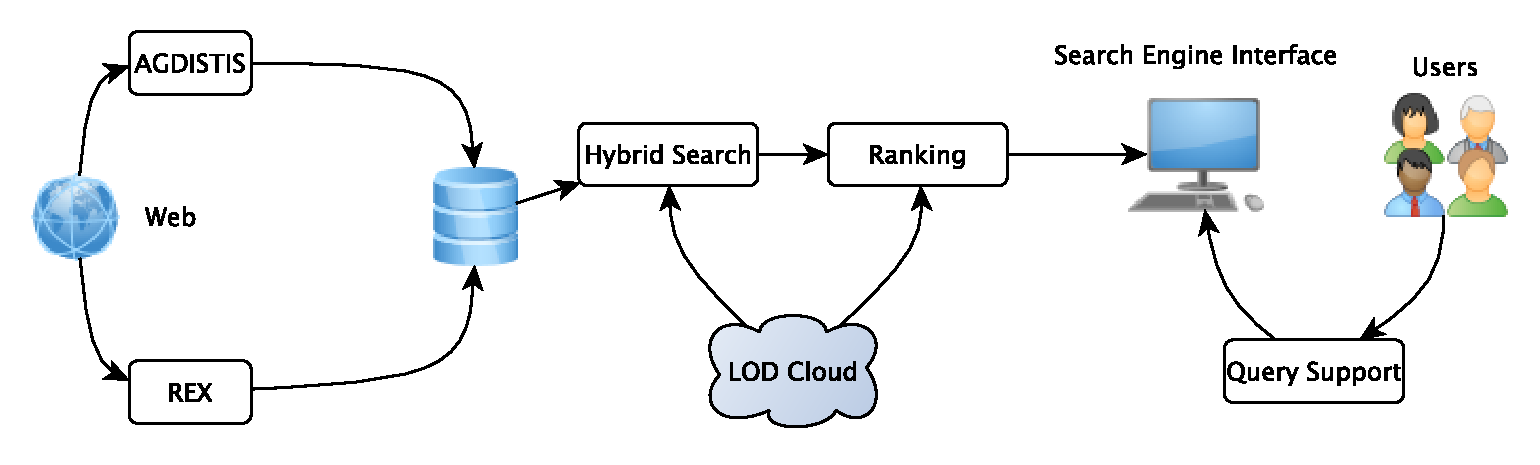
\includegraphics[width=\linewidth]{chapter_one/overview.pdf}
    \caption{Overview of the proposed information system architecture.}
    \label{overview}
\end{figure*}

The starting point of the proposed architecture is a two-fold data acquisition strategy based on a highly efficient, state-of-the-art industry Web crawler provided by our research partner \emph{Unister GmbH}.  

First, \emph{unstructured Web pages} from the crawled dataset, e.g., provided texts from news portals or agencies, are annotated by a standard NER algorithm~\cite{stanford} followed by a novel NED approach AGDISTIS~\cite{AGDISTIS}.
This NED approach has been developed to support arbitrary Linked Data knowledge bases to ensure future developments.
Moreover, AGDISTIS uses several NLP techniques to identify a set of candidate entities and identifies the correct with the help of the graph-based HITS algorithm. % and the resulting authority scores.
To prove the quality of AGDISTIS' results several corpora have been generated, evaluated and published. 
These corpora, called $N^3$~\cite{n3}, use the state-of-the-art serialization format \emph{NIF}~\cite{NIF} following the ``eating our own dogfood'' paradigm inherent to the Semantic Web community. 
$N^3$ are expected to form a novel gold standard in the areas of semantic named entity recognition and disambiguation.
Using $N^3$ and other well-known datasets, AGDISTIS has been proven to outperform the state-of-the-art algorithm AIDA~\cite{AIDA} by up to $16\%$ F-measure.
In the future, AGDISTIS will be evaluated against the framework of Cornolti et al.~\cite{cornolti} to provide a more comprehensive evaluation. 

Second, \emph{templated Web pages}, e.g., \url{http://www.imdb.com}, have been identified as another important source for answering user searches.
Therefore, REX~\cite{REX} has been developed during the early stage of this PhD work.
It is a web-scale semantic relation extraction framework capable to identify known as well as novel relations on Web pages creating RDF out of them.
REX combines a well-known wrapper induction technique~\cite{Crescenzi2013} for extracting XPath expressions, AGDISTIS as its NED algorithm and a consistency checker for the extracted relations based on ad-hoc generated schemas.
It has been shown that REX is able to generate new Linked Data triples with a precision of above $75\%$~\cite{REX}.

The resulting data from both pre-processing steps will serve as the underlying dataset for future research steps together with knowledge from the LOD Cloud.

Concerning the users' need for exploring the data space, %by enabling searches via keywords, natural language or even questions 
the next step is to \emph{support the formulation of queries}.
A huge potential within classical search engines is contained in inexact search queries, e.g., in terms of given a description only or a question.
Standard search engine methodologies fail at this point due to not being able to match keyword queries. 
In this thesis, we will support query formulation by providing on-the-fly recommended queries based on the real-time user input.
It is planned to use Linked Data such as \emph{BabelNet}\footnote{\url{http://babelnet.org/}} to find polysemes and synonyms within a query and thus enhancing the understanding of what the users actually mean.
Furthermore, three different standard approaches as well as a Linked Data-based grammar will be compared and evaluated against each other.
Another by-product of an according auto-completion approach is to teach the user which queries a search engine understands.

The research field of information retrieval/search and ranking has so far only been analysed theoretically within this doctoral work. 
In this thesis, a hybrid search engine is going to be implemented, i.e., an engine comprising a full-text information retrieval system enhanced by extracted Linked Data and a stake of LOD Cloud-based entity search.
Especially, the keyword-based search engine \emph{SINA}~\cite{sina} will be a starting point for further research. 

With respect to ranking algorithms, this PhD work focuses on two different research plans.
At first, a semantic extension of graph-based authority calculating algorithms will be investigated. 
Therefore, a master thesis has been looked after which analysed a context-driven enhancement of Stoyanovich's work~\cite{Stoyanovich}.
Initial results show an improvement compared to the baseline using the plain PageRank algorithm.
In parallel, an ensemble learning approach of Semantic Web-based ranking algorithms will be evaluated.

To summarize, the aforementioned steps will help building an integrated information system leveraging search engine performance using Linked Data.
Additionally--due to strong industry needs--this framework is going to be used in a real-life environment with web-scale amounts of users.
Finally, most of the source code will be published as open source and can be downloaded via the projects homepage\footnote{\url{http://aksw.org/RicardoUsbeck}}.

\section{Evaluation Plan and Conclusion}\label{conclusion}
This PhD work is dimensioned for three years. 
After intense literature reviews in the beginning of the first year the need for annotated Web data has been identified.
As a logical consequence, the development of AGDISTIS and REX had been finished by the end of the first year. 
Alongside, a gold standard ($N^3$) has been created to be able to evaluate the approaches mentioned above.

The second year will be used for developing and assessing the corresponding search and ranking procedures. 
To measure the quality of the \emph{auto-completion} technology, we assess different real-world query logs from our industry partner.
Thereby, we analyze how much characters are need to understand the query correct.
Additionally, we focus on the efficiency of the system in terms of milliseconds to react on a pressed key.

Considering the ranking evaluation, we will use standard precision, recall and f-measures as well as rank comparision measures, e.g., mean reciprocal rank. 
The underlying data is provided by the industry partner through human rater assessments and several comparisons to real-life search engines, e.g., Google or Wolfram Alpha.

Afterwards, the combined pipeline itself will be evaluated in a qualitative study using professionals and end users.
Therefore, empirical methods like Likert-scale questionnaires and direct relevance feedback will be used.


Next to refining already submitted work and optimizing the source code to meet industrial production standards, the developed approaches and algorithms will be refined in a spiral way if unpredictable results occur.
Thereby, upcoming ideas will be interweaved with the presented schedule creating a closed loop consisting of research question, development, evaluation and new research questions.

\chapter{Preliminaries}

%\begin{abstract}
Linked Data is becoming an increasingly popular method to publish data.
It is based on a simple set of rules and a number of widely adopted standards.
This introductory article aims at capturing the simplicity of Linked Data, and the concepts behind the related standards.
It will help the reader to understand the basic elements of Linked Data and its related technologies.
Using the example of a calendar app, we will highlight the practical advantages of using Linked Data for writing apps and publishing data in a completely decoupled way.
%\end{abstract}


\section{Introduction}
\label{intro}
Linked Data is a method to publish data on the Web, so that it can be connected to other datasets and create a Web of Data.
Four rules need to be followed in order to publish data as Linked Data~\cite{linkeddata-rules}:

\begin{enumerate}
\item Use URIs to name things
\item Use HTTP URIs so that they can be looked up
\item On lookup, provide useful information in standard formats
\item Provide links to other things
\end{enumerate}
%\todo[inline]{Was ist mit einer offenen Lizenz? Siehe 5 star data}

This chapter will describe the standards around Linked Data and their basic concepts.
Instead of focusing on completeness and technical correctness, we want to achieve an intuitive understanding in the interested but so far uninformed reader.
We refer to more comprehensive primers and the technical specifications in each section, so that the reader interested in more details can further deepen their knowledge.

Prerequisites for this chapter are merely a basic understanding of how the Web works.
It would be helpful if the reader was exposed to some basic ideas from data management, data structures, and knowledge representation.

Throughout the chapter we will use the example of writing a calendar application.
Our app will be able to deal with different time zones:
if the user enters a meeting like \textit{"Meeting at 9am in Atlanta"} the calendar tool should be able to translate the time to the local time zone, even if the meeting is being entered in Istanbul and shared with participants in Athens.

The chapter is structured as follows:
Section~\ref{semanticweb} explains the connection between Linked Data and the Semantic Web Vision.
Section~\ref{rdf} introduces the basic notions of RDF, especially the idea of an RDF graph and RDF triples.
Section~\ref{uri} describes URIs, the basic building blocks for such triples, and how they refer to the Web.
Section~\ref{http} then discusses how the Web is used for the distributed publishing of knowledge using the HTTP standard.
Secton~\ref{rdfs} extends the very simple expressivity of RDF, and discusses how languages like RDFS, OWL, and RIF are layered on top of it.
Section~\ref{sparql} introduces SPARQL, a query language for RDF graphs.
In Section~\ref{rdfa} we then go into more detail about the question how RDF is and can be serialized,
before we devote Section~\ref{xml} to the sometimes confusing relationship of RDF and XML.
We close in Section~\ref{conclusions} with a resum\'{e} on the state of Linked Data and an outlook on current developments.

\section{Vision of the Semantic Web}
\label{semanticweb}

Linked Data and \emph{Semantic Web} are sometimes used synonymously, although these two are rather different concepts.
The Semantic Web~\cite{semanticWeb} is a movement from the \texttt{Web of Documents} to the \texttt{Web of Data}.
The intention is to develop a Web that enables humans as well as machines to interact and work on existing data in way that creates an additional value.
To achieve this the data needs to be machine understandable, human manageable, linkable and storable in a standardized way.
Linked Data is the materialized implementation of the Semantic Web vision, executed by technologies like RDF, SPARQL, ontologies and many more decribed below.

\medskip

\textbf{Further readings}:
To get to know more about the Semantic Web vision we refer to the book~\cite{swbook} or the W3C Semantic Web website at \url{http://www.w3.org/standards/semanticweb/}.

\section{RDF: The basics}
\label{rdf}

RDF is a standardized model used for representing knowledge on the Web.
Knowledge representation in general enables to separate what a system does from what it knows~\cite{brachmannKR}, i.e., to make its knowledge explicit and not simply implicit in the program.
Decoupling knowledge from a program has several advantages, for example, it allows the knowledge base to be maintained externally, so that changes in the world may not even affect the code.

In the calendar app, one approach to deal with the different time zones would be to code the information into the program itself. 
We could simply have a function that, given a country or city name, returns the offset, implemented with a lot of \texttt{switch} or \texttt{if then else} statements.
A change in the timezone of a country would require rewriting the function and recompiling the whole application.
Instead, we could externalize the knowledge about countries and cites and their time zones.
The application would then load the knowledge base whenever it is needed, and behave accordingly.

There are many different ways to represent the knowledge in a way that the application can read it.
For example, we could have a database with tables of cities and countries and associated time zones.
We could have comma separated lists of cities for each time zone.
Or we could gather a consortium and define a standard for expressing time zone information, so that different developers can independently access this knowledge in their apps.%
\footnote{For time zones, this is roughly what happened, in form of the \textit{tz database}.}

RDF provides a generic, standardized model for representing knowledge.
Generic means, that it can be used in any domain, be it time zones, geographic data, genes, books, or anything else.
Standardized means that RDF has been specified in an explicit, reimplementable way, so that everyone can create software that can correctly read and write RDF documents.

The basic notions of RDF are triples and graphs.
Triples are used to express the given knowledge, piece by piece.
Each triple is built of three elements: a subject, a predicate, and an object.
In our example, a piece of knowledge could be expressed with the following triple:

\begin{verbatim}
 Turkey timezone EET .
\end{verbatim}

The subject in this triple is \texttt{Turkey}, the predicate is \texttt{timezone}, and the object \texttt{EET}.
The triple can intuitively be understood as having the same meaning as the English sentence \textit{"Turkey is in the timezone EET."}.

A graph consists of a set of triples.
It is called a graph, because the subjects and objects can be understood as nodes, connected with directed edges labeled with the given property.
The following example graph is visualized in Figure~\ref{fig:graph}.
\begin{verbatim}
 Turkey timezone EET .
 Greece timezone EET .
 Georgia timezone GET .
 EET borders GET .
 EET offset "2"^^int .
 GET offset "4"^^int . 
\end{verbatim}

\begin{figure}
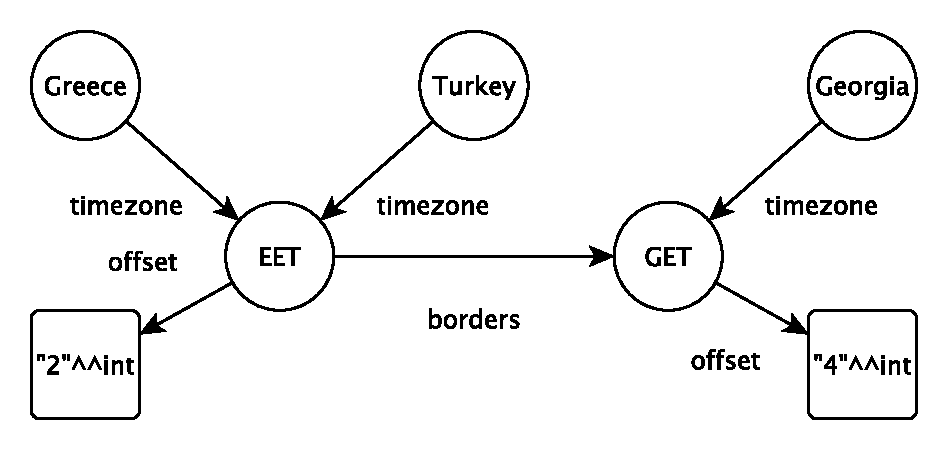
\includegraphics[width=\linewidth]{chapter_two/fig_graph.pdf}
\caption{Example of Linked Data used for the calender application}
\label{fig:graph}
\end{figure}

The last two triples in the example graph demonstrate the use of literal values in the object position: instead of a named node, that refers to an entity, we have a typed literal value.
The type in this case is \texttt{int}, which means that the values should be interpreted as integers.
The types available in RDF cover numbers, strings, booleans, dates, time durations, URIs, XML, and others.

\medskip

\textbf{Further readings}:
If you want to get deeper into the formalisms behind RDF have a look at the the RDF specification~\cite{rdf-spec}, 
the RDF primer~\cite{rdf-primer}, 
the specification for XSD datatype~\cite{xsd-part2}.
Relevant concepts we did not introduce are blank nodes, reification, named graphs and extensible datatypes~cf.~\cite{ namedgraphs,rdf-primer}.

\section{URIs: The words of the language}
\label{uri}

The big advantage of a graph-based model is that they can be easily be merged, by simply regarding a merger as a union of the triples in both graphs.
Many other models for knowledge representations, like tables or XML files, do not allow for such a generic merging.
But in order to provide a knowledge representation language that allows these kind of mergers, naming conflicts must be avoided.
In our example, \texttt{Georgia} refers to the caucasian country.
But now consider a second knowledge base about US states:

\begin{verbatim}
 Georgia timezone EST .
 SouthCarolina timezone EST .
 EST offset "-5"^^int .
\end{verbatim}

Since both Georgias -- the caucasian country and the US state -- are named the same, we would not be able to differentiate them.
Georgia now seems to be both in the timezone \texttt{GET} and \texttt{EST}!

To avoid this situation, all entities in Linked Data have to be referred to by unique names.
To achieve this, the names are given as URIs, most often HTTP URIs (just like websites).
The advantage of URIs is that anyone can register a prefix, and then create new names with this prefix.
The owner of the prefix is responsible for what the given name means.
So, the country Georgia could be named \texttt{http://example.org/countries\#Georgia} and the us state could be \texttt{http://example.org/usstates\#Georgia}.
As long as everyone defines new names in their own namespace only, naming conflicts can be avoided without constant coordination between all parties.

As URIs can be quite lengthy, often qualified names (or \textit{QNames}) are used.
They have the form \texttt{prefix:localName}.
Prefixes are defined locally to expand to a certain namespace, e.g., in our example we could define that the prefix \texttt{us} means the namespace \texttt{http://example.org/usstates\#}, and thus we could use the qualified name \texttt{us:Georgia} in order to refer to the complete URI \texttt{http://example.org/usstates\#Georgia}.

\medskip

\textbf{Further readings}:
To find more about the specification of URIs, see~\cite{uri} and for to get to know how to register a new URI scheme, have a look at~\cite{uri-registration}.
We did not speak about IRIs~\cite{iri} and other protocols besides HTTP, like FTP~\cite{ftp} or URN~\cite{urn}.

\section{HTTP: Distributed knowledge}
\label{http}

The second rule for publishing linked data is to use HTTP URIs.
The advantage is, that HTTP is a widely implemented protocol, that can be used over the Internet for accessing resources with a given HTTP URI.
For example, the above knowledge base could have itself the name \texttt{http://example.org/countries}.
Now a simple HTTP \texttt{GET} command like

\begin{verbatim}
 GET http://example.org/countries
\end{verbatim}

will return the knowledge base (it can be tried by entering the URI in a browser, but it is suggested for later as the result might be confusing at this point).

All entities are named with URIs, and the third rule of Linked Data asks to return information about the entity identified with a given URI when the URI is being dereferenced via HTTP.
This way, the Web can be used as vast knowledge space, where everyone can publish what they know about a given entity.

We can also use the URIs of others -- we do not have to publish URIs for all entities that we want to use ourselves.
For example, DBpedia is a widely used resource that publishes Linked Data based on Wikipedia's infoboxes~\cite{dbpedia}.
DBpedia offers URIs for all entities that have a Wikipedia page.
For example, Greece' Wikipedia page is \texttt{http://en.wikipedia.org/wiki/Greece} and, based on that, DBpedia defines the URI for Greece to be \texttt{http://dbpedia.org/resource/Greece}.
If this is entered into a browser, the browser redirects the user to a Web page about Greece in DBpedia.
If a Semantic Web application would have asked, DBpedia (prefix dbpedia) would have returned the RDF data instead.

So we could replace

\begin{verbatim}
 countries:Greece tz:timezone tz:EET .
\end{verbatim}

with using the DBpedia URI for Greece and get

\begin{verbatim}
 dbpedia:Greece tz:timezone tz:EET .
\end{verbatim}

This would have the advantage that now we can learn much more about Greece: the name of the country in different languages and alphabets, its population, the name of the head of state, etc.
Suddenly, our application can use knowledge from all over the Web.

Instead of simply replacing the URI, in our case we actually state that the URIs refer to the same entity, like this:

\begin{verbatim}
 countries:Greece owl:sameAs dbpedia:Greece .
\end{verbatim}

We see, that also properties can be reused from all over the Web.
In this case we use the term \texttt{sameAs} from the OWL vocabulary, which we will look at in the next section.

One advantage of using the Web as a knowledge base is that much knowledge is already published:
whereas our knowledge bases had information on some countries, Websites like Geonames or DBpedia offer lists of cities, and in which countries or US states they are located.
So regarding the cities we mentioned in the beginning of the article, the Web already offers the following pieces of knowledge:

\begin{verbatim}
 dbpedia:Istanbul dbo:country dbpedia:Turkey .
 dbpedia:Athens dbo:country dbpedia:Greece .
 dbpedia:Atlanta dbo:isPartOf dbpedia:Georgia_(U.S._state) .
\end{verbatim}

This allows us to just reuse the knowledge about cities from the Web of Data, for very little cost.

\medskip

\textbf{Further readings}:
For a deeper introduction of the HTTP protocol have a look at the HTTP specification~\cite{http}.

\section{RDFS, OWL and others: Adding expressivity}
\label{rdfs}

RDF allows us to express triples directly.
A very powerful method is to allow for implicit triples, by using more expressive semantics than simple triples.
We have seen one example already: \texttt{owl:sameAs} states that two URIs refer to the same entity.
That means that anything we say about \texttt{dbpedia:Greece} is also true about \texttt{countries:Greece}.
So now that we learnt that \texttt{dbpedia:Athens} is in \texttt{dbpedia:Greece}, we know that it is also in our own \texttt{countries:Greece}.

A number of languages build on top of RDF and extend it with more expressive semantics.
We will look at three of them, that are standardized by the W3C: RDFS, OWL, and RIF.

RDFS is the simplest one of them.
It allows us to describe class and property hierarchies:
for example, we have found on the Web cities connected to countries resp. US states.
The connection to the country was done using the \texttt{dbo:country}, to the state with \texttt{dbo:isPartOf}.
Now we can also define that everything that is connected via the former should also be connected through the latter.
In RDFS we do that with the following triple:

\begin{verbatim}
 dbo:country rdfs:subPropertyOf dbo:isPartOf .
\end{verbatim}

Now a reasoner who follows the RDFS semantics can infer that

\begin{verbatim}
 dbpedia:Istanbul dbo:isPartOf dbpedia:Turkey .
\end{verbatim}

is true, even though it was never stated explicitly.

OWL is much more expressive regarding the description of classes and properties:
for example, we can state that every city has to be in exactly one time zone, or that nothing can be both a U.S. state and a country, which could have helped to discover the error with the two Georgias automatically.

Since RDF allows only triples, such more complex statements need to be broken down to triples.
The statement \textit{"Every city is in exactly one time zone."} translates in RDF to the following four triples:

\begin{verbatim}
x:statement1 rdf:type owl:Restriction .
x:statement1 owl:onProperty tz:timezone .
x:statement1 owl:qualifiedCardinality "1"^^xsd:nonNegativeInteger .
x:statement1 owl:onClass dbo:City .
\end{verbatim}

Although this might seem a bit daunting, in reality these kind of triples are hidden either by more high-level syntaxes (see Section~\ref{rdfa}) or query tools (see Section~\ref{sparql}).

RIF is a different beast.
Whereas OWL is an expressive language to describe classes and properties, RIF is a way to express rules of them form \textit{if\ldots{}then\ldots{}}.
In our example, we might want to state that whenever a city is part of a country or state, and the country or state has a time zone, this is also the time zone of the city. Or, using the variables \texttt{?x}, \texttt{?y}, and \texttt{?z}:%
\footnote{We will not show how the rule is represented in RDF, as this looks even worse than the OWL statement above.}

If
\begin{verbatim}
 ?x dbo:isPartOf ?y .
 ?y tz:timezone ?z .
\end{verbatim}
then
\begin{verbatim}
 ?x tz:timezone ?z .
\end{verbatim}

RDFS, OWL, and RIF can, at least in theory, be all used together.
It depends on the used tools if a given semantics is understood: some reasoners support parts of OWL (so called fragments), some support only RDFS, other RIF, and a very few claim to support interesting combinations of all three languages, and sometimes beyond.

\medskip

\textbf{Further readings}:
The whole formalism can be found in the specifications for RDFS~\cite{rdfs}, OWL~\cite{owl}, and RIF~\cite{rif},but especially at the OWL primer in this book~\cite{dl-primer}.
We did not discuss questions of how to reason and about the complexity and decidability of reasoning. 
This is a big research topic, and in the last few years, it was advanced tremendously. 
We point to the DL Handbook as an entry point into this topic~\cite{dl-handbook}.
We also did not mention the different fragments of OWL, RIF, and the differences between OWL and OWL2, which can all be found in detail in the respective standards.
Besides the languages presented here, other languages like SKOS~\cite{skos} or WSML~\cite{wsml} exist, that can define other semantics.

\section{SPARQL: Querying RDF}
\label{sparql}

So far, we have described how to express knowledge: both simple facts (with RDF) and more expressive statements that enrich the knowledge base (in the previous section).
SPARQL provides a query language for RDF knowledge bases.

For example, assume that we have all the triples we have mentioned so far in one graph that we can query via SPARQL.
Let's also assume that the system providing the SPARQL endpoint understands the semantics of RDFS, OWL, and RIF.
Now we can ask for the offset for Athens:

\begin{verbatim}
 SELECT ?offset WHERE {
   dbpedia:Athens tz:timezone ?tz .
   ?tz tz:offset ?offset .
 }
\end{verbatim}

The system will return as a result the integer $2$.

Athens is in the country Greece. We know that from the Web.
Due to the OWL subproperty triple, we also know that to be in a country means to be part of it.
Because of the RIF rule, we can infer that if something is part of something, it also has the same timezone.
Based on this, the following two triples, the first one implicit, the second given explicitly, are in our knowledge base:

\begin{verbatim}
 dbpedia:Athens tz:timezone tz:EET .
 tz:EET tz:offset "2"^^xsd:int .
\end{verbatim}

A SPARQL query describes a triple pattern (similar to the one in the \textit{if}-part of RIF),
where symbols with a leading question mark are variables.
A SPARQL processor now tries to find values for the variables, so that the whole SPARQL pattern can be fulfilled by the knowledge base.
The SPARQL processors then returns a list of all possible answers for the selected variables,%
\footnote{That is, all variables following the introductory \texttt{SELECT} keyword, in this case \texttt{?offset}.}
i.e. in this case for all values that \texttt{?offset} can have so that the SPARQL query pattern matches in the knowledge base.
Given our query pattern, the two triples above are the only match in our knowledge base, and thus the result, \texttt{"2"\texttt{\char`\^}\texttt{\char`\^}xsd:int } will be returned as the only possible value for \texttt{?offset}.

SPARQL can be regarded as the main interface to access knowledge on the Web of Data.
Currently, the usual workflow to work with Linked Data is to find and gather trustworthy data from the Web, include some knowledge created for the task or tying together the data from the Web, put it all in one knowledge base, and then use SPARQL to get answers to the queries of interest to the given task.

\medskip

\textbf{Further readings}:
To find out more about SPARQL look at the specification for SPARQL~\cite{sparql}.
We did not discuss that SPARQL is not only a query language but also a protocol of how to acccess SPARQL endpoints.
We also did not discuss other types of queries: \texttt{DESCRIBE}, \texttt{ASK}, and \texttt{CONSTRUCT}, nor the powerful features of SPARQL to count, do math, regular expressions, named graphs, etc.

\section{RDFa and Co.: Serializations of RDF}
\label{rdfa}
What is a serialization?
To send around RDF graphs through the Web, we need somehow to write them down in documents, i.e. to serialize them in a sequence of tokens.
Throughout this chapter we have used a slightly simplified, triple-based serialization, N3~\cite{n3}.
N3 has the advantage, that the triple structure of the graph is very obvious.
Although, it is widely used, it has the disadvantage of not being standard.

There are a confusing number of serializations of RDF around, mostly due to the fact that the orginally standardized serialization in RDF/XML is considered to be not very pleasing.
Soon, further syntaxes were created, some of them also in XML (like TriX~\cite{trix}), some of them not (like N3 and its constrained version N-Triples~\cite{ntriples}.
Expressions in other languages like OWL and RIF were often very cumbersome to be translated to RDF (as shown in Section~\ref{rdfs}), and thus introduced serializations of their own, like the OWL Functional Syntax~\cite{owl2}, the OWL XML presentation syntax (a serialization of OWL directly in XML, instead of going through RDF~\cite{owl3}), the RIF syntaxes~\cite{rif}, etc.
Lately, JSON became a more prominent serialization format on the Web, and standards to represent the RDF data model in JSON are being worked on~\cite{json-ld}.

Besides serializations for pure RDF, there has been a second strand of embedding RDF in other file formats.
One of the main use cases for RDF is to provide flexible metadata about a file.
Embedding that metadata in the file itself has the advantage that the metadata is easier retained if the file gets moved, shared, changed, etc.
A growing number of file formats, like Adobe's (PDF, Photoshop, etc.) allow to embed RDF~\cite{xmp}.

The most relevant file format for the Web is obviously HTML itself, the language to describe Web pages and applications.
The RDFa standard offers how to markup and annotate elements of a Web page with RDF.
This allows a tool understanding RDFa to directly extract structured data out of a Website:
a page about an event can be pulled into a calendar,
a restaurant can be automatically filtered with the allergies of the user,
different shopping Websites can be thrown into one knowledge base and be compared directly, etc.

\medskip

\textbf{Further readings}:
If you want to find more serializations have a look at the specifications of RDFa~\cite{rdfa}, RDF in JSON~\cite{json-ld}, and RDF/XML~\cite{rdfxml}.
Also relevant is the ongoing conversation between the communities supporting Microformats~\cite{microformats}, Microdata~\cite{microdata}, and RDFa.

\section{XML: The confusing older brother}
\label{xml}

XML became the de-facto lingua france for data on the Web and beyond.
So it was natural, that it was assumed that RDF would be build on top of XML.
But in reality, the two are very different beasts:
XML describes a tree-based model, with a single root element, that has child elements in a strict order, and, who in turn, might have further child elements, in strict orders too, all strictly hierarchical.
RDF describes a graph-based model, where the order of the edges does not matter, and that is expressed as a simple set of triples.
XML schema defines a strict grammar for the elements in an XML documents, determining if an XML file is valid or not.
RDF schemas provide additional knowledge to infer implicit knowledge from a given RDF file, and can hardly be used to check the validity of an RDF file.
It is often easier to deal with valid XML files than with RDF files, because the developer has guarantees about the structure of the file.
On the other hand, RDF files are much easier to extend: one can simply add further triples, and, as long as they don't contradict the existing triples, the knowledge simply grows.
Two RDF files can always be simply merged automatically. For XML files in general, such an operation makes no sense.

With the benefit of hindsight, forcing RDF into an XML-based serialization was bound to lead to numerous problems without gaining the hoped-for advantages.
Many of the existing XML tools and workflows were actually unable to deal with RDF/XML files, so that the existing huge pool of experience and software could not be used to kickstart the Web of Data.

Today, XML does not play a prominent role for the Web of Data anymore.
Even if it gets further used as the main serialization format for RDF, its data model and the tools used with XML are loosing relevance.
It is an open question if this might change again, or if the rich set of software and experiences surrounding the XML world can be unlocked in favor of the Web of Data -- or the other way around.

\medskip

\textbf{Further readings}:
For more information about XML, see the XML specification~\cite{xml} or the XML Schema primer~\cite{xml-primer}.

\section{Conclusions and outlook}
\label{conclusions}

RDF is increasingly becoming the standard way to share data on the Web.
Using and publishing RDF is not an academic exercise anymore.
The flexibility and extensibility of RDF, together with the possibility to merge arbitrary RDF graphs, gives it a unique advantage compared to other wide spread data models.
Confusions surrounding its several serializations, especially the ill-received standard RDF/XML-serialization, a maybe too early focus on OWL, and the late availability of SPARQL, have probably hampered uptake.
Meanwhile, simple standards like Microformats and JSON have received considerable uptake.

The advantages and the genericity of Linked Data standards are being increasingly recognized.
Instead of introducing hundreds, if not thousands of APIs and heterogeneous formats, one common data model and query language can substantially decrease costs of data integration and data reuse.

End user interfaces to the Web of Data are still missing -- but maybe they always will.
Maybe the role of Linked Data is to be background technology:
no one asks for generic interfaces for end-users to SQL databases.
Maybe the Web of Data has a similar fate.

Still several practical issues remain unresolved:
\begin{itemize}
\item In general, SPARQL is too powerful and too expensive for the Web. It is far too easy to bring a SPARQL endpoint down with a few queries.
\item The multitude of serialization formats in practical use combined with the lack of standard formats besides RDF/XML hampers teaching about RDF and its uptake.
\item For a number of wide-spread use cases, no standards or even widely acknowledged best practices exist: how to express numbers with units, especially imperial units? How to express data that was valid at a given point in time? How to express time spans? How to deal with numerical precision? How to work with simple geographical and temporal reasoning, like inclusion?
\item The current standards allow fine-grained provenance information only through reification, a method, that is often strongly discouraged for several reasons.
\item The semantics break down under inconsistencies. There is currently no accepted way to deal with diversity in knowledge bases, even though this will play a crucial role on the Web. This ties in with questions of trust that have not yet been sufficiently tackled: given diverse data about an entity, maybe even contradictions, how to choose which sources to trust? How to make this trust transferable to the user?
\end{itemize}

The Web of Data, as part of the Web, is getting increasingly tangled with all aspects of our lives.
The growing number of intelligent apps and devices in our environment will have an ever-growing need to communicate with each other.
Imagining a future where our calendar app can support the flight finder app by restricting the departure and arrival times based on our agenda and the locations of our meetings and the airport, has become much easier today than it used to be only a few years ago.
Such a future is much easier to achieve when the applications and devices can all communicate in the same common and standard data model, and using the same interfaces.





\part{Knowledge Extraction from Unstructured Data}
\cleardoublepage
\ctparttext{
    The second part 
}
\newmdtheoremenv{ex}{Example}

\chapter{Knowledge-base Agnostic, Multilingual Entity Linking}
%\begin{abstract}
Over the last decades, several billion Web pages have been made available on the Web.
The ongoing transition from the current Web of unstructured data to the Web of Data yet requires scalable and accurate approaches for the extraction of structured data in RDF (Resource Description Framework) from these websites.
%Web/news data (WND) is the largest growing source of dynamic information on the Web outlining its importance in the upcoming Web of Data. 
One of the key steps towards extracting RDF from text is the disambiguation of named entities.
While several approaches aim to tackle this problem, they still achieve poor accuracy. % which is a permanently growing source of up-to-date information at the Web.
We address this drawback by presenting AGDISTIS, a novel knowledge-base-agnostic approach for named entity disambiguation.
Our approach combines the Hypertext-Induced Topic Search (HITS) algorithm with label expansion strategies and string similarity measures.
Based on this combination, AGDISTIS can efficiently detect the correct URIs for a given set of named entities within an input text. 
We evaluate our approach on eight different datasets against state-of-the-art named entity disambiguation frameworks.
%Moreover, we present an extension based on topic modeling which improves the quality of the extraction in difficult cases by up to $3\%$.
Our results indicate that we outperform the state-of-the-art approach by up to $29\%$ F-measure.
%\end{abstract}

\section{Introduction}
The vision behind the Web of Data is to provide a new machine-readable layer to the Web where the content of Web pages is annotated with structured data (e.g., RDFa~\cite{rdfa}).
However, the Web in its current form is made up of at least 15 billion Web pages.\footnote{Data gathered from \url{http://www.worldwidewebsize.com/} on January 4th, 2014.}
Most of these websites are unstructured in nature.
Realizing the vision of a usable and up-to-date Web of Data thus requires scalable and accurate natural-language-processing approaches that allow extracting RDF from such unstructured data.
Three tasks play a central role when extracting RDF from unstructured data: named entity recognition (NER), named entity disambiguation (NED), also known as entity linking~\cite{Mihalcea:2007:WLD:1321440.1321475}, and relation extraction (RE).
For the first sentence of Example~\ref{ex:obama}, an accurate named entity recognition approach would return the strings \texttt{Barack Obama} and \texttt{Washington, D.C.}.
A high-quality DBpedia-based named entity disambiguation (NED) approach would use these already recognized named entities and map the strings \texttt{Barack Obama} resp. \texttt{Washington, D.C.} to the resources \texttt{dbr:Barack\_Obama} and \texttt{dbr:Washington,\_D.C.}\footnote{\texttt{dbr:} stands for \url{http://dbpedia.org/resource/}}~\cite{dbpedia-swj}.
\begin{ex}
Barack Obama arrived this afternoon in Washington, D.C.. President Obama's wife Michelle accompanied him.
\label{ex:obama}
\end{ex}
While NER has been explored extensively over the last decades~\cite{StanfordNER}, the disambiguation of named entities,\,i.e., the assignment of a resource's URI from an existing knowledge base to a string that was detected to label an entity remains a difficult task.

Current NED approaches suffer from two major drawbacks:
First, they poorly perform on Web documents~\cite{RatinovRo09}.
This is due to Web documents containing resources from different domains within a narrow context.
An accurate processing of Web data has yet been shown to be paramount for the implementation of the Web of Data~\cite{GER+13}.
%, Web data is a very worthwhile source of latest information which is often not yet captured in any knowledge base. 
Well-know approaches such as \emph{Spotlight}~\cite{spotlight} and \emph{TagMe 2}~\cite{TagMe2} have been designed to work on a particular knowledge base.
However, Web data contains resources from many different domains.
%Ttha named entity disambiguation framework has to be able to work on any knowledge base in order to capture content from different domains.
Hence, we argue that NED approaches have to be designed in such a way that they are agnostic of the underlying knowledge base.
%Being capable of using specialized or language-specific knowledge bases should lead to high F-measures. 
Second, most state-of-the-art approaches rely on exhaustive data mining methods~\cite{Cucerzan07,rat:rot} or algorithms with non-polynomial time complexity~\cite{Kleb11WIMS}.
However, given the large number of entities that must be disambiguated when processing Web documents, scalable NED approaches are of central importance to realize the Semantic Web vision.
%\todo[inline]{Micha: The sentence "Hence, we argue that NED..." is not really good. From my point of View it sounds like "A NED-algorithm has to use more than one KB at the same time".}

In this paper, we address these drawbacks by presenting AGDISTIS, a novel NED approach and framework.
AGDISTIS achieves \emph{higher F-measures} than the state of the art while remaining \emph{polynomial in its time complexity}.
AGDISTIS achieves these results by combining the HITS algorithm~\cite{HITS} with label expansion and string similarity measures.
Overall, our contributions can be summed up as follows:
(1) We present AGDISTIS, an accurate and scalable framework for disambiguating named entities that is agnostic to the underlying knowledge base (KB) and show that we are able to outperform the state of the art by up to $29\%$ F-measure on these datasets.
%\todo[inline]{description of datasets? multilingual, multi-domain}
(2) We show that our approach has a quadratic time complexity. Thus, it scales well enough to be used even on large knowledge bases.
(3) We evaluate AGDISTIS on eight \emph{well-known and diverse open-source datasets}.\footnote{Further data, detailed experimental results and source code for this paper are publicly available on our project homepage \url{http://aksw.org/Projects/AGDISTIS}.} 

The rest of this paper is organized as follows: We first give a brief overview of related work in Section~\ref{sec:relatedwork}. 
Then, we introduce the AGDISTIS approach in Section~\ref{sec:approach}. %comprising an overview, the way AGDISTIS detects candidates and the disambiguation algorithm itself. 
%We formalize the task of NED in Section~\ref{sec:ned}.
After presenting the datasets, we evaluate our approach against the state of the art frameworks AIDA and TagMe 2 and the well-known DBpedia Spotlight. 
Furthermore, we measure the influence of using surface forms,\,i.e., synonymous label for a specific resource, in Section~\ref{sec:eval}. 
%\todo{surface form richtig erklärt?}
%We analyze the contribution of certain properties to our disambiguation approach in the same section. 
We conclude in Section~\ref{sec:conclusion} by highlighting research questions that emerged from this work.
%Our approach is open-source and can be found at \url{http://aksw.org/Projects/AGDISTIS}.
A demo of our approach (integrated into the Named Entity Recognition framework FOX~\cite{FOX}) can be found at \url{http://fox.aksw.org}. 


\section{Related Work}
\label{sec:relatedwork}
AGDISTIS is related to the research area of Information Extraction~\cite{nad:sek} in general and to NED in particular.
Several approaches have been developed to tackle NED. 
Cucerzan presents an approach based on extracted Wikipedia data towards disambiguation of named entities~\cite{Cucerzan07}.
The author aims to maximize the agreement between contextual information of Wikipedia pages and the input text by using a local approach.
%\todo{What's a local approach?}
\emph{Epiphany}~\cite{epiphany} identifies, disambiguates and annotates entities in a given HTML page with RDFa. 
Ratinov et al.~\cite{rat:rot} described an approach for disambiguating entities from Wikipedia KB. 
The authors argue that using Wikipedia or other ontologies can lead to better global approaches than using traditional local algorithms which disambiguate each mention separately using,\,e.g., text similarity. %for word sense disambiguation.
Kleb et al.~\cite{Kleb11WIMS,KlebESWC10} developed and improved an approach using ontologies to mainly identify geographical entities but also people and organizations in an extended version. 
These approaches use Wikipedia and other Linked Data KBs.
LINDEN~\cite{LINDEN} is an entity linking framework that aims at linking identified named entities to a knowledge base.
To achieve this goal, LINDEN collects a dictionary of the surface forms of entities from different Wikipedia sources, storing their count information.

Wikipedia Miner~\cite{milne2008learning} is the oldest approach in the field of \emph{wikification}.
Based on different machine learning algorithms, the systems disambiguates w.r.t. prior probabilities, relatedness of concepts in a certain window and context quality. 
The authors evaluated their approach based on a Wikipedia as well as an AQUAINT subset. 
Unfortunately, the authors do not use the opportunities provided by Linked Data like DBpedia.

Using this data the approach constructs candidate lists and assigns link probabilities and global coherence for each resource candidate.
The AIDA approach~\cite{AIDA} for NED tasks is based on the YAGO2\footnote{\url{http://www.mpi-inf.mpg.de/yago-naga/yago/}} knowledge base and relies on sophisticated graph algorithms. 
Specifically, this approach uses dense sub-graphs to identify coherent mentions using a greedy algorithm enabling Web scalability. 
Additionally, AIDA disambiguates w.r.t.~similarity of contexts, prominence of entities and context windows.

Another approach is DBpedia Spotlight~\cite{spotlight}, a framework for annotating and disambiguating Linked Data Resources in arbitrary texts.
In contrast to other tools, Spotlight is able to disambiguate against all classes of the DBpedia ontology.
Furthermore, it is well-known in the Linked Data community and used in various projects showing its wide-spread adoption.\footnote{\url{https://github.com/dbpedia-spotlight/dbpedia-spotlight/wiki/Known-uses}}
Based on a vector-space model and cosine similarity DBpedia Spotlight is publicly available via a web service\footnote{\url{https://github.com/dbpedia-spotlight/dbpedia-spotlight/wiki/Web-service}}.

In 2012, Ferragina et al. published a revised version of their disambiguation system called TagMe 2.
The authors claim that it is tuned towards smaller texts,\,i.e., comprising around 30 terms.
TagMe 2 is based on an anchor catolog (\texttt{<a>} tags on Wikipedia pages with a certain frequency), a page catalogue (comprising all original Wikipedia pages,\,i.e., no disambiguations, lists or redirects) and an in-link graph (all links to a certain page within Wikipedia).
First, TagMe 2 identifies named entities by matching terms with the anchor catalog and second disambiguates the match using the in-link graph and the page catalog via a collective agreement of identified anchors. 
Last, the approach discards identified named entities considered as non-coherent to the rest of the named entities in the input text.  

In 2014, Babelfy~\cite{babelfy} has been presented to the community.
Based on random walks and densest subgraph algorithms Babelfy tackles NED and is evaluated with six datasets, one of them the later here used AIDA dataset. 
In constrast to AGDISTIS, Babelfy differentiates between word sense disambiguation, i.e., resolution of polysemous lexicographic entities like \emph{play}, and entity linking, i.e., matching strings or substrings to knowledge base resources.
Due to its recent publication Babelfy is not evaluated in this paper.

Recently, Cornolti et al.~\cite{cornolti} presented a benchmark for NED approaches.
The authors compared six existing approaches, also using DBpedia Spotlight, AIDA and TagMe 2, against five well-known datasets. % on different tasks and with different measures.
Furthermore, the authors defined different classes of named entity annotation task, e.g. \emph{`D2W'}, that is the disambiguation to Wikipedia task which is the formal task AGDISITS tries to solve.
We consider TagMe 2 as state of the art w.r.t. this benchmark although only one dataset has been considered for this specific task.
We analyze the performance of DBpedia Spotlight, AIDA, TagMe 2 and our approach AGDISTIS on four of the corpora from this benchmark in Section~\ref{sec:eval}.

\section{The AGDISTIS Approach} 
\label{sec:approach}

\subsection{Named Entity Disambiguation}
\label{sec:ned}

The goal of AGDISTIS is to detect correct resources from a KB $K$ for a vector $N$ of $n$ a-priori determined named entities $N_1,\ldots,N_n$ extracted from a certain input text $T$.
In general, several resources from a given knowledge base $K$ can be considered as candidate resources for a given entity $N_i$.
For the sake of simplicity and without loss of generality, we will assume that each of the entities can be mapped to $m$ distinct candidate resources.
Let $C$ be the matrix which contains all candidate-entity mappings for a given set of entities.
The entry $C_{ij}$ stands for the $j^{th}$ candidate resource for the $i^{th}$ named entity. 
Let $\mu$ be a family of functions which maps each entity $N_i$ to exactly one candidate $C_{ij}$. 
We call such functions \emph{assignments}.
The output of an assignment is a vector of resources of length $|N|$ that is such that the $i^{th}$ entry of the vector maps with $N_i$.

Let $\psi$ be a function which computes the similarity between an assignment $\mu(C,N)$ and the vector of named entities $N$.
The \emph{coherence} function $\phi$ calculates the similarity of the knowledge base $K$ and an assignment $\mu$, cf. Ratinov et al.~\cite{rat:rot}, to ensure the topical consistency of $\mu$.
The coherence function $\phi$ is implemented by the HITS algorithm, which calculates the most pertinent entities while the similarity function $\psi$ is,\,e.g., string similarity.
Given this formal model, the goal is to find the assignment $\mu^\star$ with
\begin{equation*}
\mu^\star= \operatorname*{arg\,max}\limits_{\mu}\left(\psi(\mu(C,N), N) + \phi(\mu(C,N),K)\right).
\end{equation*}

The formulation of the problem given above has been proven to be NP-hard, cf. Cucerzan et al.~\cite{Cucerzan07}.
Thus, for the sake of scalability, AGDISTIS computes an approximation $\mu^{+}$ by using HITS, a fast graph algorithm which runs with an upper bound of $\Theta(k\cdot |V|^2)$ with $k$ the number of iterations and $|V|$ the number of nodes in the graph.
Furthermore, using HITS leverages 1) scalability, 2) well-researched behaviour and 3) the ability to explicate semantic authority. 

\subsection{Architecture}
\begin{figure*}[h!tb]
\centering
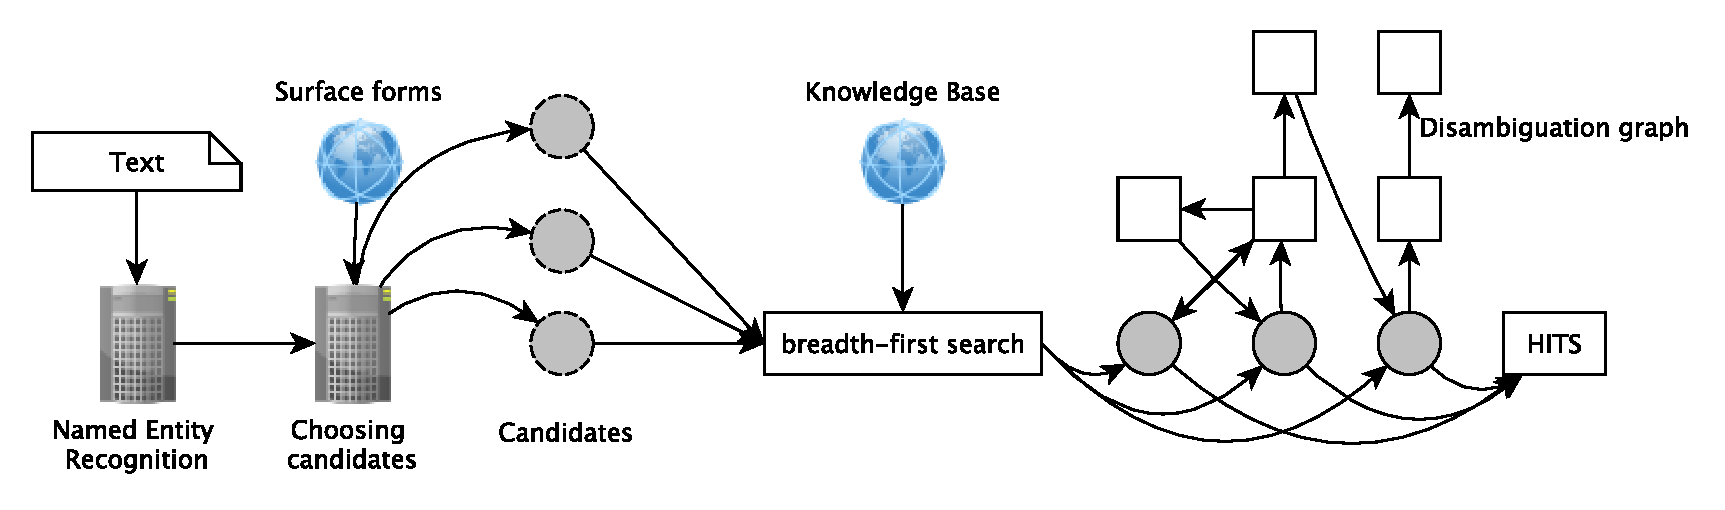
\includegraphics[width=\linewidth]{chapter_three/unstructured_annotation/fig/overview.pdf}
\caption{Overview of AGDISTIS.}
\label{fig:overview_agdistis}
\end{figure*}
%\todo[inline]{caption bei Änderung des Titels anpassen}

Our approach to NED thus consists of three main phases as depicted in Figure~\ref{fig:overview_agdistis}.
Given an input text $T$ and a named entity recognition function (e.g., FOX~\cite{FOX}), we begin by retrieving all named entities from the input text.
Thereafter, we aim to detect candidates for each of the detected named entities.
To this end, we apply several heuristics and make use of known surface forms~\cite{spotlight} for resources from the underlying KB.
The set of candidates generated by the first step is used to generate a disambiguation graph. 
Here, we rely on a graph search algorithm which retrieves context information from the underlying KB. 
Finally, we employ the HITS algorithm to the context graph to find authoritative candidates for the discovered named entities.
We assume that the resources with the highest authority values represent the correct candidates.
All algorithms in AGDISTIS have a polynomial time complexity, leading to AGDISTIS also being polynomial in time complexity.
Choosing candidates relates to the notion of $\phi$ while calculating the authority values confers to $\psi$.
In the following, we present each of the steps of AGDISTIS in more detail.

\subsection{Candidate Detection}\label{choosing}

In order to find the correct disambiguation for a certain set of named entities, we first need to detect candidate resources in the KB. 
We begin by creating an index comprising all labels of each resource.
Our approach can be configured to use any set of properties as labeling properties (e.g., those in Ell et al.~\cite{ELL+11}). 
For our experiments, we only considered \texttt{rdfs:label} as labeling property.
In addition, our approach can make use of known \emph{surface forms} for each of the resources in case such knowledge is available~\cite{spotlight}.
These are simply strings that are used on the Web to refer to given resources.
Surface forms are simply added to the set of available labels for each resource, cf.\ Section~\ref{eval}.
In this paper, we do not consider abbreviations although these could be easily regarded by adding further labels into the KB (e.g., via WordNet\footnote{\url{http://wordnet.princeton.edu/}}).
%\todo[inline]{remove the above sentence because of missing scientific eval?}

Next to searching the index we apply a \emph{string normalization} approach and an \emph{expansion policy} to the input text:
The string normalization is based on eliminating plural and genitive forms, removing common affixes such as postfixes for enterprise labels and ignoring candidates with time information (years, dates, etc.) within their label.
For example, the genitive \texttt{New York's} is transformed into \texttt{New York}, the postfix of \texttt{Microsoft Ltd.} is reduced to \texttt{Microsoft} and the time information of \texttt{London 2013} is ignored.
Our \emph{expansion policy} is a time-efficient approach to coreference resolution, which plays a central role when dealing with text from the Web, cf.~Singh et al.~~\cite{singh}. 
In web and news documents, named entities are commonly mentioned in their full length the first time they appear, while the subsequent mentions only consist of a substring of the original mention due to the brevity of most news data.
For example, a text mentioning Barack Obama's arrival in Washington D.C. will commonly contain \texttt{Barack Obama} in the first mention of the entity and use strings such as \texttt{Obama} or \texttt{Barack} later in the same text (see Example~\ref{ex:obama}).
We implement this insight by mapping each named entity label (e.g., \texttt{Obama}) which is a substring of another named entity label that was recognized previously (e.g., \texttt{Barack Obama}) to the same resource ,\,i.e., \texttt{dbr:Barack\_Obama}.
If there are several possible expansions, we choose the shortest as a fast coreference resolution heuristic for web documents.
Without the expansion policy AGDISTIS suffers from a loss of accuracy of $\approx4\%$.

%This is simply due to humans readers being able to carry out a co-reference analysis on the fly.

%Internally, AGDISTIS begins its disambiguation by employing the string expansion policy\footnoterecall{myfootnote}.
%Our policy stores all named entity strings in order of their string length.
%If we recognize an entity string matching a part of an already processed entity, we expand the current string to the one stored earlier.
%This assumes both named entities mention the same instance.


%After expanding named entities we harness additional well-known linguistic heuristics.
%Named entities occur often in plural and genitive forms,\,i.e., AGDISTIS tries to identify and stem those words. 
%For example, the genitive form of the named entity \texttt{Obama's} is transformed into \texttt{Obama}.
%Additionally, AGDISTIS reduces plural strings such as \texttt{Obamas} to the singular form \texttt{Obama}.
%Another heuristic is to remove common affixes. 
%For example, we remove affixes which stands for the form of enterprises, such as \emph{corp} and \emph{ltd},\,e.g., \texttt{Hanover Insurance Corp.} is shrunk to \texttt{Hanover Insurance} in order to find candidates for this string in the KB.  	
%We observed a significant data quality problem considering affixes in the examined knowledge bases.
%AGDISTIS also eliminates candidates with years and dates within the label so as to be time-independent and to prune the search space.
%One key advantage of Linked Data is the possibility to retrieve a class for each instance in a KB.
%By using entity types (obtained via the \texttt{rdf:type} property), a domain fitting of possible candidates is implemented, narrowing the search space. 
Additionally, AGDISTIS can be configured to fit named entities to certain domains to narrow the search space.
Since our goal is to disambiguate persons, organizations and places, AGDISTIS only allows candidates of the types mentioned in Table~\ref{tab:tableOfClasses} when run on DBpedia and YAGO2.
Adding general types will increase the number of candidates and thus decrease the performance.
Obviously, these classes can be altered by the user as required to fit his purposes. 

\begin{table*}[htb!]
\centering
 \caption{DBpedia  and YAGO2 classes used for disambiguation classes. Prefix \texttt{dbo} stands for \texttt{http://dbpedia.org/ontology/}, \texttt{foaf} for \texttt{http://xmlns.com/foaf/0.1/} and \texttt{yago} for \texttt{http://yago-knowledge.org/resource/}.}
 \begin{tabular}{lll}
	\toprule
\textbf{} & \textbf{Class} & \texttt{\textbf{rdf:type}}\\
\midrule
DBpedia & Person & dbo:Person, foaf:Person\\
DBpedia & Organization & dbo:Organization, dbo:WrittenWork (e.g., Journals) \\
DBpedia & Place & dbo:Place, yago:YagoGeoEntity \\
\midrule
YAGO2 & Person & yago:yagoLegalActor  \\
YAGO2 & Organization & yago:yagoLegalActor, \\
  &   &  yago:wordnet\_exchange\_111409538 (e.g., NASDAQ) \\
YAGO2 & Place & yago:YagoGeoEntity \\
\bottomrule
\label{tab:tableOfClasses}
 \end{tabular}
 \end{table*}

\begin{algorithm}[htb!]
\KwData{label of a certain named entity $N_i$, $\sigma$ trigram similarity threshold}
\KwResult{$C$ candidates found}
$C \longleftarrow \emptyset$\;
{\bf label } $\longleftarrow$ {\bf normalize(label)}\;
{\bf label } $\longleftarrow$ {\bf expand(label)}\;
$ \displaystyle \bar C \longleftarrow$ {\bf searchIndex(label)}\;
\For{{\bf c} $\in \bar C$}{
    \If{$\neg${\bf c .matches([0-9]$^+$)}}{
        %\If{$\neg${\bf isDisambiguationSite(c})} {
         %          {\bf continue}\;
          %      }
        \If{{\bf trigramSimilarity(c, label)}$ \geq \sigma$}{
            \If{{\bf fitDomain(c)}} {
                $C \longleftarrow C \cup $ {\bf c}\;
            }
        }
        % The same as the two ifs above but with a continue
        %\If{{\bf trigramSimilarity(c, label)}$ < \sigma$} {
        %           {\bf continue}\;
        %        }
        %% {\bf c} $\longleftarrow$ {\bf redirect(c)}\;
        %\If{{\bf fitDomain(c)}} {
        %     $C \longleftarrow C \cup $ {\bf c}\;
        %        } 
        %}
    }
}
\caption{Searching candidates for a label.}
\label{findingCandidates}
\end{algorithm}

The resulting candidate detection approach is explicated in Algorithm~\ref{findingCandidates}.
%If a KB provides redirect and disambiguation URLs, AGDISTIS can benefit from them.
%\todo[inline]{added  a virtual function in this algorithm 1 for the grammatical functions}
%For example, it is straightforward to use \texttt{dbo:wikiPageRedirects} for identifying multiple labels for one instance. 
%Of course AGDISTIS ignores disambiguation entities as they would not help accomplishing the disambiguation goal and finding $\mu^{+}$. 
%\todo[inline]{AN:What's a disambiguation entity?}
In its final step, our system compares the heuristically obtained label with the label extracted from the KB by using \emph{trigram similarity} which is an n-gram similarity with $n=3$. 


\subsection{Computation of Optimal Assignment}

Given a set of candidate nodes, we begin the computation of the optimal assignment by constructing a disambiguation graph $G_d$ with search depth $d$.
To this end, we regard the input knowledge base as a directed graph $G_K = (V, E)$ where the vertices $V$ are resources of $K$, the edges $E$ are properties of $K$ and $x,y\in V, (x,y) \in E \Leftrightarrow \exists p : (x, p, y) \mbox{ is an RDF triple in }K$.
Given the set of candidates $C$, we begin by building an initial graph $G_0 = (V_0, E_0)$ where $V_0$ is the set of all resources in $C$ and $E_0=\emptyset$. %$\forall (x, y) \in V_0^2, (x, y) \in E_0 \Rightarrow (x, y) \in K$.
Starting with $G_0$ we extend the graph in a breadth-first search manner.
Therefore, we define the extension of a graph $G_i = (V_i, E_i)$ to a graph $\rho(G_i) = G_{i+1} = (V_{i+1}, E_{i+1})$ with $i=0, \ldots, d$ as follows:
\begin{equation}
V_{i+1} = V_i \cup \{y : \exists x \in V_i \wedge (x, y) \in E\}
\end{equation}
\begin{equation}
E_{i+1} = \{(x,y) \in E: x, y \in V_{i+1}\}
\end{equation}
We iterate the $\rho$ operator $d$ times on the input graph $G_0$ to compute the initial disambiguation graph $G_d$.

%Empirically, we see no effect on the \mbox{F-measure} when using spread activation instead~\cite{Kleb11WIMS} (despite the obvious extra computational costs).

After constructing the disambiguation graph $G_d$ we need to identify the correct candidate node for a given named entity.
Using the graph-based HITS algorithm we calculate authoritative values $x_a,y_a$ and hub values $x_h,y_h$ for all $x,y\in V_d$.
We initialize the authoritative and hub values (3) and afterwards iterate the equations (4) $k$ times as follows: 
\begin{align*}
\forall x \in V_d, x_a=x_h=\frac{1}{|V_d|} &\text{ (3) and } 
x_a\longleftarrow  \sum_{(y,x)\in E_d} y_h, \quad
y_h\longleftarrow \sum_{(y,x)\in E_d} x_a \text{(4)}
\end{align*}
We choose $k$ according to Kleinberg~\cite{HITS},\,i.e., 20 iterations, which suffice to achieve convergence in general. %d authoritative values $x_a$ and hub values $y_h$.
Afterwards we identify the most authoritative candidate $C_{ij}$ among the set of candidates $C_i$ as correct disambiguation for a given named entity $N_i$. %sort the nodes according to their authoritative values in descending order. 
%The first candidate for a certain named entity is assumed to be the correct disambiguation.
When using DBpedia as KB and $C_{ij}$ is a redirect AGDISTIS uses the target resource. %follows redirecting resources transitively. %can use redirections to di%maps redirecting resources to their most authoritative redirection.
AGDISTIS' whole procedure is presented in Algorithm~\ref{algooverview}.
As can be seen, we calculate $\mu^{+}$ solely by using polynomial time complex algorithms.
%Thus, we observe on average better run time performance than the state-of-the-art approach AIDA, see Section~\ref{results}. % Appendix Figure 3).
%\todo[inline]{Again, we have no Appendix here}
\begin{algorithm}
\KwData{$N=\{N_1,N_2\dots N_n\}$ named entities, $\sigma$ trigram similarity threshold, $d$ depth, $k$ number of iterations}
\KwResult{$C = \{C_1,C_2\dots C_n\}$ identified candidates for named entities}
$E \longleftarrow \emptyset$\;
$V \longleftarrow${\bf insertCandidates($N, \sigma$)}\;
$G \longleftarrow (V,E)$\;
$G \longleftarrow${\bf breadthFirstSearch($G,d$)}\;
{\bf HITS($G(V,E), k$)}\;
{\bf sortAccordingToAuthorityValue(V)}\;
\For{$N_i \in N$} {
    \For{$v \in V$}{
        \If{$v$ {\bf is a candidate for} $N_i$  }{
              {\bf store($N_i$,$v$)}\;
              {\bf break}\;
          }
     }
}
\caption{Disambiguation Algorithm based on HITS and Linked Data.}\label{algooverview}
\end{algorithm}

For our example, the graph depicted in Figure~\ref{fig:example} shows an excerpt of the input graph for the HITS disambiguation algorithm when relying on DBpedia as knowledge base. 
%Depending on the used KB properties may exist that lead to bi-directional edges (e.g., \texttt{sex} vs. \texttt{fatherOf}).
The results can be seen in Table~\ref{tab:example}. 
%Obviously a disambiguation towards the correct named entity URIs is possible.
%\todo{what happens if the KB does not contain the correct entity, does the algorithm answer null, but is encompanied with closed world assumption, we know all entities we annotated}
%Since we assume a closed-world scenario our algorithm supposes every entity to be in the KB.

\begin{figure}[htbp]
	\begin{minipage}[b]{0.57\textwidth} 
       % \begin{figure}
         \centering
        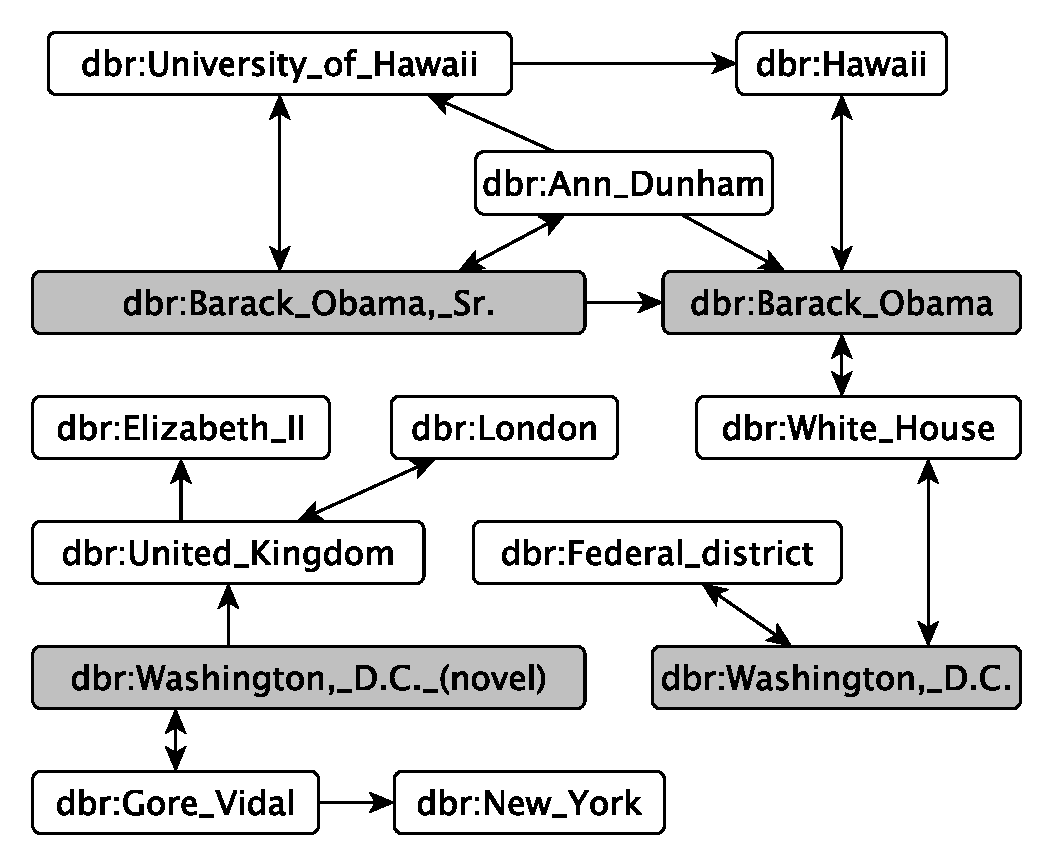
\includegraphics[width=\linewidth]{chapter_three/unstructured_annotation/fig/exampleGraph.pdf}
        \caption{One possible graph for the example sentence, with candidate nodes in grey.}
        \label{fig:example}
      %  \end{figure}
    \end{minipage}
	\hfill
	\begin{minipage}[b]{0.42\textwidth}
       % \begin{table}
        \centering
        \begin{tabular}{lc}
            \toprule
            \textbf{Node}  & \textbf{$x_a$} \\
            \midrule
            db:Barack\_Obama & 0.273 \\
            db:Barack\_Obama,\_Sr. & 0.089 \\
            db:Washington,\_D.C. & 0.093 \\
            db:Washington,\_D.C.\_(novel) & 0.000 \\
            \bottomrule
        \end{tabular}
        \captionof{table}{Authority weights for example graph.}
        \label{tab:example}
        \vspace{1.8cm}
       % \end{table}
	\end{minipage}
\end{figure}

%%Idea of the extension
%The most words of a document given to AGDISTIS are no named entities.
%Therefore, AGDISTIS does not use them in its workflow.
%Because a human reader would use all words for the disambiguation task we thought of an extension of AGDISTIS which uses the additional words, too.
%With these words AGDISTIS would be able to recognize the topical structure of the document and could use these information for the disambiguation task.
%Therefore, we added an extension which uses topic modeling to consider the topical structure.

%%what is topic modeling
%\emph{Probabilistic topic modeling} is a research area that aims to discover thematic information inside large corpora \cite{Blei:2012:PTM:2133806.2133826}.
%It is based on the definition of generative models that describe the creation of documents and how this process is influenced by latent topics.
%A very famous model is \emph{Latent Dirichlet Allocation (LDA)} \cite{Blei:2003:LDA:944919.944937}.
%Its generative process is based on a set of Topics $T$ and a vocabulary $V$.
%For the creation of a document $d$ the distribution of the topics inside this document $\theta_d=\left \{P(t_0|d), \ldots, P(t_{|T|}|d) \right \}$ is sampled.
%After that for every $i$th-word the id $z_i$ of a topic $t_{z_i}$ is sampled from $\theta_d$.
%Every topic $t \in T$ has a vector $\phi_{t}=\left \{P(w_0|t), \ldots, P(w_{|V|}|t) \right \}$ which defines the probabilities of all words under this topic.
%After $z_i$ has been sampled the word is sampled from $\phi_{t_{z_i}}$ \cite{Blei:2012:PTM:2133806.2133826}.
%Figure TODO shows the graphical model of LDA.
%The figure contains $\alpha$ and $\beta$ which are hyperparameter for the $\theta$ and $\phi$ distributions respectively.
%\todo[inline]{Add graphic with plate notation}

%In figure TODO all variables are white except the word $w$ which is shaded.
%This means that $w$ is the only variable which can be observed and all other variables are latent.
%So starting with the observable words inside of the documents of a corpus the other variables have to be inferenced.
%Because a direct solution of the inference problem is intractable there are several algorithms for approximating the variables \cite{Blei:2012:PTM:2133806.2133826}.
%For our experiments we used Mallet which contains an implementation of Gibbs-Sampling \cite{McCallumMALLET,griffiths2004finding}.

%\todo[inline]{* definition \newline* LDA \newline* generative model \newline* how do we use it \newline* where does the model come from\newline * \textbf{what are we doing with the model and the texts}}

\section{Evaluation}
\label{sec:eval}

\subsection{Experimental Setup}
\label{eval}
The aim of our evaluation was two-fold.
First, we wanted  to determine the F-measure achieved by our approach on different datasets.
Several definitions of F-measure have been used in previous work on NED.
Cornolti et al.~\cite{cornolti} define the micro F-measure (F1) w.r.t. a strong annotation match (i.e., a binary relation) and the possibility of assigning null to an entity.
This F-measure, which we use throughout our evaluation, aggregates all true/false positives/negatives over all documents.
Thus, it accounts for larger contexts in documents with more annotations, cf. Cornolti et al.~\cite{cornolti}.

%In addition to the traditional definition of false and true positives and negatives when given a reference mapping between strings and resources, 
%we regarded the assignment of a resource to a string as a \emph{false positive} if no resource from the KB mapped with the string or if the string was assigned to the wrong resource.
%Furthermore, the assignment of a resource was considered a \emph{false negative} if the approach returned that no resource mapped the string although there was a resource in the KB that did.

Second, we wanted to know how AGDISTIS performs in comparison to other state-of-the-art NED approaches. 
Thus, we compare AGDISTIS with TagMe 2, the best approach according to ~\cite{cornolti} as well as with AIDA and DBpedia Spotlight because they are well-known in the Linked Data community. 
AGDISTIS is designed to be agnostic of the underlying knowledge base.
Thus, we use the German and English DBpedia KB as well as the English YAGO 2 KB. %\footnote{Results using other Linked Data KBs can be found at the project homepage.}

Within our experiments, we ran AGDISTIS with the following parameter settings: 
the threshold $\sigma$ for the trigram similarity was varied between 0 and 1 in steps of 0.01. 
Additionally, we evaluated our approach with $d=1,2,3$ to measure the influence of the size of the disambiguation graph on AGDISTIS' F-measure.
%In this paper we use accuracy to measure directly the percentage of correctly disambiguated entities instead of the also common precision and recall values.
%We also ran the experiments without using the graph,\,i.e., only applying all heuristics and trigram similarity.
%We did not consider abbreviations and thus ignored labels shorter than three characters.
For our experiments, we fitted AGDISTIS to the domain of named entity recognition and only allow candidates of the types mentioned in Table~\ref{tab:tableOfClasses}.
%While, we were not able to identify all entities in all datasets resulting in a worse F1-measure than possible. 
%Moreover, %a closed world was assumed,\,i.e., entities that were not in the KB were not considered in our evaluation.
%We used YAGO2 (English) as well as the German and the English versions of DBpedia as underlying KBs for AGDISTIS.
%While the results reported in this paper only use the English versions of DBpedia 3.9 as underlying KB, we also evaluated AGDISTIS on YAGO2 and the German version of DBpedia 389. 
We report more details on the evaluation setup as well as complete results at the project homepage.
%\todo[inline]{Micha: But this would be possible now, wouldn't it?}

%Note that for most entities from DBpedia a direct matching to YAGO2 entities can easily be applied. 
%Web news texts are a common input for disambiguation systems~\cite{Cucerzan07,fox}.
%Third, we wanted to measure how time-efficient AGDISTIS is. 
%To this end, we compared its runtime with that of AIDA.
%We were not able to compare AGDISTIS' runtime with that of Spotlight due to Spotlight's high RAM requirements.
%\todo[inline]{not RAM but webservice}
%Finally, we analyzed the impact of removing certain properties on the \mbox{F-measure}.
%We carried out all our experiments on the following four datasets:\newline
%: (1) a subset of the well-known Reuters-21578 dataset, (2) RSS feeds extracted from 1,500 sources, (3) a German news corpus extracted from \url{news.de} and (4) the original AIDA dataset from~\cite{AIDA}, which contains 1,393 annotated news reports.
%%For each corpus, we generated a spell-corrected version of annotations. % assuming that a used disambiguation system would incorporate such a module.
%%\todo[inline]{Discuss whether pointing to a spell corrected version can be left out}
%We annotated the first dataset manually while the others were already annotated and used in previous works.
%%Some documents comprise only little or no annotations to account for the sparsity and shortness of WND. 
%%Furthermore, only the in Table~\ref{tab:tableOfClasses} mentioned resource classes were annotated.
%%\todo{explain why reagan and not reagan area is annotated}
%\footnote{To preserve the anonimity of the authors, we refrained from adding a link to the page for downloading the data. A link to this page will be added in the final version of the paper.}
%The test corpora can be downloaded from \url{https://github.com/XYZ}.%https://github.com/AKSW/AGDISTIS}.

\subsection{Datasets}
Noisy and incorrect datasets can affect the performance of NED approaches which can be prevented by using well-known datasets.
We carried out our evaluation on the following eight different, publicly available datasets, which consists of the three corpora from the benchmark dataset \textbf{N3}~\cite{n3}, the original AIDA evaluation corpus\footnote{\url{https://www.mpi-inf.mpg.de/departments/databases-and-information-systems/research/yago-naga/aida/downloads/}} and four of the five datasets from the Cornolti et al.~\cite{cornolti} benchmark:

\begin{enumerate}
\item \textbf{Reuters-21578 Dataset.}
The first of the N3 datasets comprises 145 news articles randomly sampled from the Reuters-21578 news articles dataset.
Two domain experts determined the correct URI for each named entity using an online annotation tool reaching a initial voter agreement of $74\%$.
%Although we have no agreement values for AIDA, we consider 74\% as an upper bound for human capability for NED tasks.
%In comparison, DBpedia Spotlight achieved a \emph{Fleiss' Kappa} maximum of 0.67~\cite{spotlight} during creation of their dataset.
%\todo{compare the interrater agreement with the one of AIDA: AIDA didn't mention agreement rate, AIDA used 2 students and resolved in case of conflict}
In cases where the judges did not agree initially, they concerted each other and reached an agreement.
This initial agreement rate hints towards the difficulty of the disambiguation task.
The corpus does not annotate ticker symbols of companies (e.g., \textit{GOOG} for Google Inc.), abbreviations and job descriptions because those are always preceded by the full company name respectively a person's name.
%Since AGDISTIS relies on a closed-world assumption, 
%Finally, we generated a default URI for instances which could not be identified within a 5-minute Web search while annotating. 

\item \textbf{\url{news.de} Dataset.}
This real-world dataset is the second of the N3 datasets and was collected from 2009 to 2011 from the German web news portal \url{news.de} ensuring that each message contains the German word \emph{Golf}.
This word is a homonym that can semantically mean a geographical gulf, a car model or the sport discipline.
This dataset contains 53 texts comprising over 600 named entities that were annotated manually by a domain expert.
Although some meanings of Golf are not within the class range of our evaluation, they are kept for evaluation purposes.

\item \textbf{RSS-500 Dataset.}
This corpus has been published in Gerber et al.~\cite{GER+13} and is the third of the of the N3 datasets.
It consists of data scrapped from 1,457 RSS feeds. % as compiled in Goldhahn~\shortcite{GOLDHAHN12.327}.
The list includes all major worldwide newspapers and a wide range of topics,\,e.g., \emph{World}, \emph{U.S.}, \emph{Business}, \emph{Science} etc.
This list was crawled for 76 hours, which resulted in a corpus of about 11.7 million sentences.
A subset of this corpus has been created by randomly selecting $1\%$ of the contained sentences.
Finally, domain experts annotated 500 sentences manually. 
Further information about the corpora and the datasets themselves can be found on the project homepage.\footnote{\url{http://aksw.org/Projects/N3NERNEDNIF.html}}
%These sentences were a subset of those which contained a natural language representation of a formal relation, like ``\ldots, who was born in\ldots '' for \texttt{dpo:birthPlace} (see ~\cite{conf/ekaw/GerberN12}), that occurred more then 5 times in the 1\% corpus. %with DBpedia URIs or created new URIs in case the mentioned entity was not contained in DBpedia.

\item \textbf{AIDA-YAGO2 Dataset.}
This is the original dataset that was used while evaluating AIDA~\cite{AIDA}, stemming from the CoNLL 2003 shared task~\cite{conll2003} and comprising 1,393 news articles which were annotated manually. % with 34,956 entity mentions.
%Possible conflicts resulting from two annotators were resolved.
%AIDA-YAGO2 has 34,956 entity mentions from the YAGO2 ontology.%\footnote{\url{http://www.mpi-inf.mpg.de/yago-naga/yago/}}.

\item  \textbf{AIDA/CO-NLL-TestB} This dataset (like all the subsequent datasets) comes from the Cornolti et al. benchmarks and originates from the evaluation of AIDA~\cite{AIDA}. 
As mentioned above, this dataset was derived from the CO-NLL 2003 shared task~\cite{conll2003} and comprises 1,393 news articles which were annotated manually. Two students annotated each entity resolving conflicts by the authors of AIDA~\cite{AIDA}. Cornolti et al.'s benchmark consists only of the second test part comprising 231 documents with 19.4 entities per document on average.

\item \textbf{AQUAINT} In this dataset, only the first mention of an entity is annotated. The corpus consists of 50 documents which are on average longer than the AIDA/CO-NLL-TestB documents. Each document contains 14.5 annotated elements on average
The documents originate from different news services, e.g. Associated Press and have been annotated using voter agreement.
The dataset was created by Milne et al.~\cite{milne2008learning}.

\item \textbf{IITB} The IITB corpus comprises 103 manually annotated documents. Each document contains 109.1 entities on average.
This dataset displays the highest entity/document-density of all corpora.
This corpus has been presented by Kulkarni et al.~\cite{kulkarni2009collective} in 2009.

\item \textbf{MSNBC} This corpus contains 20 news documents with 32.9 entities per document. This corpus was presented in 2007 by Cucerzan et al.~\cite{Cucerzan07}.
\end{enumerate}

We did not use the \textbf{Meij} dataset from Cornolti et al. since it comprises only tweets from twitter with 1.6 entities per document. The number of entities available in the datasets is shown in Table~\ref{tab:data}.
%\todo{leave the computer stuff out?}
All experiments were carried out on a MacBook Pro with a 2.7GHz Intel Core i7 processor and 4 GB 1333MHz DDR3 RAM using Mac OS 10.7. 
\begin{table*}[tb!]
\centering
\caption{Test corpora specification including the number of documents (\#Doc.) and the number of named entities (\#Ent.) per dataset}
\label{tab:data}
\begin{tabular}{lcrrrc}
\toprule
\textbf{Corpus} & \textbf{Language} & \textbf{\#Doc.} & \textbf{\#Ent.} & \textbf{Ent./Doc.} & \textbf{Annotation}\\
\midrule
AIDA/CO-NLL-TestB  & English & 231 & 4458 &19.40& voter agreement\\
AQUAINT & English & 50 & 727 & 14.50 &voter agreement\\
IITB & English & 103 & 11,245 & 109.01 &domain expert\\
MSNBC & English & 20 & 658 &31.90 &domain expert\\
Reuters-21578  & English & 145 & 769 &5.30 &voter agreement\\
RSS 500 & English & 500 & 1,000 & 2.00&domain expert \\
\url{news.de} & German & 53 & 627 & 11.83 &domain expert\\
AIDA-YAGO2 & English & 1,393 & 34,956 &25.07 &voter agreement\\
\bottomrule
\end{tabular}
\end{table*}

%\begin{figure*}[tb!]
%    \centering
%        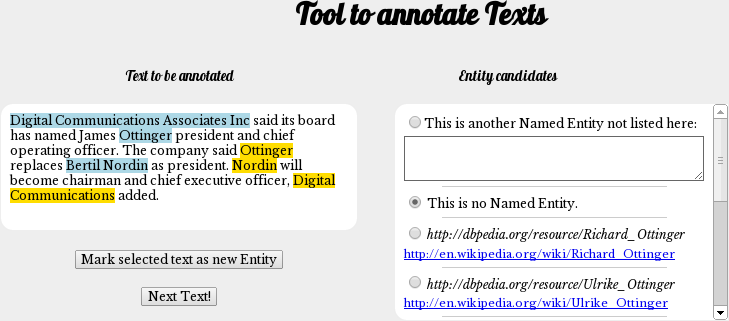
\includegraphics[width=\linewidth]{fig/qrtoolnew.png}
%    \caption{GUI of our annotation tool.}
%    \label{fig:qrtool}
%\end{figure*}

\subsection{Results}
\label{results}

\begin{table*}[hb!]
\centering
\caption{Evaluation of AGDISTIS against AIDA and DBpedia Spotlight. Bold indicates best \mbox{F-measure}.} \label{tab:evalold} 
\begin{tabular}{c ccc ccc c c}
\toprule
\textbf{Corpus}  & \multicolumn{6}{c}{\textbf{AGDISTIS}}	& \textbf{AIDA} & \textbf{Spotlight}\\\midrule
\textbf{$K$}& \multicolumn{3}{c}{{DBpedia}}& \multicolumn{3}{c}{{YAGO2}}	& {YAGO2} & {DBpedia}\\\midrule
				& \mbox{F-measure} 		& $\quad \sigma \quad $ & $\quad d \quad $ 	& \mbox{F-measure} & $\quad \sigma \quad $ & $\quad d \quad $ & \mbox{F-measure}  & \mbox{F-measure}\\
\cmidrule(r){2-4}  \cmidrule(r){5-7} \cmidrule{8-8} \cmidrule{9-9}
Reuters-21578	&  	\textbf{0.78}	&  			0.87		&  		2		& 	0.60	&  0.29		&  	3	&  	0.62		& 	0.56	\\
RSS-500 		&  	\textbf{0.75}	&  			0.76		&  		2		& 	0.53	&  0.82		&   2 	&  	0.60		& 	0.56	\\
\url{news.de} 	&  	\textbf{0.87}	&  			0.71		&  		2		& 	---		&   ---		&  ----	&  	----		& 	0.84	\\
AIDA-YAGO2	   	&  		0.73		&  			0.89		&  		2		& 	0.58	&  0.76		&   2 	&\textbf{0.83}	& 	0.57	\\
\bottomrule
\end{tabular}
\end{table*}

First, we evaluate AGDISTIS against AIDA and DBpedia Spotlight on three different knowledge bases using N3 corpora and the AIDA-YAGO2 corpus. 

AGDISTIS performs best on the \url{news.de} corpus, achieving a maximal 0.87 \mbox{F-measure} for $\sigma = 0.71$ and $d = 2$ (see Table~\ref{tab:evalold}).
Our approach also outperforms the state of the art on Reuters-21578 corpus (see Figure~\ref{fig:reuters}), where it reaches 0.78 \mbox{F-measure} for $\sigma = 0.87$ and $d = 2$.
Considering the AIDA-YAGO2 dataset AGDISTIS achieves an \mbox{F-measure} of 0.73 for $\sigma = 0.89$ and $d = 2$.
%In combination with the results on RSS-500, 
Our results suggest that $d=2, \sigma=0.82$ and using DBpedia as KB are a good setting for AGDISTIS and suffice to perform well. %The iteration of $\sigma$ between $0.7$ and $0.9$ can lead to an improvement of up to $6\%$ \mbox{F-measure}.
In the only case where $\sigma=0.29$ leads to better results (Reuters-21578 corpus), the setting $0.7<\sigma<0.9$ is only outperformed by 0.03 F-measure using YAGO as KB for AGDISTIS.

\begin{table}
    \centering
\caption{Performance of AGDISTIS, DBpedia Spotlight and TagMe 2 on four different datasets using micro F-measure (\textbf{F1}).}
\begin{tabular}[tb]{@{}lllll@{}}
\toprule
Dataset                            & Approach          & \textbf{F1-measure}             & \textbf{Precision} & \textbf{Recall} \\ \midrule
\multirow{3}{*}{\begin{minipage}{0.8in}\textbf{AIDA/CO-NLL-TestB}\end{minipage}} & TagMe 2           & 0.565          & 0.58      & 0.551  \\
                                   & DBpedia Spotlight & 0.341          & 0.308     & 0.384  \\
                                   & AGDISTIS          & \textbf{0.596} & \textbf{0.642}     & \textbf{0.556}  \\ \midrule
\multirow{3}{*}{\textbf{AQUAINT}}  & TagMe 2           & 0.457          & 0.412     & \textbf{0.514}  \\
                                   & DBpedia Spotlight & 0.26           & 0.178     & 0.48   \\
                                   & AGDISTIS          & \textbf{0.547} & \textbf{0.777}     & 0.422  \\\midrule
\multirow{3}{*}{\textbf{IITB}}     & TagMe 2           & 0.408          & 0.416     & 0.4    \\
                                   & DBpedia Spotlight & \textbf{0.46}  & 0.434     & \textbf{0.489}  \\
                                   & AGDISTIS          & 0.31           & \textbf{0.646}     & 0.204  \\\midrule
\multirow{3}{*}{\textbf{MSNBC}}    & TagMe 2           & 0.466          & 0.431     & 0.508  \\
                                   & DBpedia Spotlight & 0.331          & 0.317     & 0.347  \\
                                   & AGDISTIS          & \textbf{0.761} & \textbf{0.796}     & \textbf{0.729}  \\ \bottomrule
\end{tabular}
\label{tab:evalnew}
\end{table}

Second, we compared our approach with TagMe 2 and DBpedia using the datasets already implemented in the framework of Cornolti et al.
AGDISTIS has been setup to use a breadth-first search depth $d=2$ and a trigram similarity of $\sigma=0.82$.
All approaches used disambiguate w.r.t. the English DBpedia.
%TagMe 2 and DBpedia Spotlight are easily to test via web services while AIDA needs to be installed locally and run on a large machine. 
AIDA was ommitted from this evaluation because it has been shown to be outperformed by TagMe 2 in~\cite{cornolti} on the datasets we consider. 

AGDISTIS achieves \mbox{F-measures} between $0.31$ (IITB) and $0.76$ (MSNBC) (see Table~\ref{tab:evalnew}).
We outperform the currently best disambiguation framework, TagMe 2, on three out of four datasets by up to $29.5\%$ F-measure. 
Our poor performance on IITB is due to AGDISTIS not yet implementing a paragraph-wise disambiguation policy. 
By now, AGDISTIS performs disambiguation on full documents.
The large number of resources in the IITB documents thus lead to our approach generating very large disambiguation graphs.
The explosion of errors within these graphs results in an overall poor disambiguation.
We will address this drawback in future work by fitting AGDISTIS with a preprocessor able to extract paragraphs from input texts.
The local vector-space model used by Spotlight performs best in this setting. 

%\todo[inline]{Micha: the part "The iteration of $\sigma$ between $0.7$ and $0.9$ can lead to an improvement of up to $6\%$ \mbox{F-measure}" occurs two times. Remove one of them.}  
\begin{figure}[htb!]\centering
        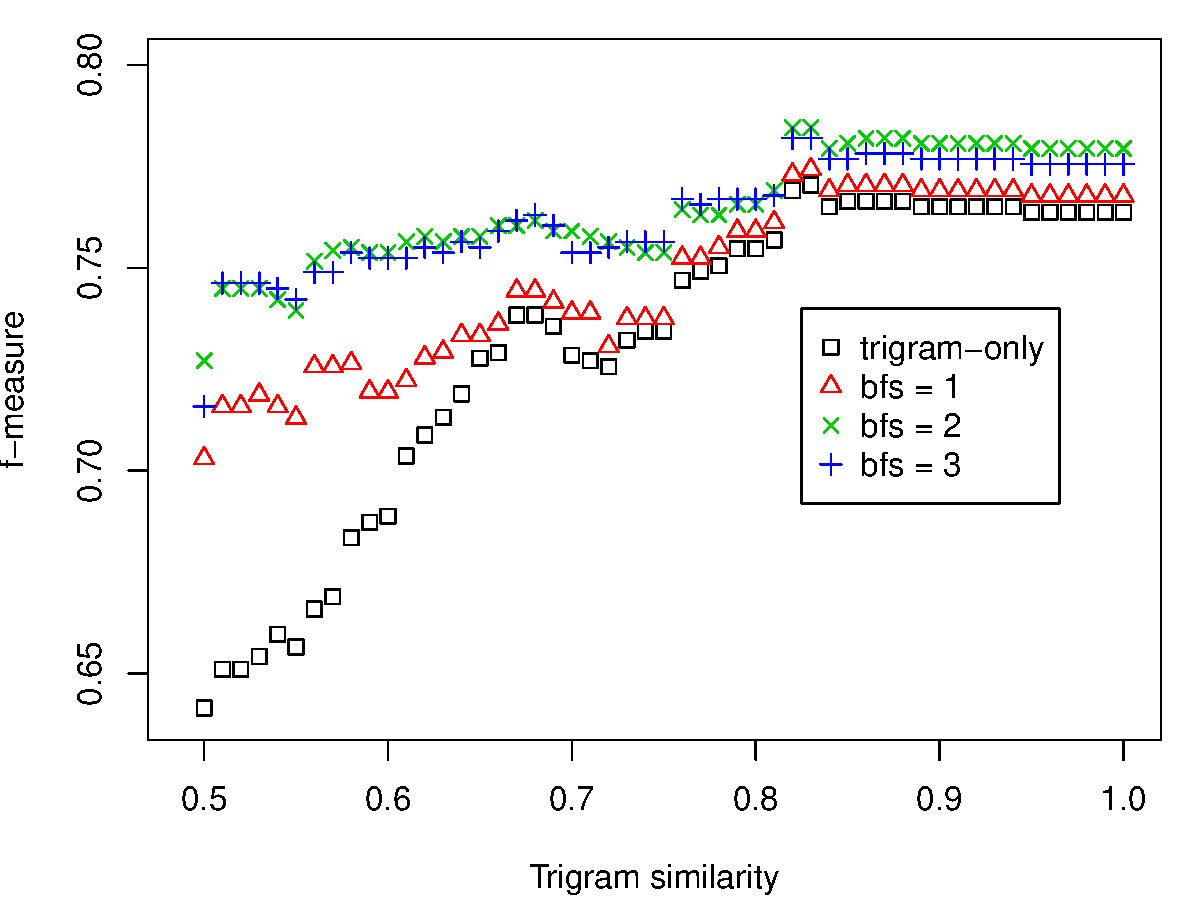
\includegraphics[width=0.9\linewidth]{chapter_three/unstructured_annotation/fig/reuters.pdf}
        %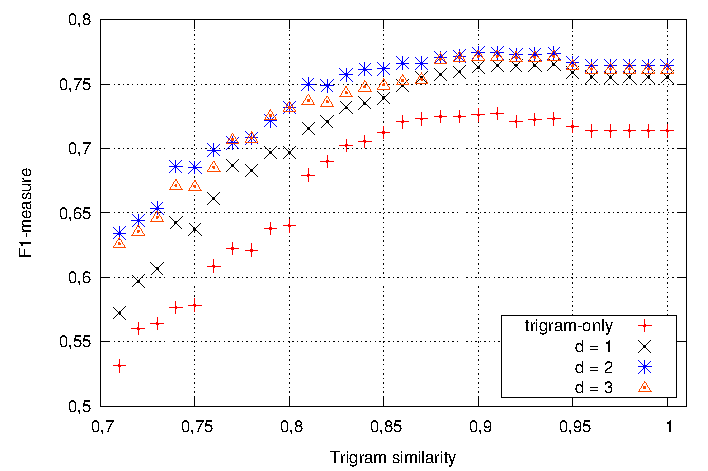
\includegraphics[width=0.9\linewidth]{fig/bfs_depth_diag.pdf}
    \caption{\mbox{F-measure} on the \textbf{Reuters-21578} corpus using DBpedia as KB.}  \label{fig:reuters}
\end{figure}

Delving deeper into AGDISTIS' results lead to the following insights:
(1) Varying the search depth $d$ does not significantly improve \mbox{F-measure} because within the underlying documents there are many similar named entities forming a shallow semantic background. However, using only string similarity measures ($d=0$) results in lower F-measure (see Figure \ref{fig:reuters}). % while the optimum has been found using $d=2$. %, see Figure~(\todo[inline]{here was a reference to a reuters figure}). 
(2) The expansion policy can have considerable knock-on effects: Either the first entity and its expansions are disambiguated correctly or the wrong disambiguation of the first entity leads to an avalanche of false results in a loss of $\approx 4\%$ accuracy.
%\todo[inline]{Micha: Why accuracy while you always talk about F-measure?}
(3) We observed a significant enhancement of AGDISTIS when adding surface forms to the labels of resources as explained in Section~\ref{choosing}.
Employing additional labels (such as surface forms gathered from Wikipedia) increased the \mbox{F-measure} of AGDISTIS by up to $4\%$. 
(5) Using $n=1,2,4$ as n-gram similarity has been proven to perform worse than using trigram similarity,\,i.e., $n=3$.
Our results suggest that $d=2$ while using DBpedia as KB is a good setting for AGDISTIS and suffice to perform well. 
The iteration of $\sigma$ between $0.7$ and $0.9$ can lead to an improvement of up to $6\%$ \mbox{F-measure} while $\sigma<0.7$ and $\sigma>0.9$ leads to a loss of F-measure.

Overall, our results suggest that $\sigma=0.82$ and $d=2$ is generally usable across datasets and knowledge bases leading to high quality results.\footnote{See also \url{http://139.18.2.164/rusbeck/agdistis/supplementary.pdf} and \url{http://139.18.2.164/rusbeck/agdistis/appendix.pdf}}
%Thus, in the following, we use $\sigma=0.82$. 

%This is done by selecting all resources as candidates that are such that the similarity of at least one of its labels and the 
%The best similarity thresholds $\sigma$ w.r.t. disambiguation \mbox{F-measure} achieved by our approach were determined empirically iterating $\sigma$ between 0 and 1 in steps of 0.01. 
%Setting $\sigma=0.82$ turned out to be the best threshold independent of the analysed dataset.%\footnote{See our project side for further evaluation \url{http://aksw.org/Projects/AGDISTIS}}% (cf. Section~\ref{eval}).
%as shown in Figure~\ref{fig:influenceOfSurfaceForms}.
%This explains the worse results achieved by AGDISTIS when using YAGO2 as KB. 

%\begin{figure}[htb!]\centering
%        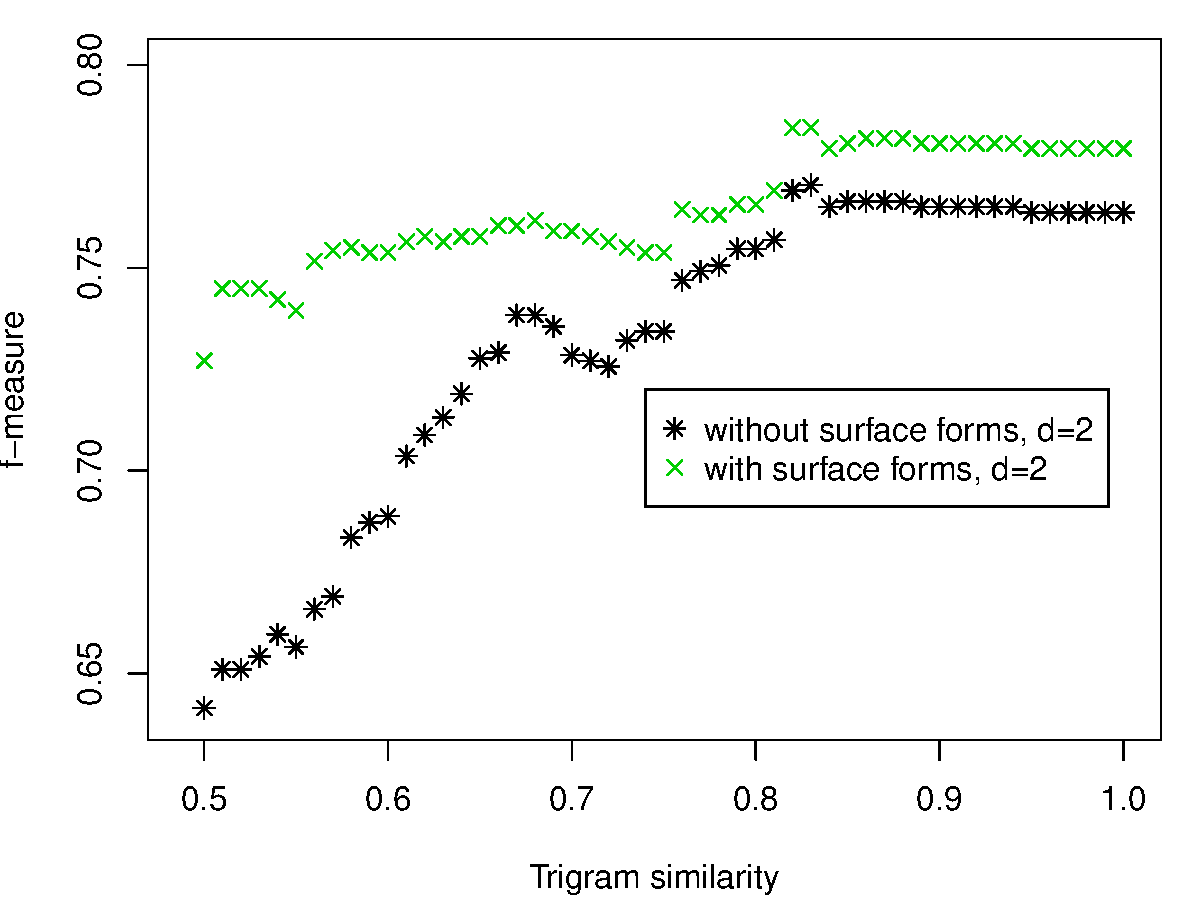
\includegraphics[width=0.9\linewidth]{fig/reutersWithoutSurfaceFormsAndBFS2.pdf}
        %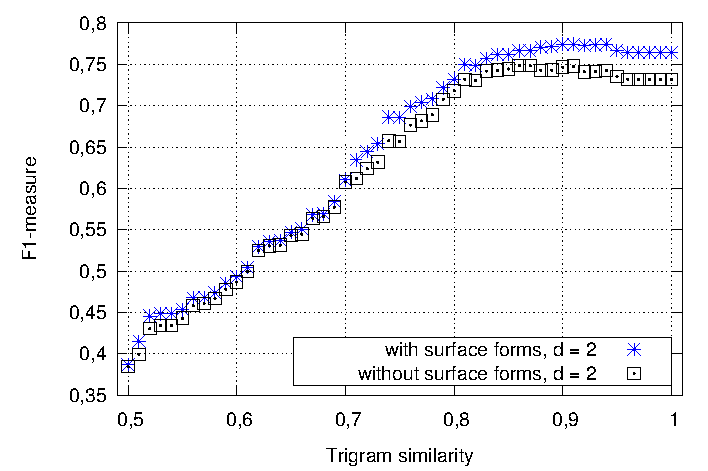
\includegraphics[width=0.9\linewidth]{fig/surface_forms_diag.pdf}
%    \caption{Influence of surface forms on the Reuters-21578 corpus and DBpedia as KB.}\label{fig:influenceOfSurfaceForms}
%\end{figure}
%\todo[inline]{@axel: not using any graph just trigram sim is worse than the rest}
% for AGDISTIS are worse since our approach could not make use of surface forms as explained above. %, redirects or disambiguation entities, as explained above.
%Yet, given that a 1-1 mapping exists between YAGO2 and DBpedia URIs, we will consider the results of DBpedia for AGDISTIS in the following comparisons with other tools.
%\todo[inline}]{AN:Formally wrong. Either a 1-1 mapping exists or it does not}
%If there is no 1-1 mapping, the result of the disambiguation is counted as \emph{false positive}, which then results in low \mbox{F-measures} using YAGO2 as KB.
%\todo{look at table caption please}


%\textbf{Comparison with AIDA.} 
%\todo[inline]{renew numbers}
%We compared our approach to AIDA by using the \textit{Cocktailparty configuration}\footnote{\url{https://github.com/yago-naga/aida}} (which is the recommended configuration for the framework) and applied the same restrictions that we used for AGDISTIS.
%The results of this evaluation on AIDA can be seen in Table~(\todo[inline]{here was a reference to the eval result}).
%Overall, AIDA performs well on arbitrary entities. 
%Yet, it is clearly outperformed by our approach on specific persons and organizations. 
%\todo[inline]{the statement above cant be seen in table 4, therefore we need to compare by type or clarify this sentence}
%In comparison to AIDA, AGDISTIS performs best on the Reuters-21578  where it surpasses AIDA by $\approx 0.16$ \mbox{F-measure}.
%Here AGDISTIS benefits from surface forms and its expansion policy.
%Furthermore, AGDISTIS outperforms AIDA with the RSS-500 corpus by $\approx 0.15$ \mbox{F-measure}.
%This corpus differs considerably from the Reuters-21578 corpus due to the small disambiguation contexts and graphs evolving from two named entities per text only.
%Note that AGDISTIS also outperforms AIDA for our overall default setting of $\sigma = 0.81$, apart from the result on the AIDA-YAGO2 corpus.
%AIDA could not be run on the \url{news.de} corpus as it can only deal with English.
%Here, the \emph{language-independence} of AGDISTIS provides a significant improvement of the state of the art.
%AIDA performs better on AIDA-YAGO2 achieving an \mbox{F-measure} of 0.83 due to the large contexts of the documents (see Table~(\todo[inline]{here was a reference to a data table})).
%This is clearly due to AGDISTIS being tuned towards smaller contexts since these are more common in WND, see Table~(\todo[inline]{here was a reference to a data table}).
%In particular, the AIDA-YAGO2 corpus contains many sport teams from cities and countries like \texttt{Barcelona} where AGDISTIS identifies \texttt{dbr:Barcelona} and \texttt{dbr:FC\_Barcelona} as resources. Since \texttt{dbr:Barcelona} has a higher authoritative score than \texttt{dbr:FC\_Barcelona}, AGDISTIS' disambiguation results in a \emph{false positive} in this particular case.
%As shown in Table~\ref{eval} using YAGO2 leads to worse results since AGDISTIS (in contrast to AIDA) does not possess surface forms for YAGO2.
%\todo[inline]{No appendiy, how to solve this?}

%\textbf{Comparison with DBpedia Spotlight.}
%\todo[inline]{renew the numbers}
%In order to compare DBpedia Spotlight with AGDISTIS Cornolti et al.~\cite{cornolti} used Spotlight's Web services.\footnote{\url{https://github.com/dbpedia-spotlight/dbpedia-spotlight/wiki/Web-service}}

%The results of the evaluation are shown in Table~\ref{tab:eval}.
%Spotlight performs best on the \url{news.de} dataset (\mbox{F-measure} = 0.84) and worst on the Reuters-21578 dataset (\mbox{F-measure} = 0.56), Table~(\todo[inline]{here was a reference to the eval result}).
%This is possibly due to the datasets age of over 20 years and missing historic data in DBpedia.
%When evaluated against the AIDA-YAGO2 corpus Spotlight achieves a \mbox{F-measure} of 0.57.
%Using the RSS-500 dataset Spotlight is only able to generate a \mbox{F-measure} of 0.56.
%\todo[inline]{renew the number}
%AGDISTIS outperforms Spotlight by at least $\approx 0.15$ \mbox{F-measure}. % using DBpedia as KB. on each English dataset.

%AGDISTIS performs better on two of the datasets and is even usable for the German dataset as it is agnostic towards the language of the used KB.
%As can be seen in Figure \ref{fig:relation} the number of entities per text is an important criteria for disambiguation.

%\textbf{Run time analysis.}
%On average AGDISTIS is more time-efficient than AIDA with respect to the best %corresponding configuration.
%While AGDISTIS finished its computation on Reuters-21578 corpus in 549\,seconds (s), AIDA needed more than twice as much time,\,i.e., 1,296\,s.
%This behavior can also be seen on the short documents of the RSS-500 dataset, where AIDA needed 4,919\,s and our approach only 623\,s.
%Moreover, AGDISTIS outperforms AIDA with 3,946\,s to 51,435\,s run time on the AIDA-YAGO2 corpus.
%\todo[inline]{is not comparable anymore since we needed to run it in the cloud}
%Details can be found on the project website.

\section{Conclusion}
\label{sec:conclusion}
%\todo[inline]{Micha: AIDA is missing in the conclusion.}
We presented AGDISTIS a novel named entity disambiguation that combines the scalable HITS algorithm and breadth-first search with linguistic heuristics.
Our approach outperforms the state-of-the-art algorithms TagMe 2, AIDA and DBpedia Spotlight while remaining quadratic in its time complexity. 
Moreover, our evaluation suggests that while the approach performs well in and of itself, it can benefit from being presented with more linguistic information such as surface forms. 
%Furthermore, we measured the effect of evolving the structure of the underlying knowledge base.
%We observed the significance of properties on the \mbox{F-measure} performance of our system.
%Our results suggest that only a few RDF properties contribute significantly to enhancing the performance of AGDISTIS.
We see this work as the first step in a larger research agenda.
Based on AGDISTIS, we aim to develop a new paradigm for realizing NLP services which employ community-generated, multilingual and evolving Linked Open Data background knowledge.
Other than most work, which mainly uses statistics and heuristics, we aim to truly exploit the graph structure and semantics of the background knowledge.

Since AGDISTIS is agnostic of the underlying knowledge base and language-independent, it can profit from growing KBs as well as multilingual Linked Data.
In the future, we will thus extend AGDISTIS by using different underlying KBs and even more domain-specific datasets.
An evaluation of Babelfy against our approach will be published on the project website.
Moreover, we will implement a sliding-window-based extension of AGDISTIS to account for large amounts of entities per document.
%A novel avenue of research would be combining AGDISTIS with topic modelling~\cite{Blei:2003:LDA:944919.944937}. Preliminary experiments in this direction show that we can improve the F-measure of our approach by at least 1\% on all datasets.
%In the future we intend to look for larger, more domain-specific and even more insightful disambiguation datasets to refine and test AGDISTIS.
%Moreover, a deeper evaluation of ontology structures towards disambiguation accuracies is needed.
%Answering those research questions will expose possible performance-enhancing extensions.
%





\section{Multilingual Disambiguation of Named Entities Using Linked Data}




One key step towards extracting structured data from unstructured data sources is the disambiguation of entities.
With AGDISTIS, we provide a time-efficient, state-of-the-art, knowledge-base-agnostic and multilingual framework for the disambiguation of RDF resources.
The aim of this demo is to present the English, German and Chinese version of our framework based on DBpedia.
We show the results of the framework on texts pertaining to manifold domains including news, sports, automobiles and e-commerce.
We also summarize the results of the evaluation of AGDISTIS on several languages.

\section{Introduction}
A significant portion of the information on the Web is still only available in textual format. 
Addressing this information gap between the Document Web and the Data Web requires amongst others the extraction of entities and relations between these entities from text.
One key step during this processing is the disambiguation of entities (also known as entity linking).
The AGDISTIS framework~\cite{agdistis_iswc} (which will also be presented at this conference) addresses two of the major drawbacks of current entity linking frameworks~\cite{TagMe2,spotlight,babelfy}: time complexity and accuracy.
With AGDISTIS, we have developed a framework that achieves polynomial time complexity and outperforms the state of the art w.r.t. accuracy.
The framework is knowledge-base-agnostic (i.e., it can be deployed on any knowledge base) and is also language-independent.
In this demo, we will present AGDISTIS deployed on three different languages (English, German and Chinese) and three different knowledge bases (DBpedia, the German DBpedia and the Chinese DBpedia).
To the best of our knowledge, we therewith provide the first Chinese instantiation of entity linking to DBpedia.
We will also demonstrate the AGDISTIS web services endpoints for German, English and Chinese disambiguation and show how data can be sent to the endpoints.
Moreover, the output format of AGDISTIS will be explained.
An online version of the demo is available at \url{http://agdistis.aksw.org/demo}.
%In the following, we present the two ways of approaching AGDISTIS, architecture and workflow.

 
 
\section{Demonstration}
Within our demonstration, we aim to show how AGDISTIS can be used by non-expert as well as expert users.
For non-experts, we provide a graphical user interface (GUI).
Experts can choose to use the REST interfaces provided by the tool or use a Java snippet to call the REST interface.
The whole of this functionality, which will be described in more details in the following sections, will also be demonstrated at the conference.

\subsection{AGDISTIS for non-expert users}
A screenshot of the AGDISTIS GUI is shown in Figure~\ref{fig:gui}.
This GUI supports the following workflow.

\begin{figure}
\centering
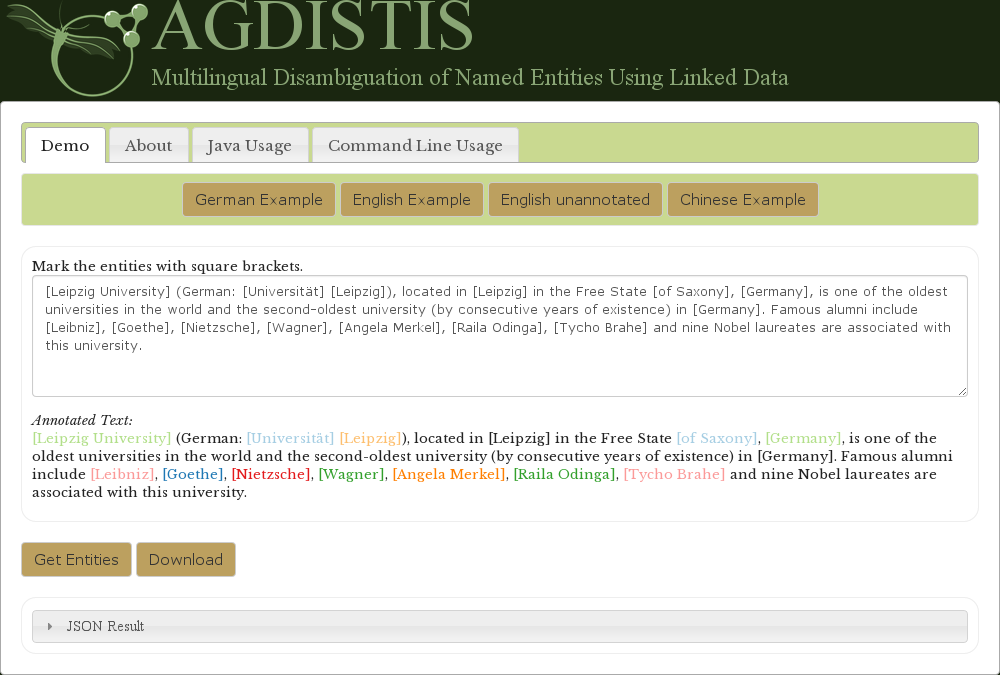
\includegraphics[width=\textwidth]{chapter_three/unstructured_annotation/fig/GUI.png}
\caption{Screenshot of the demo with an English example which is already annotated.}
\label{fig:gui}
\end{figure}

\noindent\textbf{Entity Recognition}
After typing or pasting text into the input field, users can choose between either annotating the entities manually or having the entities detected automatically.
In the first case, the labels of the entities are to be marked by using square brackets (see central panel of Figure~\ref{fig:gui}).
In the case of an automatic annotation, we send the text to the FOX framework, which has been shown to outperform the state of the art in~\cite{FOX}.
%In our current implemen
%Since there is no multilingual NER tool available, an automatic annotation of entities works only for English texts.
We will demonstrate this feature by using both manually pre-annotated text and text without annotations in our examples (see upper bar of Figure~\ref{fig:gui}).
Moreover, we will allow the crowd to enter arbitrary texts that pertain to their domain of interest.

\noindent\textbf{Automatic Language Detection}
Once the user has set which entities are to be disambiguated, the marked-up text is sent to the language detection module based on~\cite{nakatani2010langdetect}.
We chose this library because it is both precise ($>99\%$ precision) and time-efficient.
If the input is detected to belong to one of the languages we support (i.e., German, Chinese, English), then we forward the input to a dedicated AGDISTIS instance for this given language.
In all other cases, an error message is shown to the user, pointing towards the language at hand not being supported.
The main advantage of this approach is that the user does not need to select the language in which the text is explicated manually, thus leading to an improved user experience. 
We will demonstrate this feature by entering text in different languages (German, English, French, Chinese, etc.) and presenting the output of the framework for each of these test cases.

\noindent\textbf{Entity Linking} 
This is the most important step of the whole workflow.
The annotated text is forwarded to the corresponding language-specific deployment of AGDISTIS, of which each relies on a language-specific version of DBpedia 3.9. 
The approach underlying AGDISTIS~\cite{agdistis_iswc} is language-independent and combines breadth-first search and the well-known HITS algorithm. 
In addition, string similarity measures and label expansion heuristics are used to account for typos and morphological variations in naming.
Moreover, Wikipedia-specific surface forms for resources can be used. 

\noindent\textbf{Output}
Within the demo the annotated text is shown below the input field where disambiguated entities are colored to highlight them. 
While hovering a highlighted entity the disambiguated URI is shown.
We will demonstrate the output of the entity linking by using the examples shown in the upper part of Figure~\ref{fig:gui}. 
The output of the system will be shown both in a HTML version and made available as a download in JSON. 
Moreover, we will allow interested participants to enter their own examples and view the output of the tool.

\subsection{AGDISTIS for expert users}

To support different languages we set up a REST URI for each of the language versions.
%those\footnote{\url{http://139.18.2.164:8080/AGDISTIS_DE}}\footnote{\url{http://139.18.2.164:8080/AGDISTIS_ZH}}\footnote{\url{http://139.18.2.164:8080/AGDISTIS}}.
Each of these endpoints understands two mandatory parameters: (1) \texttt{text} which is an UTF-8 and URL encoded string with entities annotated with XML-tag \texttt{<entity>} and (2) \texttt{type='agdistis'} to disambiguate with the AGDISTIS algorithm.
In the future, several wrappers will be implemented to use different entity linking algorithms for comparison.
Following, a CURL\footnote{\url{http://curl.haxx.se/}} snippet shows how to address the web service, see also \url{http://agdistis.aksw.org}:
\begin{verbatim}
curl --data-urlencode "text='<entity>Barack Obama</entity> arrives 
in <entity>Washington, D.C.</entity>.'" -d type='agdistis' 
{AGDISTIS URL}/AGDISTIS
\end{verbatim}

\section{Evaluation}
\textbf{English and German Evaluation.} AGDISTIS has been evaluated on 8 different datasets from diverse domains such as news, sports or buisiness reports.
For English datasets AGDISTIS is able to outperform the currently best disambiguation framework, TagMe2, on three out of four datasets by up to 29.5\% F-measure. 
Considering the only German dataset available for named entity disambiguation, i.e., \url{news.de}~\cite{n3}, we are able to outperform the only competitor DBpedia Spotlight by 3\% F-measure.


\noindent \textbf{Chinese Evaluation.} We evaluated the Chinese version of AGDISTIS within a question answering setting. 
To this end, we used the multilingual benchmark provided in QALD-4\footnote{\url{http://greententacle.techfak.uni-bielefeld.de/~cunger/qald}}. 
Since the Chinese language is not supported, we extended the QALD-4 benchmark by translating the English questions to Chinese and inserted the named entity links manually.
The accuracies achieved by AGDISTIS for the train and test datasets are 65\% and 70\% respectively. 
%We also performed a fully automatic evaluation by using the Chinese segmentation and named-entity recognition algorithms provided by LTP-Cloud\footnote{\url{http://www.ltp-cloud.com/}}. 
%The accuracies sank to 32\% and 38\%.
%These results indicate the need for better resources for Entity Recognition in Chinese.
\section{Conclusion}
We presented the demo of AGDISTIS for three different languages on three different DBpedia-based knowledge bases.
In future work, we aim to create a single-server multilingual version of the framework that will intrinsically support several languages at the same time.
To this end, we will use a graph merging algorithm to combine the different versions of DBpedia to a single graph.
The disambiguation steps will then be carried out on this unique graph.
%expand different knowledge base and 
%a full dbpedia supported multilingual version









\section{How the Chinese version was generated}
\label{sec:chinese}

The key to extend AGDISTIS to support a new language is to provide the needed RDF data for this particular language, especially \texttt{rdf:type} information. 
%However, the latest available Linked Data --- DBpedia 3.9 --- has no such information for Chinese. 
%Therefore, we created triples containing \texttt{rdf:type} as predicate by translating the English ones to Chinese. 
%Specifically, we use inter-language links extracted by DBpedia 
%\footnote{Available from \url{http://wiki.dbpedia.org/Downloads39\#inter-language-links}}, in which a English resource is represented in different other languages. 
%An English-Chinese pair of phrases for each resource is extracted using the following regular expression\footnote{{\it zh} is the language code for Chinese.}:
%\begin{verbatim}
%``$\langle http://dbpedia\backslash.org/resource/(.*)\rangle\backslash s*\langle.*\rangle \backslash s*\langle http://zh.dbpedia.org/resource/(.*)\rangle\backslash s*.$"
%\end{verbatim}
%, resulting a phrase table with 420,047 English-Chinese pairs.

%For each rdf:type triple in the English DBpedia, if the name of the subject appears in the phrase table, it is mapped to Chinese according to the phrase table. In this way, a total of 1,234,783 triples are extrated for Chinese.

%Both the data stored in a Lucene 4.5.1 Index and the phrase table can be found at \url{http://139.18.2.164/rusbeck/}.

%\subsection{Accuracy results of the Chinese version}
%In this section, we will introduce a new Chinese benchmark and the evaluation results.

\subsubsection{Chinese Benchmark}

To evaluate the Chinese version of AGISTIS, a Chinese benchmark is created in the context of question answering because the disambiguation of named entities is a key step to answer a natural language question based on linked data. 

A first try is to adopt the multilingual benchmark provided in QALD-4~\cite{qald4} for question answering. Unfortunately, the Chinese language is not supported. Therefore, we extended the QALD-4 benchmark by translating the English questions to Chinese and annotated the named entity links manually. The links in the given SPARQL queries for the questions are assumed to be the correct links for the English entities, which are adapted to the Chinese links by hand. It results in 200 Chinese questions in the training data and 50 ones in the test data, with an average of 0.9 named entity links per question. The Chinese benchmark is available at \url{https://github.com/wencanluo/DBpediaQA/tree/master/benchmark/qald4}.

\subsubsection{Results}
We first report the disambiguation accuracies by assuming the named entities are given. It allows a fair comparison to other disambiguation algorithms because named entity disambiguation performance is highly depended on named-entity recognition results. The accuracy is measured at a sentence level by assuming a correct disambiguation should recognize and link all the entities in a sentence, which is essential for further steps in question answering. The accuracies for the training and testing are 65\% and 70\% respectively. 

We also performance a fully automatic evaluation by using the Chinese segmentation and named-entity recognition algorithms provided by LTP-Cloud\footnote{\url{http://www.ltp-cloud.com/}}. 
The accuracies are 32\% and 38\%.

architecture, what are the main steps

GOAL is to provide entity linking results to several languages which are show on the website and downloadable as JSON

1 we will present and explain how AGDISTIS works and how multilinguality is achieved

2 Users can try different inputs at the demo station and tell us, what quality they expect and which languages they want

3 finally we will show how the results can be downloaded or seen online and how the annotation of more or less entities changes the behaviour of AGDISTIS

benchmarks will be shown as well and people will be invited to use our for free endpoint for their projects so we can store the use case data and improve our approach similar to the feedback API of spotlight and fox



%\usepackage[table,xcdraw]{xcolor}
%\usepackage{booktabs}
%\usepackage{multirow}

%\usepackage{listings} 
\lstset{
  basicstyle=\footnotesize\ttfamily,
  breaklines=true,
  captionpos=b,                    % sets the caption-position to bottom
  frame=single,
  %morecomment=[s][\color{blue}]{<}{>},
  morecomment=[s][\color{red}]{"}{"},
  numbers=left,
  numbersep=5pt,
  numberstyle=\tiny,
  stringstyle=\tiny
}

%\DeclareUnicodeCharacter{0177}{\p1}


\chapter{Type Annotation on Unstructured Texts}
%\title{CETUS -- A Baseline Approach to Type Extraction}
%\author{
%Michael Röder\inst{1} \and
%Ricardo Usbeck\inst{1} \and
%Axel-Cyrille Ngonga Ngomo\inst{1}
%}
%\institute{
%University of Leipzig, Germany\\\email{\{roeder,usbeck,ngonga\}@informatik.uni-leipzig.de}
%}


%\begin{abstract}
The concurrent growth of the Document Web and the Data Web demands accurate information extraction tools to bridge the gap between the two.
In particular, the extraction of knowledge on real-world entities is indispensable to populate knowledge bases on the Web of Data. 
Here, we focus on the recognition of types for entities to populate knowledge bases and enable subsequent knowledge extraction steps.
We present CETUS, a baseline approach to entity type extraction tool.
CETUS is based on a three-step pipeline comprising i) offline, knowledge-driven type pattern extraction from natural-language corpora based on grammar-rules, ii) an analysis of input text to extract types and iii) the mapping of the extracted type evidence to a subset of the DOLCE+DnS Ultra Lite ontology classes.
We implement and compare two approaches for the third step using the YAGO ontology as well as the FOX entity recognition tool.
%\end{abstract}


\section{Introduction}

Both the Document and the Data Web grow continuously. This is a mixed blessing, as the two forms of the Web grow concurrently and most commonly contain different forms of information. Modern information systems must thus bridge this gap to allow a holistic access to the Web. One way to bridge the gap between the two forms of the Web is the extraction of structured data from the growing amount of unstructured information on the Document Web. 
While extracting structured data from unstructured data allows the development of powerful information system, it also requires high-quality knowledge extraction tool chains to lead to useful results. 
However, standard document processing pipelines miss the opportunity to gain insights from semantic entities novel to the underlying knowledge base (KB). 
That is, most known tool chains recognize entities based on linguistic models and link them to a KB or null if they are emerging entities. 
So far, linking novel entities has only been the concern of a few approaches~\cite{AIDA,AGDISTIS_ISWC}.
Consequently, extracting type information for emerging and existing entities is a novel research avenue so far only tackled by the TAC KBP Entity Linking challenge 2014\footnote{\url{http://nlp.cs.rpi.edu/kbp/2014/}}, the Micropost workshop series\footnote{\url{http://www.scc.lancs.ac.uk/microposts2015/}} and the OKE challenge 2015\footnote{\url{http://2015.eswc-conferences.org/important-dates/call-OKEC}}.

In this article, we present CETUS, a novel pattern based entity type extraction tool for identifying the type of a given entity inside a given text and linking this type to a KB, i.e., to the subset of the DOLCE+DnS Ultra Lite ontology classes\footnote{\url{http://www.ontologydesignpatterns.org/ont/dul/DUL.owl}}.
Here the subset refers to \texttt{dul:Person}, \texttt{dul:Place}, \texttt{dul:Organization} and \texttt{dul:Role}\footnote{Throughout this paper, we use the prefix \texttt{dul} for \url{http://www.ontologydesignpatterns.org/ont/dul/DUL.owl}.}.
CETUS is a fast and easy to implement baseline approach to path a way to novel research insights.
CETUS' pipeline is divided into three subsequent parts: i) an a-priori pattern extraction, ii) a grammar-based analysis of the input document and iii) a mapping the type evidence to the DOLCE+DnS Ultra Lite classes. 
CETUS implements two approaches for the third step using the YAGO ontology as well as the FOX entity recognition tool.
We will explain these parts in detail in the Sections~\ref{sec:patternExt},~\ref{sec:docAnalysis},~\ref{sec:linkingyago} and~\ref{sec:typeLinking} respectively, before we conclude in Section~\ref{cha321:sec:conclusion}. The source code of CETUS can be found at \url{https://github.com/AKSW/Cetus}.

\section{Related Work}

Next to the above mentioned challenges about entity linking, several tools have been introduced with the ability to type entities, e.g., FOX~\cite{FOX}.
However, these tools differ in two major aspects compared to CETUS.
First, existing tools contain only very general type hierarchies while our approach generates novel and fine grained classes, see Section~\ref{sec:docAnalysis}.
Second, CETUS is the first tool to mark the part of a given document that contains the type evidence, i.e., a string indicating the choosen type.
Thus, there is a clear difference between the entity typing and the type extraction tasks.
To the best of our knowledge, CETUS is the first approach to tackle the type extraction task.

%\todo[inline]{Cite BOA, since it is pattern based, too, but made for relation extraction.}
Our approach is mainly based on patterns and is inspired by  Hearst Patterns~\cite{Hearst1992}.
Those patterns match text parts describing hyponym relations between two nouns.
In difference to our patterns, the Hearst Patterns have been extracted from a large corpus using a bootstrapping approach.
As described in Section~\ref{sec:patternExt}, our patterns are defined for matching text parts describing the type relation of a given entity and have been created manually during an iterative, incremental process.

\section{Pattern Extraction}
\label{sec:patternExt}

The patterns used for identifying the type of an entity inside a document, are generated semi-automatically in an iterative manner.
First, CETUS identifies phrases containing entities and their types in a given document corpus (here we use the DBpedia 2014 abstracts) and extracts them.
After sorting these phrases according to the string in between the entity and its type, we analyze them and create the patterns in an incremental process.
The progress of our pattern extraction is measured by the amount of phrases that are covered by our patterns.
In the following, these steps are described in more detail.

\subsection{Sentence Part Extraction}

For extracting the phrases containing entities and their types, we used the abstracts of the English DBpedia 2014 abstracts dump file.
Every abstract describes the entity it belongs to and, thus, contains the label of the entity and its type.
We assume, abstracts are written properly and thus contain both information.

First, CETUS preprocesses each abstract individually.
Our approach removes the text written in brackets, e.g., pronunciations.
Afterwards, we use the Stanford Deterministic Coreference Resolution System~\cite{Lee2013} to replace pronouns with their coreferenced words, e.g., \emph{He studied physics} with \emph{Albert Einstein studied physics}.
The last step of the preprocessing is the splitting of the abstracts into single sentences.

Second, sentences containing the entity label and at least one label of one of its types (\texttt{rdf:type}) are processed further.
CETUS extracts the part of the sentence between the entity label and the type label and stores additionally the words, their lemmas and part-of-speech tags of the extracted phrase.

After analysing all abstracts, CETUS counts the different phrases.
Table~\ref{tab:extParts} shows examples of extracted phrases and their counts how often they have been found inside the English DBpedia.
The words inside these parts are encoded as \texttt{<word>\_<lemma>\_<pos-tag>}.

Delving into the extracted phrases reveals insights into the structure of entity type descriptions in DBpedia abstracts.
It can be seen that the formulation "\texttt{<entity>} \emph{is a} \texttt{<type>}" occurs most often.
%The second most common formulation is nearly the only one in our list, in which the type precedes the entity.
The second most common formulation uses a type preceding the entity and is listed as the second example in table~\ref{tab:extParts}.
The third example is a variant of the first one containing the determine "an" instead of "a".
The fourth example shows that some abstracts contain more complex formulations like "\texttt{<entity>} \emph{is a} \texttt{<type>} \emph{of} \texttt{<type>}" while the last example contains an additional adjective that was not a part of the types label, i.e., "flowering".

\begin{table}
\centering
\begin{tabular}{lp{5mm}r}
 \toprule
 \multicolumn{1}{c}{\textbf{Extracted phrase}} && \multicolumn{1}{c}{\textbf{Count}} \\
 \midrule
 \texttt{<entity> is\_be\_vbz a\_a\_dt <type>} && 242\,806 \\
 \texttt{<type> <entity>} && 107\,082 \\
 \texttt{<entity> is\_be\_vbz an\_an\_dt <type>} && 12\,981 \\
 \texttt{<entity> is\_be\_vbz a\_a\_dt species\_species\_n1 of\_of\_pp-f <type>} && 12\,554 \\
 \texttt{<entity> is\_be\_vbz a\_a\_dt species\_species\_n1} && \multirow{2}{*}{4\,069} \\ 
 \qquad\qquad\ \ \texttt{of\_of\_pp-f flowering\_flower\_j-vvg <type>} && \\
 \bottomrule
\end{tabular}
\caption{Examples of sentence parts found between an entity and its type.}
\label{tab:extParts}
\end{table}

\subsection{Grammar Construction}
\label{sec:grammar}

The aim of creating a grammar is to generate a parser that is able to identify the part of a sentence describing an entities type given the position of the entity inside the sentence.
For generating a parser based on our grammar, we are using the ANTLR4 library\footnote{\url{http://www.antlr.org/}}.

Our grammar is based on the following assumptions:
\begin{enumerate}
\item A sentence contains an entity and a type. Otherwise the sentence is not part of our grammar language.
\item A type must contain a noun, but can contain additional words that are specifying the meaning of the noun, e.g., adjectives.
%Note, that the type is not a noun phrase!
\end{enumerate}

The first assumption simplifies the task of defining a grammar since we can focus on the sentences that are important for our task and ignore all others.
The second assumption contains the definition of a type surface form.
It might seem to be contradictory w.r.t. the last example of Table~\ref{tab:extParts} but for the extraction it is important that we extract all words that \emph{could} be part of the types surface form.
Following this assumptions, we can define a type inside the grammar with the rule in Listing~\ref{lst:typeRule}.

\begin{figure}
\begin{lstlisting}[label=lst:typeRule,caption=The grammar rule defining a type surface form.]{typeRule}
type : (ADJECTIVE|VERB|ADVERB)* FOREIGN? NOUN+;
\end{lstlisting}
\end{figure}

A surface form of a type can contain a number of adjectives, verbs or adverbs as well as a foreign word, e.g., the latin word "sub".
Additionally, a type has one or more nouns.

As mentioned above, the construction of the grammar is designed to be an iterative, incremental, self-improving process.
We start with the simple \emph{is-a} pattern that matches the most common phrase "\texttt{<entity>} \emph{is a} \texttt{<type>}". 
The definition of this pattern is shown in Listing~\ref{lst:firstIsARule}.
\begin{figure}
\begin{lstlisting}[label=lst:firstIsARule,caption=First simple version of the \emph{is-a} pattern. \texttt{ENTITY} is a marking for the entities position.]{firstIsARule}
is_a_pattern : ENTITY is_is_vbz a_a_dt type;
\end{lstlisting}
\end{figure}

With this simple grammar, we try to match all phrases extracted beforehand and create a list containing all those phrases that have not been matched so far.
Using this list, we extend our grammar to match other phrases.
In our example, we extend the simple \emph{is-a} pattern towards matching different temporal forms of the verb "be" and different determiners, e.g., "a" and "an", see Listing~\ref{lst:secondIsARule}.

\begin{figure}
\begin{lstlisting}[label=lst:secondIsARule,caption=Extended version of the \emph{is-a} pattern.]{secondIsARule}
is_a_pattern : ENTITY FORM_OF_BE DETERMINER type_with_dt;

FORM_OF_BE : ~[ \t\r\n]+ '_be_v' ~[ \t\r\n]*;
DETERMINER : ~[ \t\r\n]+ '_' ~[ \t\r\n]+ '_d' ~[ \t\r\n]*;
\end{lstlisting}
\end{figure}

With this iterative, incremental process, we further extended the grammar until we covered more than 90\% of the extracted phrases.\footnote{The complete grammar can be found in the projects source code repository.}

%\subsection{Example Patterns}

%\todo[inline]{Should we keep this section or delete it?}

%\begin{figure}
%\begin{lstlisting}[label=lst:allPatternRules,caption=The grammar rules for finding a type surface form.]{allPatternRules}
%sentence : WORD* ENTITY (COMMA (WORD|POINT|COMMA|COLON)+ COMMA)? type_after_entity_pattern (WORD|POINT|COMMA|COLON)*
%| WORD* type_in_front_of_entity ENTITY WORD*;
%
%type_after_entity_pattern : is_a_type_of_pattern
%| is_a_pattern
%| type_with_dt ;
%
%is_a_pattern : FORM_OF_BE type_with_dt (((COMMA? AND) | COMMA) type_with_dt)*;
%is_a_type_of_pattern : FORM_OF_BE type_with_dt OF type_with_dt;
%
%type_in_front_of_entity : type_with_dt (OF|COMMA|COLON)?;
%
%type_with_dt : DETERMINER? nr_or_crd? type;
%nr_or_crd : NUMBER | CARDINAL_NUMBER;
%\end{lstlisting}
%\end{figure}

\section{Type Extraction}
\label{sec:docAnalysis}

The pattern-based type extraction can be separated into two steps.
The first step extracts type evidence strings from the text, while the second step creates a local type hierarchy based on the extracted string.
Following, we describe both steps in more detail.

\subsection{Type String Extraction}

To identify the type evidence string for a certain entity, CETUS extracts the string containing the type of a given entity from a given text using the grammar from above.
Let us assume the following running example: CETUS processes the document as input with "Albert Einstein" marked as entity.

\begin{center}
\emph{In 1921, \textbf{Albert Einstein} got the Nobel Prize in Physics. He was a German-born theoretical physicist.}
\end{center}

First, the Stanford Deterministic Coreference Resolution System is applied to replace the pronoun of the second sentence by "Albert Einstein".

\begin{center}
\emph{In 1921, \textbf{Albert Einstein} got the Nobel Prize in Physics. \textbf{Albert Einstein} was a German-born theoretical physicist.}
\end{center}

After that, the text is split into sentences and the surface form of the entity is replaced by a placeholder.

\begin{center}
\emph{In 1921, \textbf{ENTITY} got the Nobel Prize in Physics.}

\emph{\textbf{ENTITY} was a German-born theoretical physicist.}
\end{center}

A parser based on the grammar from Section~\ref{sec:grammar} is applied to every sentence.
While the first sentence is identified as not contained in the language of the grammar, the second sentence is identified to be in the language.
Moreover, the parser identifies "German-born theoretical physicist" as evidence type string.

\subsection{Local Type Hierarchy}

Based on the extracted evidence type string, CETUS creates a type hierarchy and links the given entity to the hierarchy.
The type hierarchy comprises classes that are generated automatically from the extracted string based on the second assumption of Section~\ref{sec:grammar}.
Each class is generated by concatenating the words found in the extracted string using camel case.
After a class has been created, the first word is removed and the next class is created.
Every following class is a super class of the classes generated before.
Finally, the entity is connected to all generated classes.

For our example, three classes would be generated and linked to the entity as shown in Listing~\ref{lst:localHierarchy}\footnote{The \texttt{rdfs} prefix stands for \url{http://www.w3.org/2000/01/rdf-schema\#} while the prefix \texttt{ex} could stay for every user defined vocabulary, e.g., \url{http://example.com/}.}.

\begin{figure}
\centering
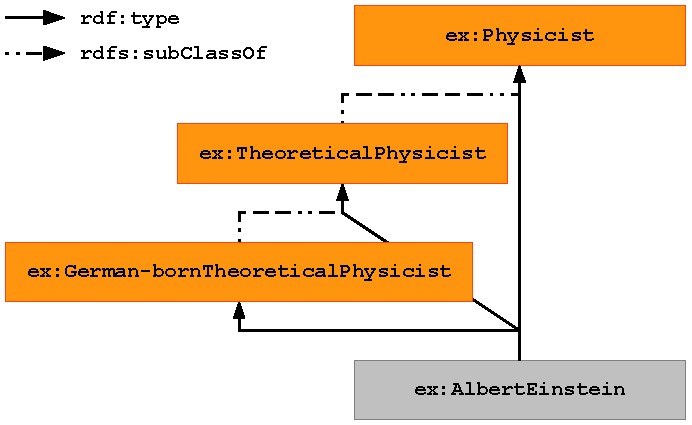
\includegraphics[scale=0.8]{chapter_three/unstructured_annotation/fig/localHierarchy.pdf}
\caption{Schema of the generated local hierarchy of the example.}
\label{fig:localHierarchy}
\end{figure}

\begin{figure}
\begin{lstlisting}[label=lst:localHierarchy,caption=The local hierarchy that is generated from the extracted string expressed using turtle.]{localHierarchy}
ex:AlbertEinstein
    a ex:German-bornTheoreticalPhysicist, 
        ex:TheoreticalPhysicist, ex:Physicist .

ex:German-bornTheoreticalPhysicist
    a rdfs:Class ;
    rdfs:subClassOf ex:TheoreticalPhysicist ;
    rdfs:label "German-born theoretical physicist" .

ex:German-TheoreticalPhysicist
    a rdfs:Class ;
    rdfs:subClassOf ex:Physicist ;
    rdfs:label "theoretical physicist" .

ex:German-Physicist
    a rdfs:Class ;
    rdfs:label "physicist" .

\end{lstlisting}
\end{figure}

\section{Entity Type Linking using YAGO}
\label{sec:linkingyago}

%CETUS approach to link the evidence string to the DOLCE+DnS Ultra Lite classes \texttt{dul:Person}, \texttt{dul:Place}, \texttt{dul:Organization} and \texttt{dul:Role} is twofold.

The linking of the generated classes to a KB can be done in two different ways.
Our first approach, CETUS$_{YAGO}$,  uses the labels of the automatically generated classes to find a matching class inside another, well-known KB.
CETUS uses the YAGO ontology~\cite{mahdisoltani2014yago3} which comprises a large class hierarchy and, thus, increases the chance to match one of these classes.
YAGO itself contains more than 10 mio. entities and exceeds 350.000 classes.
Our second approach serves as a baseline to our own baseline approach and uses the FOX~\cite{FOX} tool.

First, we created an index containing the surface forms of the YAGO classes with a mapping to the class URIs.
Second, CETUS needs to match every generated class using the approach from Section~\ref{sec:docAnalysis} to one of the labels of the YAGO classes.

Currently, our approach uses 3-gram string similarity to match labels in the index with those of the generated classes as it has been proven to be efficient and effective for such a task~\cite{AGDISTIS_ISWC}.
This process retrieves most similar YAGO class for every generated class and a similarity score.
From these YAGO classes, CETUS chooses the class with the highest similarity score.
If two classes have the same score, CETUS chooses the class which is lower inside the local generated type hierarchy.
The chosen YAGO class is linked to its local class.

After that, we iterate through the YAGO class hierarchy from the linked class to its root, searching for one of the classes listed in Table~\ref{tab:yagoClassMatching}\footnote{Throughout this paper, we use the prefix \texttt{yago} for \url{http://yago-knowledge.org/resource/}.}.
If such a class is found, we link it with the corresponding DOLCE+DnS Ultra Lite class.
Otherwise, we repeat the search using the YAGO class with the second highest similarity score.
The result for our running example can be seen in Figure~\ref{fig:localYAGOHierarchy}
\begin{table}
\centering
\begin{tabular}{lp{5mm}l}
\toprule
 \multicolumn{1}{c}{YAGO class} && DOLCE+DnS Ultra Lite class \\
\midrule
 \texttt{yago:wordnet\_person\_100007846} && \texttt{dul:Person} \\
 \texttt{yago:wordnet\_location\_100027167} && \texttt{dul:Place} \\
 \texttt{yago:wordnet\_organization\_108008335} && \texttt{dul:Organization} \\
 \texttt{yago:wordnet\_role\_100722061} && \texttt{dul:Role} \\
\bottomrule
\end{tabular}
\caption{Mapping from YAGO to DOLCE+DnS Ultra Lite classes.}
\label{tab:yagoClassMatching}
\end{table}

\begin{figure}
\centering
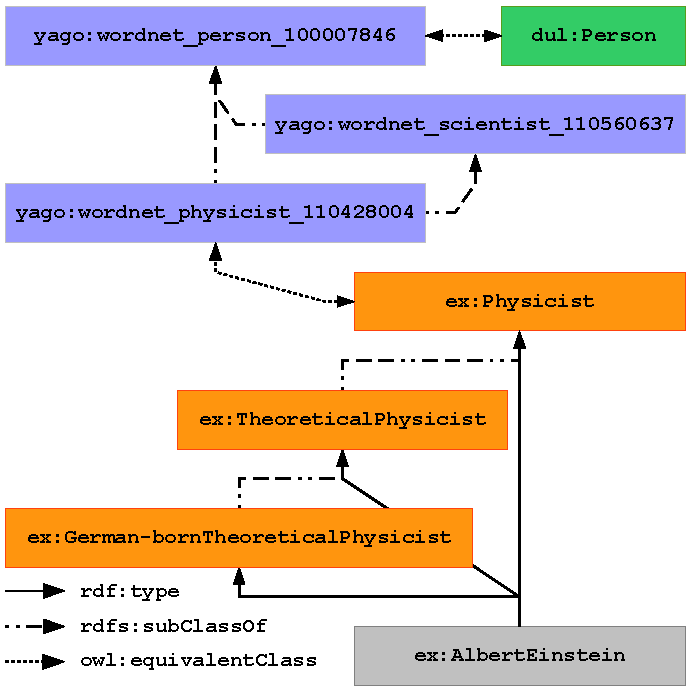
\includegraphics[scale=0.8]{chapter_three/unstructured_annotation/fig/localYAGOHierarchy.pdf}
\caption{Resulting type hierarchy that is created based on the YAGO ontology.}
\label{fig:localYAGOHierarchy}
\end{figure}

%\begin{table}
%\centering
%\begin{tabular}{@{}ll@{}}
%\toprule
%\textbf{Similarity} & \textbf{Formula/Explanation} \\ \midrule
%Dice-Coefficient Similarity &         \\
%Levenstein/Edit Similarity &         \\
%Euclidean Similarity &         \\ 
%Semantic Similarity &      Word2Vec   \\\bottomrule
%\end{tabular}
%\caption{Similarity measures of CETUS}
%\label{tab:stringsim}
%\end{table}

%CETUS' algorithms are easily extensible via its interfaces. 
%We will refine the set of string matching algorithms after the evaluation against the Open Knowledge Extraction task 2 corpora.

\section{Entity Type Linking using FOX}
\label{sec:typeLinking}

A second approach for a type extraction baseline is the usage of one of the various, existing entity typing tools.
For our second version CETUS$_{FOX}$, we are using FOX\footnote{\url{http://aksw.org/Projects/FOX.html}}, a named entity recognition and typing tool based on ensemble learning over 8 different tools.

CETUS$_{FOX}$ sends the given document to the FOX web-service for retrieving annotations.
If the entity inside the document is found and typed by FOX, the type is used to choose one of the four DOLCE+DnS Ultra Lite classes, see Table~\ref{tab:foxclassmatching}.
The chosen class is used as super class for the automatically created classes.
Unfortunately, FOX does not identify roles in its current version.

With respect to our running example, the FOX tool marks "Albert Einstein" as a person.
Thus, the created classes would be defined as subclasses of \texttt{dul:Person} as shown in Figure~\ref{fig:localFOXHierarchy}.

\begin{table}
\centering
\begin{tabular}{lp{5mm}l}
\toprule
 \multicolumn{1}{c}{FOX class} && DOLCE+DnS Ultra Lite class \\
\midrule
 \texttt{scmsann:PERSON} && \texttt{dul:Person} \\
 \texttt{scmsann:LOCATION} && \texttt{dul:Place} \\
 \texttt{scmsann:ORGANIZATION} && \texttt{dul:Organization} \\
 %\texttt{scmsann:OTHER} && \texttt{dul:Role} \\
\bottomrule
\end{tabular}
\caption{Mapping from FOX classes to DOLCE+DnS Ultra Lite classes.}
\label{tab:foxclassmatching}
\end{table}


\begin{figure}[htb!]
\centering
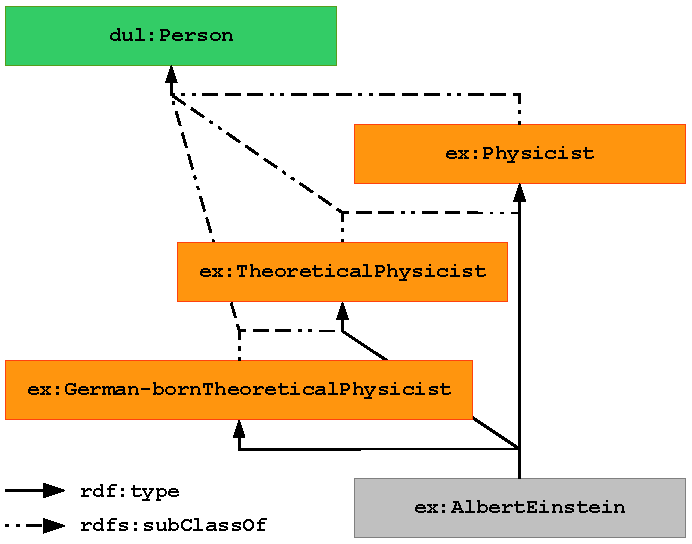
\includegraphics[scale=0.8]{chapter_three/unstructured_annotation/fig/localFOXHierarchy.pdf}
\caption{Resulting type hierarchy that is created based on the results of FOX.}
\label{fig:localFOXHierarchy}
\end{figure}

\section{Conclusion}
\label{cha321:sec:conclusion}

We presented CETUS---a pattern based type extraction that can be used as baseline for other approaches.
Both versions---CETUS$_{YAGO}$ and CETUS$_{FOX}$---have been explained in detail.
We showed how the first one uses a label matching for determining a super type for the automatically generated classes while the second is based on one of the various, existing entity typing tools.



%\usepackage{graphicx}
%\usepackage{subfigure}
%\usepackage{amsmath,amssymb}
%\usepackage[english]{babel}
%\usepackage[utf8]{inputenc}
%\usepackage[ruled,vlined]{algorithm2e}
%\usepackage{url}
%\usepackage{float}
%\usepackage{multirow} 
%\usepackage{booktabs}
%\usepackage[disable]{todonotes}
%\usepackage{todonotes}
%\usepackage{booktabs}
%\usepackage{mdframed}
%\usepackage{wrapfig}
%\usepackage{caption}
%\usepackage{tikz}
%\usepackage{verbatim}
%\usepackage{afterpage}
%\usepackage[active,tightpage]{preview}
%\PreviewEnvironment{tikzpicture}
%\setlength\PreviewBorder{5pt}%

%\usepackage{siunitx}%number formatting inside tables
\sisetup{
round-mode = places,
detect-family = true,
detect-inline-family = math,
detect-weight=true,
detect-inline-weight = math
}%

%\begin{document}


\chapter{Cross-Document Co-reference Resolution using Latent Features}


%\author{
%Axel-Cyrille Ngonga Ngomo$^{\diamondsuit}$ \and
%Michael R\"oder$^{\spadesuit\diamondsuit}$ \and 
%Ricardo Usbeck$^{\spadesuit\diamondsuit}$ 
%\institute{
%${\diamondsuit}$ University of Leipzig, Germany, 
%${\spadesuit}$ R\,\&\,D, Unister~GmbH, Leipzig, Germany, 
%\newline email: \{ngonga$|$usbeck\}@informatik.uni-leipzig.de
%}
%}

%\maketitle

%\newmdtheoremenv{ex}{Example}
\newcommand{\goodgap}{%
%\hspace{\subfigtopskip}%
%\hspace{\subfigbottomskip}
}
\todo[inline]{adjust goodgap}
%\begin{abstract}
Over the last years, entity detection approaches which combine named entity recognition and entity linking have been used to detect mentions of RDF resources from a given reference knowledge base in unstructured data. In this paper, we address the problem of assigning a single URI to named entities which stand for the same real-object across documents but are not yet available in the reference knowledge base. This task is known as cross-document co-reference resolution and has been addressed by manifold approaches in the past. We present a preliminary study of a novel take on the task based on the use of latent features derived from matrix factorizations combined with parameter-free graph clustering. 
%We study whether this approach achieves better results than the simple approaches used in most tools so far by measuring the accuracy of the clusters we detect on several benchmark datasets.
We study the influence of different parameters (window size, rank, hardening) on our approach by comparing the F-measures we achieve on the $\mbox{N}^3$ benchmark.
Our results suggest that using latent features leads to higher F-measures with an increase of up to 20.5\% on datasets of the $\mbox{N}^3$ collection.
%\end{abstract} 

%\todo[inline]{Full paper with a maximum of 12 pages including references
%Short paper with a maximum of 6 pages including references}

\section{Introduction}
%\todo[inline]{Removed: The abstact contains "deterministic matrix factorization algorithm". But is it still deterministic?}
%\todo[inline]{Axel}
The Document Web contains a large amount of information that is still not available on the Web of Data.
For example, open extraction frameworks for unstructured data have been shown to harvest a considerable amount of new triples pertaining to real-objects for which no URI is available~\cite{GER+13}.
While no URI has been assigned to the said real-world objects, facts pertaining to these objects can be distributed across manifold data sources.
Hence, simple URI generation approaches based on the labels of named entities can easily fail to generate the same URI when relying on two different labels that stand for the same real-world object.
For example, simple URI generation schemes based on strings would fail to generate the same URI when presented with the strings ``P. Diddy'' and ``Puff Daddy'' as labels for resources.
Moreover, they would generate the same URI for ``Golf'' across different documents even if the ``Golf'' stood for the sport in some documents and for the car in others.
In literature, detecting that two labels stand for the same real-object even across documents is referred to as \emph{cross-document co-reference resolution} (CDCR)~\cite{Andrews:2014fk,DBLP:journals/corr/BeheshtiVRBW13}.
While a large number of CDCR approaches have been developed in previous works (see Section~\ref{sec:sota}), none of the current approaches makes use of latent features to detect whether two labels stand for the same real-object. In previous work, latent features have yet been shown to be able to generate reliable representations of real-world objects~\cite{DBLP:conf/www/NickelTK12}.

In this paper, we address the aforementioned research gap by presenting the first CDCR approach based on latent features.
Our approach represents entity mentions as bags of words.
Each entity mention is then regarded as a vector in the space spanned by all words used to describe at least one entity mention.
In the subsequent step, we compute the latent features of the entity mentions.
The similarity of the latent representation of the entity mentions is then transformed into a similarity graph which is clustered by using BorderFlow~\cite{DBLP:conf/cicling/NgomoS09}, a parameter-free graph clustering approach.
All entity mentions which belong to the same cluster are regarded as mentions of the same real-world object and are assigned to the same URI.
Our approach is open-source and available at \url{http://github.com/AKSW/CoreferenceResolution}.

The rest of this paper is organized as follows:v
First, we give an overview of previous CDCR approaches.
Then, we present our approach in detail.
In Section~\ref{cha314:sec:evalval}, we evaluate our approach on the $\mbox{N}^3$ benchmark dataset~\cite{n3} and compare it with a baseline approach.
We conclude the paper and discuss future work in Section~\ref{cha314:sec:conclusion}.
%Most entity detection frameworks assume that they can map detected named entities to resources in knowledge bases and assign automatically generated URIs to named entities which stand for unknown resources.
%As they solve the URI generation problem locally, ...
%Over the last years, cross-document co-reference resolution approaches have been devised to help detect which

%Advantages: 
%* Automatic extraction of surface forms for known resources
%* Generation of rdfs:label for unknown resources
%* Improved disambiguation by using batch disambiguation instead of disambiguation for single 


\section{Related Work}
\label{sec:sota}
%\todo[inline]{Ricardo}
In the following section, we will provide an overview over recent approaches towards CDCR with a focus on their underlying techniques w.r.t. the semantic and syntactic features they exploit.
%Throughout the paper, we follow the nomenclature provided in~\cite{AGDISTIS_ECAI}.

Mayfield et al.'s~\cite{mayfield2009cross} CDCR approach comprises five stages: (1) intra-document processing, i.e., identification of mentions of entities, (2) entity pairs filtering, i.e., discarding of possible entity mappings to reduce computational costs, (3) calculating features of entities, (4) classification of entity matching by machine learning techniques and (5) clustering of entities to map each mention to the same equivalence class.
Unfortunately, the authors evaluated their approach in the ACE 2008 English named entity recognition task which is no longer available.
There, the approach achieved a value metric of 54.8~\cite{citeulike:5297302}.

Haghighi et al.~\cite{haghighi-klein:2010:NAACLHLT} present an unsupervised approach based upon a generative process which is capable to use modular syntactic and semantic features making use of latent information.
For every document, the generative process creates a number of entities mentioned in the text.
For every mention a noun phrase is created.
However, since the inference algorithm only uses these noun phrases, their approach lacks on taking a larger context into account.

Rahman et al.~\cite{Rahman+Ng:11a} introduce an approach which incorporates \emph{world knowledge} into two baseline CDCR algorithms.
Thereby, the authors use YAGO\footnote{\url{http://www.mpi-inf.mpg.de/departments/databases-and-information-systems/research/yago-naga/yago/}} and FrameNet\footnote{\url{https://framenet.icsi.berkeley.edu/fndrupal/}} as underlying knowledge bases.
Afterwards, they use a mention-entity pair classifier and a cluster-ranking model.
The results show an improvement over each baseline.
%\todo[inline]{find drawback}

Singh et al.~\cite{singh} present an approach consisting of (1) a large scale distributed inference mechanism based on Markov chain Monte Carlo methods and (2) they introduce sub-entity and super-entity variables representing clusters which are used to distribute or collect certain entities on a specific part of the machine cloud.
Furthermore, they evaluate their approach on a 1.5 million document comprising web crawl using anker tags to Wikipedia as gold standard.
%\todo[inline]{correct this paragraph, describe advantages over their approach}
Nevertheless, the authors approach misses the opportunity to consider latent features resulting in large computational costs w.r.t. the size of the resulting Markov chain.

Lee et al.~\cite{Lee:2012:JEE:2390948.2391006} present an approach not only capable of co-referencing entities but also events. 
Their idea is based upon linear regression which is used to merge clusters of entities. 
Furthermore, the authors featurize entities via semantic role labeling. 
Their approach is able to co-reference entities intra- and inter-document-wise.
Although the authors claim to be better than the state-of-the-art with respect to the CoNLL 2011 shared task~\cite{CoNLL} their published corpus is not available anymore.

In 2013, Beheshti et al.~\cite{DBLP:journals/corr/BeheshtiVRBW13} provide a systematic analysis of state-of-the-art CDCR systems.
The survey provides an in-depth structurization of the underlying methods and algorithms, which are widely used to solve CDCR problems on large scale. 
Furthermore, the authors highlight certain Big Data challenges, e.g., large amounts of pair-wise string similarity calculations and costly classification algorithms.

Normally, these approaches are based on a trained set of parameters for semantic and syntactic similarity algorithms.
Recently, Andrews et al.~\cite{Andrews:2014fk} describe an approach towards CDCR, here called entity clustering, that relies on learning parameters from test data without the need for training data. 
The generative process within assumes a mutation of semantic context and syntactic similarity while generating the documents with cross-referenced entities. 
Afterwards, the authors deploy a block Gibbs sampler to infer the clusters.
Unfortunately, this approach is only empirically evaluated.
%\todo[inline]{look for corpus: all corpora are available}

With respect to the clustering aspect of this paper, Schaeffer~\cite{schaeffer2007graph} provides an exhaustive overview of common graph-clustering algorithms and their use cases.

To the best of our knowledge, we present the first paper on CDCR based on latent features, matrix decomposition as well as graph-clustering.


\section{Approach}
In this section, we present our approach to CDCR in more detail. 
We introduce the notation necessary to understand the approach as required by each section.
Figure \ref{fig:SystemOverview} gives an overview of the five steps that underly our approach.
In a first step, a Matrix $M$ is generated containing the context of every entity mention.
After that, this matrix is decomposed into two smaller matrices $L$ and $R$ with $M \approx LR^{\top}$.
In parallel, a second matrix $S$ is created which contains the pairwise similarities of the labels of the entity mentions.
These matrices are used to generate a symmetric graph $G$ in which (1) every entity mention is a node and (2) two nodes are connected if their similarity is higher than a certain threshold.
$G$ is finally clustered.
Mentions that belong to the same cluster are considered to be mentions of the same entity.
Hence, they are all assigned the same URI.

\begin{figure}
\centering
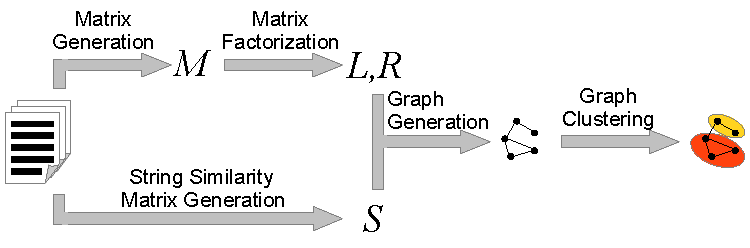
\includegraphics[width=0.9\textwidth]{chapter_three/unstructured_annotation/LD4IE_ISWC_CDCR/cdcr_SystemOverview.pdf}
\caption{The five steps of our approach.}
\label{fig:SystemOverview}
\end{figure}

%\todo[inline]{all: If somebody knows a program with which I can create a better picture than this, please let me know. Axel: Picture is fine}
%\todo[inline]{Micha: Refactor this section. Axel: Done}

\subsection{Matrix Generation}
%\todo[inline]{Micha}
The first step of our approach consists of generating a matrix which describes the context of every named entity mention inside the texts by means of a bag of words.
To this end, the given corpus is preprocessed by tokenizing the documents, removing stop words and indexing the remaining tokens.
In these tokenized documents, the context of a named entity mention is defined as the multiset of tokens inside a window with the size $\pm \sigma$ that is centered on the named entity's tokens.
The contexts are stored in a matrix $M$ containing a row for every named entity mention and a column for every indexed word.
The entries of the matrix are the counts of the words inside the entity mention's context.
As an example, let us consider the sentence 
\begin{ex}
\texttt{Yesterday, VW's CEO presented the new \underline{Golf} in Munich}.
\end{ex}
from which the stopwords \{\texttt{the}, \texttt{in}\} are removed.
For the window size $\sigma = 1$, we get the bag-of-word multiset \{\texttt{new} (1), \texttt{Munich} (1)\} as representation of ``Golf''.
Within the vector space spawned by (\texttt{presented}, \texttt{new}, \texttt{Munich}, \texttt{Germany}), this mention has the vector representation $(0, 1, 1, 0)$.
In the following, we will consider five entity mentions $g_1$, $g_2$, $g_3$, $g_4$ and $g_5$ labelled with the same word ``golf'' as example. 
These entity mentions will be assumed to be represented by the vectors 
$g_1 = (2,2,2,0)$, $g_2 = (1, 0, 0, 1)$, $g_3= (0,0,0,1)$, $g_4=(1, 0, 0, 0)$ and $g_5=(0, 1,1,0)$. 

\subsection{Matrix Factorization}
The matrix $M$ is now a matrix of dimensions $n \times m$ (denoted $M(n,m)$). 
The goal of a matrix factorization is to compute the matrices $L(n, \rho)$ and $R(m, \rho)$ such that $M \approx LR^{\top}$.
We call $\rho \in \mathbb{N} \backslash {0}$ the \emph{rank} of the factorization.
Several approaches have been used to factorize matrices.
Here, we loosely follow the tensor factorization approach presented in~\cite{DBLP:conf/www/NickelTK12}: Given two matrices $L$ and $R$ that are supposed to be the factors of $M$, the overall quadratic error of the approximation is the square Frobenius norm of $E = M - RL^{\top}$, i.e., $||E||_F^2 = ||M - RL^{\top}||_F^2$.
%We can express each entry of the squared Frobenius norm as follows:
%\begin{equation}
%e_{ij}^2 = \left(m_{ij} - \sum\limits_{k = 1}^r r_{ik}l_{jk}\right)^2.
%\end{equation}
%The error is minimal when the first partial derivative of $e_{ij}^2$ becomes 0.
%Thus, we need to minimize the values
%\begin{equation}
%\frac{\partial e_{ij}}{\partial r_{ik}} = -2 e_{ij}l_{jk} 
%\end{equation}
%and
%\begin{equation}
%\frac{\partial e_{ij}}{\partial l_{jk}} = -2 e_{ij}r_{ik}.
%\end{equation}
Previous works have shown that to prevent overfitting, the error function to minimize must be extended.
While several approaches have been suggested to this end, we adopt the error expression given by $||E||_F^2 - \frac{\lambda}{2}(||R||_F^2 + ||L||_F^2)$, where $\lambda \in [0, 1]$ controls how well $L$ and $R$ fit $M$. 
Thus, the error derivatives are as follows:
\begin{equation}
\frac{\partial e_{ij}}{\partial r_{ik}} = -2 e_{ij}l_{jk} + \lambda r_{ik}  
\end{equation}
 and 
\begin{equation}
\frac{\partial e_{ij}}{\partial l_{jk}} = -2 e_{ij}r_{ik} + \lambda l_{jk}.  
\end{equation}
We can now adopt a gradient descent approach to update the matrices $L$ and $R$ and reduce the error they lead to by overwriting each $l_{ik}$ resp $r_{jk}$ as follows:
\begin{equation}
l_{jk} \leftarrow l_{jk} - \alpha \frac{\partial e_{ij}}{\partial l_{jk}} = l_{jk} + \alpha \left(2 \sum\limits_{i=1}^n e_{ij}r_{ik} - \lambda l_{jk} \right)
\end{equation}
and
\begin{equation}
r_{ik} \leftarrow r_{ik} - \alpha \frac{\partial e_{ij}}{\partial r_{ik}} = r_{ik} + \alpha \left(2 \sum\limits_{j=1}^j e_{ij}l_{jk} - \lambda r_{ik} \right).
\end{equation}
We initialize $L$ and $R$ with random entries between 0 and $\max m_{ij}$.
%One problem that has remained unaddressed so far are the initialization of $L$ and $R$ as well as determining the correct settings for the parameters $r$, $\alpha$ and $\lambda$.
For our example, we get
\begin{equation}
M = \left(
\begin{matrix}
 2 & 2 & 2 & 0 \\
 1 & 0 & 0 & 1 \\
 0 & 0 & 0 & 1 \\
 1 & 0 & 0 & 0 \\
 0 & 1 & 1 & 0
\end{matrix} \right).
\end{equation}
For $\rho=2$, our approach computes
\begin{equation}
L = \left(
\begin{matrix}
  1.385 & 1.102 \\
 -0.006 & 0.501  \\
  0.079 & -0.051  \\
 -0.234 & 0.712 \\
  0.933 & -0.168
\end{matrix} \right)
\quad \text{and} \quad R = \left(
\begin{matrix}
 0.331 & 1.406 \\
 1.059 & 0.446 \\
 1.118 & 0.363 \\
 0.062 & 0.066
\end{matrix} \right).
\end{equation}
The intuition behind our approach is that $L$ is a better and compressed description of the entity mentions than $M$.
Hence, we now use $L$ in combination with a string similarity function to compute the similarity of entity mentions.

\subsection{String Similarity Matrix}
The string similarity matrix $S$ is an optional feature of our approach.
Each entry $s_{ij}$ of $S$ describes the similarity between the label of the $i$th and the $j$th entity in our input corpus.
Assuming a symmetric string similarity function such as the 3-gram similarity (which we use in our experiments), 
we also get a symmetric string similarity matrix $S$.
%Compute string similarity matrix $S$ using $n$-gram similarity with $n=3$.
We assume $s_{ij} = 1$ if no string similarity is specified.
$s_{ij} = 1$ also holds for our example, as all mentions are labelled with ``golf''.

\subsection{Graph Generation}
The aim of the graph generation is to generate a similarity graph $G = (V, E, w)$ that will allow detecting mentions of the same real-world object through clustering.
The set of vertices of $V$ is the set of entity mentions in our corpus.
We define the weight function $w: V \times V \rightarrow [0, 1]$ as $w(v_i, v_j) = s_{ij} \times \frac{l_{(i,\cdot)} \cdot l_{(j,\cdot)}}{||l_{(i,\cdot)}|| \times ||l_{(j,\cdot)}||}$, where $l_{(i,\cdot)}$ is the $i$th row-vector of $L$ and stands for the latent description of the $i$th entity mention in the corpus.
Given that many graph clustering approaches are polynomial in the number of edges, we can control $|E|$ by only setting an edge between $v_i$ and $v_j$ if $w(v_i, v_j) \geq \theta \in [0, 1]$.
%Remove edges with $g_{ij} \le \theta$ (=threshold)
For $\theta = 0.3$ and $\rho=2$ we end up with the graph displayed in Figure~\ref{fig:latent}. 
As comparison, Figure~\ref{fig:original} shows the graph obtained with by setting $L = M$, i.e., generating $G$ without using latent features.

\begin{figure}
\centering
\usetikzlibrary{arrows}

\begin{tikzpicture}[auto,node distance=2cm,
  thick,main node/.style={circle,fill=blue!20,draw,font=\sffamily\bfseries}]

  \node[main node] (1) {$g_1$};
  \node[main node] (2) [below left of=1] {$g_2$};
  \node[main node] (3) [above left of=1] {$g_3$};
  \node[main node] (4) [above right of=1] {$g_4$};
  \node[main node] (5) [below right of=1] {$g_5$};

  \path[every node/.style={font=\sffamily\small}]
    (1) edge node [left] {0.61} (2)
        edge node [left] {0.31} (3)
        edge node [left] {0.34} (4)
        edge node [left] {0.61} (5)
    (3) edge node [below] {0.95} (4)
    (2) edge node [above] {0.92} (5);    
\end{tikzpicture}
\caption{Graph generated using $\rho=2$}
\label{fig:latent}
\end{figure}

\begin{figure}
\centering
\usetikzlibrary{arrows}
\begin{tikzpicture}[auto,node distance=2cm,
  thick,main node/.style={circle,fill=blue!20,draw,font=\sffamily\bfseries}]

  \node[main node] (1) {$g_1$};
  \node[main node] (2) [below left of=1] {$g_2$};
  \node[main node] (3) [above left of=1] {$g_3$};
  \node[main node] (4) [below right of=1] {$g_4$};
  \node[main node] (5) [above right of=1] {$g_5$};

  \path[every node/.style={font=\sffamily\small}]
    (1) edge node [left] {0.41} (2)
        edge node [left] {0.58} (3)
        edge node [left] {0.82} (5)
    (2) edge node [left] {0.71} (3)
    (2) edge node [above] {0.71} (4);    
\end{tikzpicture}
\caption{Graph generated using $M$ instead of $L$}
\label{fig:original}
\end{figure}

\subsection{Graph Clustering}
%\todo[inline]{Axel}
We now cluster the graph $G$ to detect mentions that stand for the same real-world object.
Our approach can rely on any graph clustering approach.
In our current implementation, we rely on the BorderFlow algorithm~\cite{DBLP:conf/cicling/NgomoS09} because it is parameter-free.
BorderFlow regards any set $C \subseteq V$ as having a \emph{border} $b(C) = \{v \in C: \exists u \in V \backslash C \mbox{ with } (v, u) \in E\}$.
The \emph{flow} $\Omega(C_1, C_2)$ between two sets $C_1 \subseteq V$ and  $C_2 \subseteq V$ is defined as $\Omega(C_1, C_2) = \sum\limits_{v \in C_1, u \in C_2} w(v, u)$.
Based on these definitions, BorderFlow implements a local graph clustering paradigm by mapping each node $v \in V$ to the set of nodes $C \subseteq V$ that is such that $v \in C$ and $C$ is a node-maximal set w.r.t. the function 
\begin{equation}
bf(C) = \frac{\Omega(b(C), C)}{\Omega(b(C), V \backslash C)}.
\end{equation}
While finding the optimal $C$ for each $v$ can be very time-consuming, the heuristic presented in~\cite{DBLP:bibsonomy_NGO10b} allows determining an approximation of $C$ in an efficient manner.
We employ this heuristic herein.

Now, the result of BorderFlow is not a partitioning of the graph.
Rather, clusters may overlap.
We thus employ a \emph{hardening} approach to generate a partitioning of the input graph.
To this end, each node $v\in V$ which belongs to two different clusters $C_1$ and $C_2$ is assigned to $C_1$ iff
\begin{equation}
bf(C_1 \cup \{v\}) + bf(C_2 \backslash \{v\}) \geq bf(C_2 \cup \{v\}) + bf(C_1 \backslash \{v\}).
\end{equation}
In all other cases, $v$ is assigned to $C_2$.
We call this form of hardening \emph{flow maximization}.
Other forms of hardening can be conceived of, e.g., minimizing the number of unions operations that need to be carried out to achieve a partitioning of the graph (\emph{set-based}).

For our example, we get the clusters $\{g_1, g_5\}$ and $\{g_2, g_3, g_4\}$ for $\rho=2$ when using BorderFlow with any partitioning approach.
If we replace $L$ with $M$, we get the clusters  $\{g_1\}$, $\{g_2, g_4\}$ and $\{g_3, g_5\}$.
This result on toy data already suggests that matrix factorization leads to results that differ from those gathered when using raw data.
In the subsequent section, we show empirically that using $L$ to generate $G$ leads to more accurate results than using $M$ to generate $G$.

\section{Evaluation}

\label{cha314:sec:evalval}

\subsection{Experimental Setup}

\subsubsection{Goals}
The goal of our experiments was two-fold. First, we wanted to measure the effect of the different parameters on our approach.
Moreover, we wanted to know whether the factorization outperforms a comparable baseline.
To achieve the first goal of our experiments, we conducted experiments where we varied the rank $\rho$ as well as the window size $\sigma$ while keeping all other parameters fixed.
We addressed the second goal by creating a baseline as follows: We ran our pipeline as described in the sections above with the sole difference that (1) we did not carry out a factorization and (2) we use $M$ instead of $L$ as input for the graph clustering. All other steps (matrix generation, graph generation, graph clustering) remained unchanged.
The similarity threshold for the graph generation is set to $\theta=0.1$ for all our experiments.

\subsubsection{Datasets}
We use the three corpora of the $\mbox{N}^3$ collection~\cite{n3} in our experiments.
%\todo[inline]{Actually here could be an error, which leads to very high f-measure}
%Each corpus was annotated manually, i.e., each entity mention was mapped to an URI from DBpedia~\cite{lehmann2014dbpedia} or a URI from the \url{http://aksw.org/} namespace if no corresponding resource could be found in DBpedia.
%
\begin{itemize}
\item The \textbf{News-100} corpus comprises 100 German news articles from \url{news.de}.
Each of these articles contains the German word ``Golf''---a homonym that has three different meanings inside these documents.
The word could mean (a) a gulf, e.g., the Mexican gulf, (b) the ball sport or (c) a compact car of the German manufacturer Volkswagen.
This is clearly the most difficult dataset, as many resources share exactly the same name but have different meanings. 
\item The \textbf{Reuters-128} corpus contains 128 English economy news articles from the Reuters news agency.
The documents in this dataset are smaller than the ones from the News-100 corpus providing a shallow context.
\item The third corpus, \textbf{RSS-500}, contains 500 documents each with only one sentence.
The sentences were randomly chosen from a larger amount of RSS news feeds, as described in~\cite{GER+13}.
Every sentence contains exactly two named entities.
\end{itemize}
Table~\ref{tab:corpusStats} provides further detailed information about the corpora.
On average, each named entity occurs nearly 5 times in the News-100 corpus.
Within the Reuters-128 corpus nearly two mentions per named entity exist on average while in the RSS-500 corpus only every tenth entity is mentioned more than once.

%\todo[inline]{Micha: describe N${}^{3}$}

\begin{table}[thb]
    \caption{Features of the corpora}
    \begin{tabular}{lp{0.7cm}rp{0.3cm}p{0.7cm}rp{0.2cm}p{0.6cm}rp{0.3cm}}
    \toprule
     & \multicolumn{3}{c}{\textbf{News-100}} & \multicolumn{3}{c}{\textbf{Reuters-128}} & \multicolumn{3}{c}{\textbf{RSS-500}} \\
    \midrule
    Documents && 100 &&& 128 &&& 500 &\\
	Tokens && 48199 &&& 33413 &&& 31640 &\\
	Entities && 362 &&& 444 &&& 849 &\\
    Mentions && 1655 &&& 880 &&& 1000 &\\
	\bottomrule
	\end{tabular}
	\centering
	\label{tab:corpusStats}
\end{table}

\subsection{Results}

\subsubsection{Influence of rank}
In our first series of experiments, we fixed the window size to 4 and measured the influence of the rank $\rho$ on the precision, recall and F-measure. 
The left side of Figure~\ref{fig:results} shows the results of our experiments on the three datasets.
Most importantly, our results show that we outperform the baseline in most settings.
We achieve the best increase of performance on the RSS-500 corpus, where we achieve a 20.5\% increase in F-measure over the baseline.
This result suggest that our approach does not tend to overgeneralize through the compression on information that is carried out during the factorization.
Instead, our results suggest that we get rid of a significant amount of noise while factorizing.
Our results on the other two datasets show that we also achieve a better F-measure (increases of 18.2\% on Reuters-128 and 6.3\% on News-100, see Table~\ref{tab:improvements}). 
An analysis of the results reveals that this increase is mostly due to the significant increase in precision that we achieve in most settings.
On the other hand, our recall is rarely ever worse than that of the baseline.
This suggests that BorderFlow tends to generate smaller clusters with factorization than when the baseline approach is used.
We measure the statistical significance of our results using a Wilcoxon signed rank-test with 95\% confidence.
Our results are significant in all cases.%\todo[inline]{Check this}

\subsubsection{Influence of window size}
In this experiment, we set the rank to 100 for all experiments and measured the effect of the window size on the overall F-measure of our approach.
The right half of Figure~\ref{fig:results} shows the results of this series of experiments on the three datasets.
Overall, our results suggest that for this rank, the window size does not have a major influence on the F-measure. 
This also seems to hold for other ranks.
Interestingly, a small window size seems to lead to good results in most cases when we use the factorization. While we assume that this might be due to the factorization being able to convert the two words within the window to their latent features    
This result indicates that small window sizes suffice for our approach to achieve better F-measures than the baseline on the CDCR problem.
This might mean that a small set of words is already sufficient to disambiguate resources across different documents.

\begin{figure}[t!]
\centering
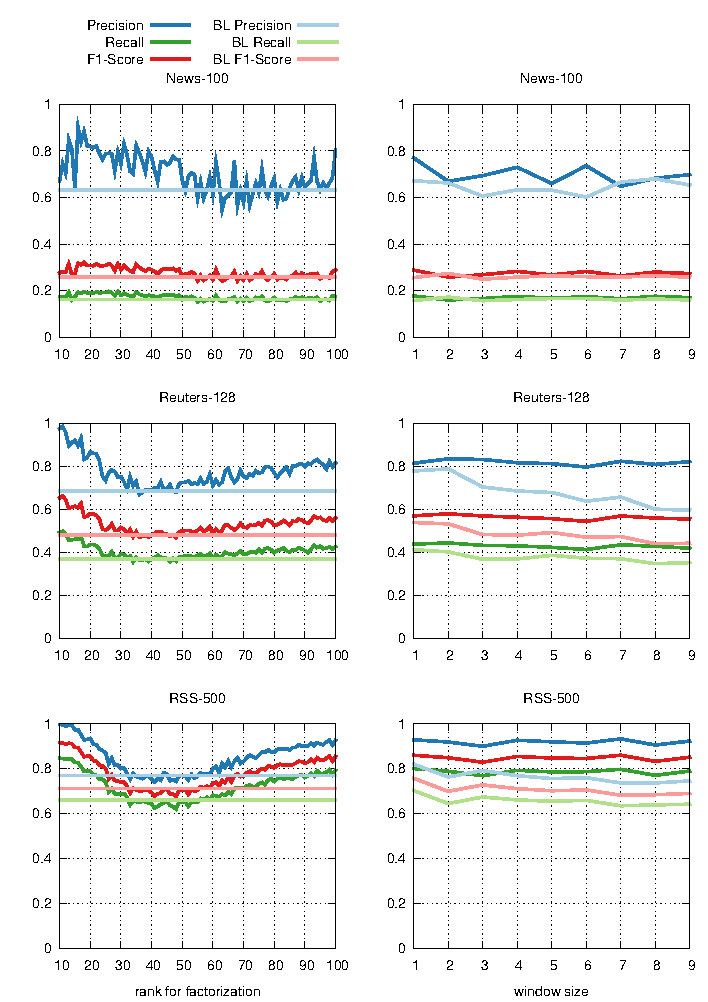
\includegraphics[width = \textwidth]{chapter_three/unstructured_annotation/LD4IE_ISWC_CDCR/cdcr_results_Flow.pdf}
\caption{Precision, recall and F1-score of our approach with different ranks (left) and different window sizes (right) compared to the baseline (BL). The diagrams show the results for the flow maximization hardening.}
\label{fig:results}
\end{figure}
\afterpage{\clearpage}

\subsection{Effect of hardening}
In all results presented above, we used a hardening based on the borderflow ratio.
We also implemented the set-based hardening mentioned above and compared the results we achieve with this hardening.
Overall, our results suggest that the borderflow-maximization approach that we used for hardening generates the best results both for the baseline and our approach. 
Moreover, we outperform the baseline independently from the hardening used.

\begin{table}[htb]
    \caption{Best improvements in F-measure of our approach (OA) over the baseline (BL)}
    \begin{tabular}{lp{1cm}p{0.25cm}rp{1cm}p{0.25cm}rp{1cm}p{0.25cm}rp{1cm}p{0.25cm}r}
    \toprule
     && \multicolumn{5}{c}{\textbf{Flow Maximization}} && \multicolumn{5}{c}{\textbf{Set-Based}} \\
     && \multicolumn{2}{c}{BL} && \multicolumn{2}{c}{OA} && \multicolumn{2}{c}{BL} && \multicolumn{2}{c}{OA} \\
    \midrule
    News-100        &&& 25.86  &&& \textbf{32.21} &&& 23.87  &&& \textbf{28.81} \\
	Reuters-128     &&& 47.89  &&& \textbf{66.16} &&& 47.00  &&& \textbf{56.65} \\
	RSS-500         &&& 71.11  &&& \textbf{91.62} &&& 69.57  &&& \textbf{85.71} \\
	\bottomrule
	\end{tabular}
	\centering
	\label{tab:improvements}
\end{table}

%\subsection{Scalability}\todo[inline]{Please fill gaps}
%One last question that we addressed is the scalability of our approach.
%We ran our experiments on a Debian machine (Intel Xeon 3.10GHz, 8GB RAM).
%On average, the baseline experiments ran 22.7s for News-100, ??? for Reuters-128 and ??? for RSS-500.
%In contrast, the experiments with factorization ran ??? for News-100, ??? for Reuters-128 and ??? for RSS-500.
%These results suggest that our approach scales when and does not produce a significant overhead in runtime while generating significantly better results.

\subsubsection{Discussion}
Overall, our initial results suggest that we indeed outperform the proposed baseline by using matrix factorization (see Table~\ref{tab:improvements}).
Still, many questions do remain open.
The most important question that we did not address is when should a high rank be used?
First, in our experiments, $\rho=10$ was sufficient across all datasets to outperform the baseline. 
To the best of our knowledge, finding the optimal rank for a factorization problem is an open question.
Nevertheless, we think that the answer to this question lies in the amount of information contained in the corpus.
The higher the information density of a corpus, the higher the rank required to characterize entity adequately.
A second question that remains unanswered is whether we can improve the results of the factorization by considering known resources in the dataset.
We will address this question in future work by disambiguating using a combination of textual information and Linked Data.
%\todo[inline]{Micha: Refactor the current figure. It doesn't look really nice.}

%\subsubsection{Runtime}
%We also measured the runtime of our approach across all experiments. Our results suggest that our approach can actually lead to significantly smaller runtimes. However, the settings in which we achieve the best runtimes correspond to settings in which the overall runtime of our approach is comparable to that of the baseline. This is obviously a satisfactory results as it means that we can achieve better F-measure without requiring significantly higher processing times.

\section{Conclusion}
\label{cha314:sec:conclusion}
In this paper, we presented a CDCR approach based on latent features.
We showed that our approach can outperform our baseline by more than 10\% F-measure.
%Moreover, we showed that our approach scales well and can thus be used on large datasets.
We will use our approach to complement the entity linking framework~\cite{agdistis_iswc} when it is used in batch mode, i.e., over a document corpus at once.
Moreover, we will develop means to detect an appropriate rank for factorization.
To this end, we plan to use the derivative of the mean squared error $||M - LR^{\top}||^2_F$.
Finally, we will develop a deterministic approach to initialize $L$ and $R$. 
Preliminary results on random matrices show that we can already reduce the initial value of $||E||^2_F$ by more approximately 40\%, leading to a significantly faster convergence of the factorization.



%\end{document}


\begin{comment}
\begin{table}[htb]
    \caption{Best improvements of our approach over the baseline}
    \begin{tabular}{lp{0.5cm}cp{0.5cm}cp{0.5cm}c}
    \toprule
     && \multicolumn{1}{c}{\textbf{Rank}} && \multicolumn{1}{c}{\textbf{Baseline (F1)}} && \multicolumn{1}{c}{\textbf{Our approach (F1)}} \\
    \midrule
    News-100        && 11   && 56.78  && 62.99 \\
	Reuters-128     && 91   && 68.23  && 71.63 \\
	RSS-500         && 97   && 79.31  && 88.40 \\
	\bottomrule
	\end{tabular}
	\centering
	\label{tab:improvements}
\end{table}
\end{comment}

\begin{comment}
\subsection{Initialization of $L$ and $R$}
In most approaches, the matrices $L$ and $R$ are initialized by using random values.
While this approach still leads to converging results in practical applications, it is unsatisfactory as the results of the factorization may be different across different initializations.
We address the initialization problem by using a correlation-based approach.
The intuition behind our approach is that the latent features describe a space whose basic vectors stand for weakly correlated dimensions. 
We can thus initialize the matrices $L$ (and analogously the matrix $R$) by detecting the rows (resp. columns) that display the smallest correlation to other rows and using those as our initialization for $L$.
We go about implementing this intuition as follows: Let 
\begin{equation}
B = M \times M^\top \mbox{ and } A = \frac{B}{\max\limits_{i, j} b_{ij}}.
\end{equation}
The matrix $A$ encompasses how correlated the rows in $M$ are.
We assign each row $a_{i}$ a weight $w_i = \sum_{j=1}{n} a_{ij}$.
The weight $w_i$ tells us how correlated $a_i$ is to $a_1 \ldots a_n$.
We now sort the rows according to their weights in ascending order and select the r rows with the smallest weight.
These rows are then used to initialize $L$, ergo $l_1 = a_k$ with $\forall i \neq k, w_i \geq w_k$.  

The matrix $R$ can be initialized analogously by setting 
\begin{equation}
B = M^\top \times M \mbox{ and } A = \frac{B}{\max\limits_{i, j} b_{ij}}.
\end{equation}
\todo{Add example}

\begin{itemize}
\item use FOX to do NER over several documents \todo{No need for FOX in the experiments. Simply use the benchmarks directly.} 
\todo{Now it is implemented and getting back to the original work would be cumbersome.} 
\item describe an entity by its neighbors, i.e., window size and latent features
\item use cosine similarity as a baseline
\item cluster those entities across documents using Axels framework
\item named entities are the same resources if they end up in the same cluster...\todo[inline]{RU: I fear the noise hear when number of clusters is too low}
\item formulate good URIs for them, see http://www.w3.org/TR/cooluris/

\end{itemize}

LR^T = 

  5,103 1,896 -0,712 1,555
  3,412 1,274 -0,450 1,085
  1,540 1,040  1,780 3,949
  1,169 0,799  1,394 3,073
 -0,438 0,543  3,076 5,125
\end{comment}



\documentclass{acm_proc_article-sp}

\usepackage{graphicx}
\usepackage{pifont}
\usepackage{amsmath,amssymb}
\usepackage[english]{babel}
\usepackage[utf8]{inputenc}
\usepackage[ruled,vlined]{algorithm2e}
\usepackage{hyperref}
\usepackage{float} 
\usepackage{multirow} 
\usepackage{booktabs}
%\usepackage[disable]{todonotes}
\usepackage{todonotes}
\usepackage{mdframed}
\usepackage{wrapfig}
\usepackage{booktabs}
\usepackage{tabulary}
\usepackage{comment}
\usepackage{tikz}
\usepackage{xspace}


\newcommand{\haken}{{\ding{51}}}
\newcommand*\rot{\rotatebox{87}}
\newcommand{{\overalldatasets}}{11\xspace}
%ACE2004
%AQUAINT
%MSNBC
%IITB
%Meij
%AIDA/CoNLL
%N3 - reuters-128
%N3 - rss-500
%KORE50
%Spotlight Corpus
%Microposts
\newcommand{{\numberOfadditionalDatasets}}{6\xspace}
%N3 - reuters-128,N3 - rss-500,KORE50,Spotlight Corpus, Microposts, Ace2004
\newcommand{{\overallGERBILannotators}}{9\xspace}
%without NIF-based Annotator
%Wikipedia Miner
%Spotlight
%TagMe 2
%KEA
%WAT
%AGDISTIS
%Babelfy
%NERD-ML
%Dexter
\newcommand{{\numberOfBATAnnotators}}{5\xspace}
%AIDA , Illionois Wikifier + Spotlight, Miner, TagMe
\newcommand{{\numberOfadditionalAnnotators}}{6\xspace}
%KEA, WAT, AGDISTIS, Babelfy, NERD-ML, Dexter
\newcommand{{\overallNrOfMatchingTypes}}{3\xspace}
%Strong Annotation Matching, Weak Annotation Matching, Strong Entity Matching


\begin{document}

\title{GERBIL -- General Entity Annotator Benchmarking Framework}
\numberofauthors{21}
\author{
\alignauthor Ricardo Usbeck\thanks{Further co-authors can be found at the end of the article.}\\
       \affaddr{Leipzig University, IFI/AKSW}\\
       \affaddr{Unister GmbH, Leipzig}\\
       \email{usbeck@informatik.\\uni-leipzig.de}
\alignauthor Michael R\"oder$^{*}$\\
       \affaddr{Leipzig University, IFI/AKSW}\\
       \affaddr{Unister GmbH, Leipzig}\\
       \email{roeder@informatik.\\uni-leipzig.de}
\alignauthor Axel-Cyrille Ngonga Ngomo$^{*}$\\
       \affaddr{Leipzig University, IFI/AKSW}\\
       \affaddr{Leipzig (Germany)}\\
       \email{ngonga@informatik.uni-leipzig.de}
}
\additionalauthors{
%%%% ordered alphabetically
Ciro Baron (Leipzig University, Germany)\\
Andreas Both (R\&D, Unister GmbH, Germany)\\
Martin Brümmer (Leipzig University, Germany)\\
Diego Ceccarelli (University of Pisa, Italy)\\
Marco Cornolti (University of Pisa, Italy)\\
Didier Cherix (R\&D, Unister GmbH, Germany)\\
Bernd Eickmann (R\&D, Unister GmbH, Germany)\\
Paolo Ferragina (University of Pisa, Italy)\\
Christiane Lemke (R\&D, Unister GmbH, Germany)\\
Andrea Moro (Sapienza University of Rome, Italy)\\
Roberto Navigli (Sapienza University of Rome, Italy)\\
Francesco Piccinno (University of Pisa, Italy)\\
Giuseppe Rizzo (EURECOM, France)\\
Harald Sack (HPI Potsdam, Germany)\\
Ren\'{e} Speck (Institute for Applied Informatics, Germany)\\
Rapha\"el Troncy (EURECOM, France)\\
J\"org Waitelonis (HPI Potsdam, Germany)\\
Lars Wesemann (R\&D, Unister GmbH, Germany)\\
%%%% contributed already
%Pablo Mendes (Yahoo, USA)\\
%Andreas Blumauer (Semantic Web Company, Austria)\\
}

\maketitle
% Important sources: http://mucmd.org/slides/mucmd2012-gil.pdf
% 
\begin{abstract}
The need to bridge between the unstructured data on the Document Web and the structured data on the Web of Data has led to the development of a considerable number of annotation tools. However, these tools are currently still hard to compare since the published evaluation results are calculated on diverse datasets and evaluated based on different measures. 
We present GERBIL, an evaluation framework for semantic entity annotation. The rationale behind our framework is to provide developers, end users and researchers with easy-to-use interfaces that allow for the agile, fine-grained and uniform evaluation of annotation tools on multiple datasets. By these means, we aim to ensure that both tool developers and end users can derive meaningful insights pertaining to the extension, integration and use of annotation applications. In particular, GERBIL provides comparable results to tool developers so as to allow them to easily discover the strengths and weaknesses of their implementations with respect to the state of the art. With the permanent experiment URIs provided by our framework, we ensure the reproducibility and archiving of evaluation results. Moreover, the framework generates data in machine-processable format, allowing for the efficient querying and post-processing of evaluation results. Finally, the tool diagnostics provided by GERBIL allows deriving insights pertaining to the areas in which tools should be further refined, thus allowing developers to create an informed agenda for extensions and end users to detect the right tools for their purposes. GERBIL aims to become a focal point for the state of the art, driving the research agenda of the community by presenting comparable objective evaluation results.
%\todo[inline]{AnBo: I think the aim is threefold: users, developers, academics. Additionally, I would like to add: GERBIL will become a focal point for the state of the art, driving the research agenda of the community by presenting comparable objective evaluation results. Axel: Done},
\end{abstract}

\section{Introduction}
%\todo[inline]{RU: I am missing a bit the extension of BAT in terms of datasets, annotators and experiment types}
The implementation of the original vision behind the Semantic Web demands the development of approaches and frameworks for the seamless extraction of structured data from text. 
While manifold annotation tools have been developed over the last years to address (some of) the subtasks related to the extraction of structured data from unstructured data \cite{TagMe2,AIDA,spotlight,milne2008learning,babelfy,piccinno2014tagme,rizzo2014,Steinmetz2013,AGDISTIS_ISWC}, the provision of comparable results for these tools remains a tedious problem. The issue of  comparability of results is not to be regarded as being intrinsic to the annotation task. Indeed, it is now well established that scientists spend between 60 and 80\% of their time preparing data for experiments \cite{GIL2014,jermyn1999preparing,peng2011reproducible}. Data preparation being such a tedious problem in the annotation domain is mostly due to the different formats of the gold standards as well as the different data representations across reference datasets.
%\todo[inline]{AnBo: --change-- different formatting of the textual data in reference datasets --to-- different data representations in reference datasets. Axel:Done}
These restrictions have led to authors evaluating their approaches on datasets (1) that are available to them and (2) for which writing a parser as well as of an evaluation tool can be carried out with reasonable effort.
%\todo[inline]{AnBo: easy sounds like an affront, suggestion: is easy --to-- can be implemented within reasonable effort. Axel: Done.} 
In addition, a large number of quality measures have been developed and used actively across the annotation research community to evaluate the same task, leading to the results across publications on the same topics not being easily comparable. For example, while some authors publish macro-F-measures and simply call them F-measures, others publish micro-F-measures for the same purpose, leading to significant discrepancies across the scores. The same holds for the evaluation of how well entities match. Indeed, partial matches and complete matches have been used in previous evaluations of annotation tools \cite{Cornolti,fox}. This heterogeneous landscape of tools, datasets and measures leads to a poor repeatability of experiments, which makes the evaluation of the real performance of novel approaches against the state of the art rather difficult.

The insights above have led to a movement towards the creation of frameworks to ease the evaluation of solutions that address the same annotation problem~\cite{ERD2014,Cornolti}. In this paper, we present GERBIL -- a general entity annotator benchmark --, a community-driven effort to enable the continuous evaluation of annotation tools. GERBIL is an open-source and extensible framework that allows evaluating tools against (currently) \overallGERBILannotators different annotators on \overalldatasets different datasets within 6 different experiment types. 
%At this point in time, GERBIL integrates . Moreover, \overallNrOfMatchingTypes matching types are provided. 
By integrating such a large number of datasets, experiment types and frameworks, GERBIL allows users to evaluate their tools against other semantic entity annotation systems (short: entity annotation systems) by using exactly the same setting, leading to fair comparisons based on exactly the same measures. 
While the evaluation core of GERBIL is based on the BAT-framework \cite{Cornolti}, our approach goes beyond the state of the art in several respects:
\begin{itemize}
\item GERBIL provides \emph{persistent URLs} for experimental settings. Hence, by using GERBIL for experiments, tool developers can ensure that the settings for their experiments (measures, datasets, versions of the reference frameworks, etc.) can be reconstructed in a  unique manner in future works. 
\item Through experiment URLs, GERBIL also addresses the problem of \emph{archiving} experimental results and allows end users to gather all pieces of information required to choose annotation frameworks for practical applications.
\item GERBIL aims to be a \emph{central repository for annotation results} without being a central point of failure: While we make experiment URLs available, we also provide users directly with their results to ensure that they use them locally without having to rely on GERBIL.
\item The results of GERBIL are published in a \emph{machine-readable format}. In particular, our use of DataID~\cite{dataID} and DataCube~\cite{datacube} to denote tools and datasets ensures that results can be easily combined and queried (for example to study the evolution of the performance of frameworks) while the exact configuration of the experiments remains uniquely reconstructable. By these means, we also tackle the problem of \emph{reproducibility}. 
\item Through the provision of results on different datasets of different types and the provision of results on a simple user interface, GERBIL also provides means to quickly gain an overview of the current performance of annotation tools, thus providing (1) developers with insights pertaining to the type of data on which their accuracy needs improvement and (2) end users with insights allowing them to choose the right tool for the tasks at hand.
\item With GERBIL we introduce the notion of knowledge base-agnostic benchmarking of entity annotation systems through generalized experiment types. By these means, we allow benchmarking tools against reference datasets from any domain grounded in any reference knowledge base. 
\end{itemize}
%\todo[inline]{@Axel: read last item}
%\todo[inline]{formulate item about generelization introduced ie knowledge base agnostic experiment types.}

%Reproducibility of research is a widely acknowledged issue in various domains of science. Without the ability of easily replicating results, the scientific community cannot judge claims and hypotheses of scientists or build supportive or rejective evidence \cite{peng2011reproducible}. In many domains of computational science however, replication and verification of submitted or published results can be a very painful process consuming a lot of time and resources. 

%The recent uptake of semantic technologies leads to a growing number of information extraction algorithms. 
%In particular, named entity recognition (NER) and disambiguation/linking (NED) approaches to Wikipedia or DBpedia~\cite{dbpedia-swj}, respectively, are a key point of semantic research.
%Unfortunately, to the best knowledge of the authors, there is no comprehensive and up-to-date overview of NER or NED approaches yet, despite the fact that there are a large amount of open source, webservice-based and freely available projects.
%\todo[inline]{Giuseppe: comprehensive is a bit misleading here and it might be seen as controversial (for instance in our LREC'14 paper we have provided experiments and discussions for NER mainly and introduced NEL. Also Cornolti et al. has proposed an overview of the NEL task.). It's better to list what are the things not yet addressed and the contributions of the paper, perhaps linking this part with the points reported below.}
%Additionally, only a small number of scientific articles publish either experimental data, software or comprehensive configuration settings independent of the domain.
%\todo[inline]{I think the "independent of the domain" could be too strong, as replication is more widely adopted in fields like medical research and physics (christiane)}


%\todo[inline]{deadline: Nov 5, put numbers here}
%In this paper, we introduce GERBIL -- a general entity annotator benchmark -- which is a web-based platform for comparing ZZZZ different NER and NED approaches on a large amount of freely available datasets with XXX different metrics and via YYY different experiment types to reproduce a large number of results at a time.

%To achieve this, we reused parts of the benchmarking framework introduced 2013 by Cornolti et al.\cite{Cornolti}, dubbed BAT-Framework.

%\todo[inline]{check contributions table on the 5th whether we really do it}

To ensure that the GERBIL framework is useful to both end users and tool developers, its architecture and interface were designed with the following principles in mind:

\begin{itemize}
\item \textbf{Easy integration of annotators}: We provide a wrapping interface that allows annotators to be evaluated via their REST interface. In particular, we integrated \numberOfadditionalAnnotators additional annotators not evaluated against each other in previous works (e.g., \cite{Cornolti}).  
\item \textbf{Easy integration of datasets}: We also provide means to gather datasets for evaluation directly from data services such as DataHub.\footnote{\url{http://datahub.io}} In particular, we added \numberOfadditionalDatasets new datasets to GERBIL.
\item \textbf{Easy addition of new measures}: The evaluation measures used by GERBIL are implemented as interfaces. Thus, the framework can be easily extended with novel measures devised by the annotation community.
\item \textbf{Extensibility}: GERBIL is provided as an open-source platform\footnote{Available at \url{http://gerbil.aksw.org}.} that can be extended by members of the community both to new tasks and different purposes.
\item \textbf{Diagnostics}: The interface of the tool was designed to provide developers with means to easily detect aspects in which their tool(s) need(s) to be improved. 
\item \textbf{Portability of results}: We generate human- and machine-readable results to ensure maximum usefulness and portability of the results generated by our framework. 
%\item 
%\item we generated a generic interface as adaptor for external datasets to enhance interoperability with next generation annotators and to allow for testing with closed source text corpora,
%\item we added XXXXXX new and publicly available datasets to the framework,
%\item GERBIL consists of a generic adaptor for external closed source algorithms,
%\item an easy-to-use web frontend for fast examination of annotator quality and
%\item provides citations of calculated results via unique URIs which will be stable over long periods of time,
%\item results are available as RDF, especially dataid and cube voc.
\end{itemize}

%It is our vision that GERBIL should become a central point for the IR and Semantic Web community to facilitate a common knowledge about named entity disambiguation and linking quality. 
%Each and every experiment should be comparable and reproducible with up-to-date webservices. 
%\todo[inline]{@MichaelRoeder: do we really do this? Is there a github issue?
%MichaelRoeder says: Yes. Every experiment is comparable since GERBIL don't forget the old experiments. And it is comparable because every experiment is done using the same system. Reproducible means that you can restart old experiments but with new datasets or new annotators.}



%At this point, we would like to point out that we neither (1) compare commercial tools for the sake of open research nor (2) we use closed source datasets.

%\todo[inline]{Raphael: I strongly disagree with the sentence above for the reasons Giuseppe also explained below. Please, use the suggested rephrasing}
%\todo[inline]{point to license chapter\\Giuseppe: this is a too tight statement. Saying this, we limit the experiments on a small set of benchmark datasets. And again, as we largely discussed, the definitions of open/closed are pretty blurred and I feel we should go further saying something like "depending on the benchmark datasets at hand and on the access of APIs (commercial or not), GERBIL allows to perform a domain-dependent comparison"}

%%% USE in license section?
%Nonetheless, we offer the possibility to download our easily adaptable open source framework for proprietary use-cases.
%In addition to offering a web-endpoint that does not log user interactions.
%%

In the rest of this paper, we present and evaluate GERBIL. 
We begin by giving an overview of related work.
Thereafter, we present the GERBIL framework.
We focus in particular on how annotators and datasets can be added to GERBIL and give a short overview of the annotators and tools that are currently included in the framework. 
We then present an evaluation of the framework that aims to quantify the effort necessary to include novel annotators and datasets to the framework. 
We conclude with a discussion of the current state of GERBIL and a presentation of future work. 
More information can be found at our project webpage \url{http://gerbil.aksw.org} and at the code repository page \url{https://github.com/AKSW/gerbil}.
The online version of GERBIL can be accessed at \url{http://gerbil.aksw.org/gerbil}.

\section{Related Work}
Named Entity Recognition and Entity Linking have gained significant momentum with the growth of Linked Data and structured knowledge bases. Over the last few years, the problem of result comparability has thus led to the development of a hand full of frameworks.

The BAT-framework~\cite{Cornolti} is designed to facilitate the benchmarking of named entity recognition (NER), named entity disambiguation (NED) -- also known as linking (NEL) -- and concept tagging approaches.
BAT compares seven existing entity annotation approaches using Wikipedia as reference.
%Cornolti et al. were not able to compare CMNS and CSAW due to unavailable source code. \todo[inline]{is the software still unavailable?}
Moreover, it defines six different task types, five different matchings and six evaluation measures providing five datasets.
% which we will explain in Section~\ref{sec:architecture}.
%(Giuseppe) should this go here?
Rizzo et al.~\cite{rizzo2014}  present a state-of-the-art study of NER and NEL systems for annotating newswire and micropost documents using well-known benchmark datasets, namely CoNLL2003 and Microposts 2013 for NER as well as AIDA/CoNLL and Microposts2014~\cite{Cano2014} for NED. 
%The systems analyzed in this study are the ones supported by the NERD Framework~\cite{rizzo2012}, with the addition of the Stanford NER toolkit~\cite{StanfordNER}.
%Different systems use different schemas for entity typing and different knowledge bases for entity disambiguation. 
The authors propose a common schema, named the NERD ontology\footnote{\url{http://nerd.eurecom.fr/ontology}}, to align the different taxonomies used by various extractors. To tackle the disambiguation ambiguity, they propose a method to identify the closest DBpedia resource by (exact-)matching the entity mention.

Over the course of the last 25 years several challenges, workshops and conference dedicated themselves to the comparable evaluation of information extraction (IE) systems. 
Starting in 1993, the Message Understanding Conference (MUC) introduced a first systematic comparison of information extraction approaches~\cite{Sundheim:1993:TIE:1072017.1072023}.
Ten years later, the Conference on Computational Natural Language Learning (CoNLL) started to offer a shared task on named entity recognition and published the CoNLL corpus~\cite{conll2003}.
In addition, the Automatic Content Extraction (ACE) challenge~\cite{doddington2004automatic}, organized by NIST, evaluated several approaches but was discontinued in 2008. 
Since 2009, the text analytics conference hosts the workshop on knowledge base population (TAC-KBP)~\cite{mcnamee2009overview} where mainly linguistic-based approaches are published.
The Senseval challenge, originally concerned with classical NLP disciplines, has wided it focus in 2007 and changed its name to SemEval to account for the recently recognized impact of semantic technologies~\cite{kilgarri1998senseval}.
The Making Sense of Microposts workshop series (MSM) established in 2013 an entity recognition and in 2014 an entity linking challenge thereby focusing on tweets and microposts~\cite{MSM2014}.
In 2014, Carmel et al.~\cite{ERD2014} introduced one of the first Web-based evaluation systems for NER and NED and the centerpiece of the entity recognition and disambiguation (ERD) challenge. Here, all frameworks are evaluated against the same unseen dataset and provided with corresponding results. 

GERBIL goes beyond the state of the art by extending the BAT-framework as well as~\cite{rizzo2014} in several dimensions to enhance reproducibility, diagnostics and publishability of entity annotation systems. In particular, we provide \numberOfadditionalDatasets additional datasets and \numberOfadditionalAnnotators additional annotators. The framework addresses the lack of treatment of NIL values within the BAT-framework and provides more wrapping approaches for annotators and datasets. Moreover, GERBIL provides persistent URLs for experiment results, unique URIs for frameworks and datasets, a machine-readable output and automatic dataset updates from data portals. Thus, it allows for a holistic comparison of existing annotators while simplifying the archiving of experimental results. Moreover, our framework offers opportunities for the fast and simple evaluation of entity annotation system prototypes via novel NIF-based~\cite{NIF} interfaces, which are designed to simplify the exchange of data and binding of services.
%Additionally, each configured experiment has its own persistent and publishable URI to enable reproducible research at web-scale, .
%Figure~\ref{fig:architecture} gives an overview of GERBILs components, interaction possibilities and data streams.
%\todo[inline]{AnBo: The paragraph sounds a lot like buzzwording with few concret information. I suggest to stick to the MVC pattern and describe what is the view here, what is the model, how are these components addressing the outcome of the related work. What are the disadvantages of the previous approaches. I would prefer that we add a related work section (the above paragraph should be the core of this section). Axel: Done}

%The main drawback is that this evaluation was done for one single dataset (that of the ERDchallenge). Moreover, the challenge organizers decided not to publish the gold standard of their dataset to make the evaluation more independent and not let participants build system to solve the problem on their dataset thus losing generality. (marco) Done. (Axel)}
%\todo[inline]{Wo sollten wir sagen dass wir uns aus Rechenlastgründen nur auf webservices beschränken? Intro?}

\section{The GERBIL Framework}
\label{sec:architecture}
\begin{figure*}[tb]
\centering
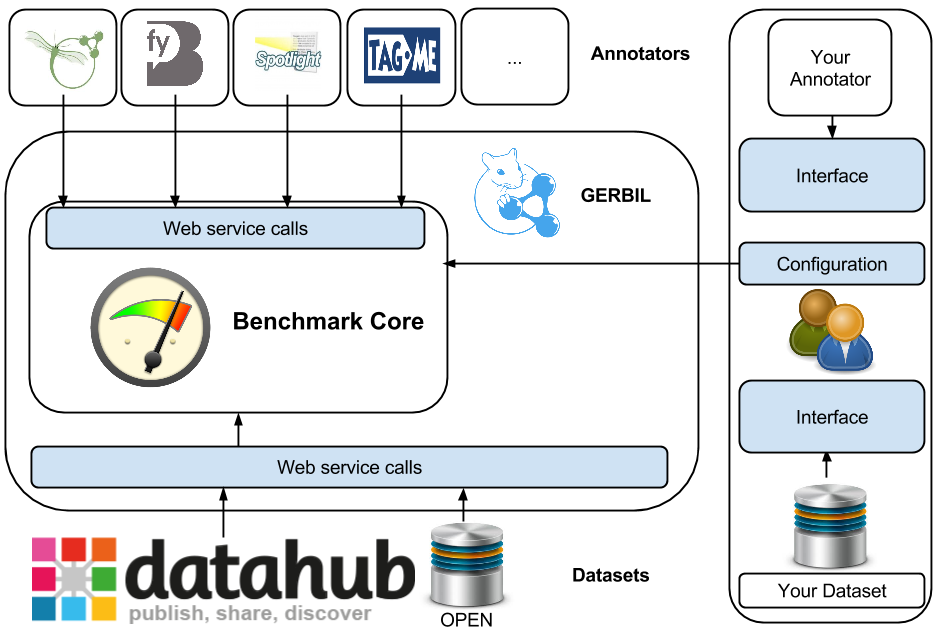
\includegraphics[width=0.6\linewidth]{GERBIL_new_architectur}
\caption{Overview of GERBIL's abstract architecture. Interfaces to users and providers of datasets and annotators are marked in blue.
%\todo[inline]{AnBo: Should the arrows/calls triggered from the core \emph{to}\ the datasets?}
}
\label{fig:architecture}
\end{figure*}

%Publishing, reproducing and archiving entity annotation results is a near-impossible endeavour.
%Finding and reusing datasets for comprehensive benchmarks involves often a trem\-endous amount of addition work.

\subsection{Architecture Overview}
GERBIL abides by a service-oriented architecture driven by the model-view-controller pattern (see Figure~\ref{fig:architecture}).
Entity annotation systems, datasets and configurations like experiment type, matching or metric are implemented as controller interfaces easily pluggable to the core controller. 
The output of experiments as well as descriptions of the various components are stored in a serverless database for fast deployment. % reachable from each controller. 
Finally, the view component displays configuration options respectively renders experiment results delivered by the main controller communication with the diverse interfaces and the database.

%\todo[inline]{AnBo: I have doubts regarding the buzzwords here. 1) A SOA needs a service repository providing callable interfaces to services but do not wrap the service. I am not sure what the actual implementation status is. Maybe we should take over the wording of our SEMANTiCS paper: oriented at the principles of service-oriented architectures. But maybe it is more closely to a plugin-architecture?
%2) Implementing a MVC pattern with distributed services is very complicated. Maybe a MVP pattern is a good description of the actual implementation?}
%\todo[inline]{How does GERBIL work internally? Short description of architecture needed}



% of fine grained measures to be able to cover a wide variety of experiments using diverse NER and NED approaches.
%GERBILs core is based on the endeavour of Cornolti et al.'s BAT-Framework~\cite{Cornolti} for comparing entity annotation systems. 

%\todo[inline]{(Andrea) We should add a table/image/example to clarify the different setups, even if some of them do not properly belong to the NED/EL/NEL/NER categories such as C2W, Sc2W and Rc2W which do not require the actual mention/entity mapping. Moreover, Sa2W and A2W can be seen as the same task assuming that the score for A2W systems is always equal to 1. (Ricardo): I agree with the last sentence. But that is how it is given in Cornoltis work. Furthermore, I would like to add a table mapping the approaches to categories. What do you think? And maybe add examples to the table below. (Andrea): which kind of categories? I don't think that examples for all the setups are really needed there should be only a single general example to make clear what EL is}
%postponed to M2 paper


\subsection{Features}
\label{sec:definitions}
%\todo[inline]{@Marco, Paolo/@Ricardo: please proof read this subsection}

%\begin{table*}[th]
\centering
\begin{tabular}{@{}p{3cm}p{2cm}p{3cm}p{7cm}@{}}
\toprule
Problem & Input & Output & Description \\ \midrule


Disambiguate to Wikipedia (D2KB) &
Text, Set of mentions &
Set of relevant annotations &
Assign to each input mention its pertinent entity (possibly null) \\ \midrule

Annotate to Wikipedia (A2KB) &
Text &
Set of relevant annotations &
Identify the relevant mentions in the input text and assign to each of them the pertinent entities \\ \midrule

Scored-annotate to Wikipedia (Sa2KB) &
Text &
Set of relevant and scored annotations &
As A2W, but here each annotation is assigned a score representing the likelihood that the annotation is correct \\ \midrule

Concepts to Wikipedia (C2KB) &
Text &
Set of relevant tags &
Tags are taken as the set of relevant entities that are mentioned in the input text \\ \midrule

Scored concepts to Wikipedia (Sc2KB) &
Text &
Set of relevant and scored tags &
As C2W, but here each tag is assigned a score representing the likelihood that the annotation is correct \\ \midrule

Ranked-concepts to Wikipedia (Rc2KB) &
Text &
Ranked list of relevant tags &
Identify the entities mentioned in a text and rank them in terms of their relevance for the topics dealt with in the
input text\\ \midrule

Classification/Typing to Wikipedia (T2KB) &
 &
 &
\\ \midrule

Entity Salience (ES2KB) &
  &
  &
\\\midrule

Entity Annotation/Detection (A) &
  &
  &
\\
\midrule
Word Sense Disambiguation (WSD) &
  &
  &
\\
\midrule
Relation Extraction (input text, predicate output: triple (BOA?) &
  &
  &\\
\bottomrule
\end{tabular}
\caption{Overview of the different task types.}
\label{tab:tasktypes}
\end{table*}

%\todo[inline]{add a table of mappings from tools to tasks}
%\todo[inline]{@Ricardo,Giuseppe,Micha, Axel: Discuss matchings (esp. TAC-KBP }
%postponed to M2
%\todo[inline]{(Ricardo) we need to discuss how to handle NIL entities while linking step, maybe consider measures from http://jhoff.de/wp-content/papercite-data/pdf/hoffart-2014hp.pdf. \\(Giuseppe) Whenever you refer to NIL then you are touching the TAC KBP EL/EDL effort somehow. There is already a consistent and mature body of work on that. I also encourage you to take a look at http://nlp.cs.rpi.edu/kbp/2014/KBP2014EL\_V1.1.pdf. The metrics proposed in TAC KBP already measure the effect of NIL links.}
%postponed to M2
%Here, we want to point to two import task types, i.e., D2W - disambiguation to Wikipedia which determines for each mention in a given set of mentions its pertinent entity~\cite{Cucerzan07} - and A2W - annotation to Wikipedia  which determines for a given unstructured text a set of relevant entities~\cite{milne2008learning}.
%'These problems can be casted in two main classes: the first consists of three problems which address the identification of (possibly scored) annotations, and thus the identification of mention-entity pairs; the second consists of three further problems that involve finding tags (possibly scored or ranked), thus accounting only for the entities.'
%For a detailed list of problems and their definition please have a look at the article itself~\cite{Cornolti}.

Experiments run in our framework can be configured in several manners. In the following, we present some of the most important parameters of experiments available in GERBIL. 

\subsubsection{Experiment types}
An experiment type defines the way used to solve a certain problem when extracting information.
Cornolti et al.'s~\cite{Cornolti} BAT-framework offers six different experiment types, namely (scored) annotation (S/A2KB), disambiguation (D2KB) -- also known as linking --, (scored respectively ranked) concept annotation (S/R/C2KB) of texts. 
In~\cite{rizzo2014}, the authors propose two types of experiments, focusing on highlighting the strengths and weaknesses of the analyzed systems.
Thereby, performing \textit{i)} entity recognition, i.e., the detection of the exact match of the pair entity mention and type (e.g., detecting the mention \textit{Barack Obama} and typing it as a \textit{Person}), and \textit{ii)} entity linking, where an exact match of the mention is given and the associated DBpedia URI has to be linked (e.g., locating a resource in DBpedia which describes the mention \textit{Barack Obama}).
This work differs from the previous one for experimenting in entity recognition, and on annotating entities to a RDF knowledge base.


% (Giuseppe)
%the flow I can get from here is: 
% - people worked on annotating (datasets, knowloedge bases): link or NIL
% - people worked on typing: fine grained (WEKEX, ACE,...) or coarse grained type (CoNLL: per,loc,org,...)
% - TAC KBP combines the two things, but it keeps the tasks in the simple form, i.e. typing only to a coarse grained schema (GPE, per, org) and using a sort-of knowldge base (their own creation of a set of wikipedia resource)
% next: 
% * going further and covering these issues (schemas, links)
% * domain adaptation analysis (Microposts2014 is about microposts, CoNLL is about newswire, etc etc)  
% (Ricardo)
% I guess, we should discuss next steps later, like after the deadline of WWW
% (Giuseppe) oki. But if we mention above the NERD efforts on experimenting NER, then we should claim something similar for GERBIL. Otherwise it's better removing that sentence

GERBIL reuses the six experiments provided by the BAT-framework and extends them by the idea to not only link to Wikipedia but to any knowledge base $K$.
%Thereby, we extend the idea of the before mentioned frameworks by introducing the concept of knowledge base-agnostic benchmarks.
%\todo[inline]{The following sentence does not make sense to me}
%That is, datasets and annotators are aware of their underlying knowledge bases, e.g., Wikipedia, DBpedia, Babelnet etc..
One major formal update of the measures in GERBIL is that in addition to implementing experiment types from previous frameworks, it also measures the influence of NIL annotations, i.e., the linking of entities that are recognized as such but cannot be linked to any resource from the reference knowledge base $K$. For example, the string \texttt{Ricardo Usbeck} can be recognized as a person name by several tools but cannot be linked to Wikipedia/DBpedia, as Ricardo does not have a URI in these reference datasets. 
Our framework extends the experiments types of~\cite{Cornolti} as follows: Let $m=(s,l,d,c) \in M$ denote an entity mention in document $d \in D$ with start position $s$, length $l$ and confidence score $c \in [0,1]$.
%that links to either a resource from the resource knowledge base $K$ or a global NIL entity if the entity mentioned is not in $K$. 
Note that some frameworks might not return (1) a position $s$ or a length $l$ for a mention, in which case we set $s=0$ and $l=0$; (2) a score $c$, in which case we set $c=1$.
%(Giuseppe) wikipedia is not a knowledge base. A knowledge base is a representation of the word for computing machinery, hence it has to be semantically structured. According to this definition, DBpedia is. Wikipedia is an encyclopedic resource, or simply a dataset
%\todo[inline]{AnBo@Ricardo: There is a problem with the definition of $m$, either it is $m=(s,l,d)$ without the score, or it has to be $m=(s,l,d,c,e)$ referring the resource e (that might NIL) mentioned in the description and needed for the score $c$. Note (Axel): The entity is given by a different function actually. Here, the tool only finds a mention (NER). NED occurs later :). Note (AnBo): But what expresses $c$ in this case?: Note (Axel): That's the confidence score for the mention.
%You are absolutely right. Just fixed it. It was simply incorrect. The mention must not link to an entity.
%(AnBo: perfect! issue closed.)
%}
%\todo[inline]{@axel,micha: discuss the below
%Old text: All the approaches mentioned in the last paragraphs work on Wikipedia page URIs or ids. 
%Since the introduction of DBpedia in 2007, new semantic approaches have been published based on unique DBpedia entity URIs instead of Wikipedia URIs. 
%Due to the bijective mapping, also older approaches can be used in GERBIL, which is more keen on Semantic Web technologies.
%}

%\todo[inline]{The following does not make any sense to a non-informed reader. The variables are simply not defined and used (see below). Stick to the formal definition of a mention above, which is incomplete, as it does not take $d$ into consideration.}
We implement six types of experiments:
\begin{enumerate}
\item \textbf{D2KB}: The goal of this experiment type is to map a set of \emph{given} entities mentions (i.e., a subset $\mu \subseteq M$) to entities from a given knowledge base or to NIL. Formally, this is equivalent to finding a mapping $a: \mu \rightarrow K \cup \{NIL\}$. In the classical setting for this task, the start position, the length and the score of the mentions $m_i$ are not taken into consideration. 
%The document for each entity is given explicitly. That's part of the formalization
%\todo[inline]{Micha: I don't understand the second sentence. Why is everything set to 0?. Axel: Fixed}
\item \textbf{A2KB}: This task is the classical NER/D task, thus an extension of the D2KB task. Here two functions are to be found. First, the entity mentions need to be extracted from a document set $D$. To this end, an extraction function $ex: D \rightarrow 2^M$ must be computed. The aim of the second step is then to match the results of $ex$ to entities from $K \cup \{NIL\}$ by devising a function $a$ as in the D2KB task.
%\todo[inline]{AnBo: I suggest a formal definition: $akin: m \rightarrow e$, where $e \in K \cup \{NIL\}$.Axel: akin is not a function}
%i.e.,  mapping a document $d$ to a set of entities $e_i \in K$ belonging to certain mentions $m_i(s_i,l_i)$ of this document. Formally, this is a mapping $a: d \rightarrow K \cup \{NIL\}$. The scores for those entities are ignored and thus $c_i=0$.
\item \textbf{Sa2KB}:
Sa2KB is an extension of A2KB where the scores $c_i \in [0,1]$ of the mentions detected by the approach are taken into consideration. These scores are then used during the evaluation.
\item \textbf{C2KB}: The concept tagging task C2KB aims to detect entities when given a document. Formally, the tagging function $tag$ simply returns a subset of $K$ for each input document $d$.
\item \textbf{Sc2KB}: This task is an extension of C2KB where the tagging function returns a subset of $K \times [0,1]$ for each input document $d$.
\item \textbf{Rc2KB}: In this particular extension of C2KB, the tagging function returns a sorted list of resources from $K$, i.e., an element of $K^*$, where $K^* = \bigcup\limits_{i=0}^\infty K^i$. 
\end{enumerate}

\begin{comment}
\begin{align}
\begin{split}
D2KB:&(d,K,\{m_1,\ldots,m_n\}) \rightarrow \{a_1,\ldots,a_n|\\
&a_i=(m_i,e_i), e_i\in K\cup\emptyset\}
\end{split}\\
\begin{split}
A2KB:&(d,K) \rightarrow \{a_1,\ldots,a_n|\\
&a_i=(s_i,l_i,e_i), e_i\in K\cup\emptyset, 0 < s_i \le |d|,\\
&0 < l_i, (s_i + l_i) \le |d|\}
\end{split}\\
\begin{split}
Sa2KB:&(d,K) \rightarrow \{a_1,\ldots,a_n|\\
&a_i=(s_i,l_i,e_i,c_i), e_i\in K\cup\emptyset, 0 < s_i \le |d|,\\
&0 < l_i, (s_i + l_i) \le |d|, 0 \le c_i \leq 1\}
\end{split}\\
\begin{split}
C2KB:&(d,K) \rightarrow \{e_1,\ldots,e_n|\\
&e_i\in K\cup\emptyset\}
\end{split}\\
\begin{split}
Rc2KB:&(d,K) \rightarrow \{a_1,\ldots,a_n|\\
&a_i=(e_i,r_i),e_i\in K\cup\emptyset,r \in [0,1]\}
\end{split}\\
\begin{split}
Sc2KB:&(d,K) \rightarrow \{a_1,\ldots,a_n|\\
&a_i=(e_i,c_i), e_i\in K\cup\emptyset, 0 \le c_i \leq 1\}
\end{split}
\end{align}
\end{comment}

With this extension, our framework can now deal with gold standard datasets and annotators that link to any knowledge base, e.g., DBpedia, BabelNet~\cite{NavigliPonzetto:12aij} etc., as long as the necessary identifiers are URIs.
We were thus able to implement \numberOfadditionalDatasets new gold standard datasets usable for each experiment type, cf. Section~\ref{sec:datasets}, and \numberOfadditionalAnnotators new annotators linking entities to any knowledge base instead of solely Wikipedia like in previous works, cf. Section~\ref{sec:annotators}.
With this extensible interface, GERBIL can be extended to deal with supplementary experiment types, e.g., entity salience~\cite{Cornolti}, entity detection~\cite{fox}, typing~\cite{rizzo2014}, word sense disambiguation (WSD)~\cite{babelfy} and relation extraction~\cite{fox}.
These categories of experiment types will be added to GERBIL in next versions.

%GERBIL leverages Linked Data usages for Benchmarks.

\subsubsection{Matching}

A matching defines which conditions the result of an annotator has to fulfill to be a correct result.
In case of existing redirections, we assume an implicit matching function to account for the many-to-one relation~\cite{Cornolti}.
The first matching type $M$ used for the C2KB, Rc2KB and Sc2KB experiments is the \textit{strong entity matching}.
Here, each mention is mapped to an entity of the knowledge base $K$ via a matching function $f$ with $f(m) \in K \cup \{NIL\}$.
Following this matching, a single entity mention $m = (s, l, d, c)$ returned by the annotator is correct iff it matches exactly with one of the entity mentions $m' = (s', l', d, c')$ in the gold standard $G(d)$ of d~\cite{Cornolti}. Formally,
\begin{align}
M(m,G)=
\begin{cases}
1 &  \text{iff }\exists m' \in G, f(m) = f(m'), \\
0 & \text{else.}
\end{cases}
\end{align}

For the D2KB experiments, the matching is expanded to the \textit{strong annotation matching} and includes the correct position of the entity mention inside the document.
\begin{align}
M_e(m,G) =
\begin{cases}
1 &  \text{iff }\exists m' \in G: f(m) = f(m') \wedge s = s' \wedge \\
  &l = l', \\
%&\quad s_g = s_a, l_g = l_a\\
0 & \text{else.}
\end{cases}
\end{align}

The strong annotation matching can be used for A2KB and Sa2KB experiments, too.
However, in practice this exact matching can be misleading.
A document can contain a gold standard named entity like "President Barack Obama" while the result of an annotator only marks "Barack Obama" as named entity.
Using an exact matching leads to weighting this result as wrong while a human might rate it as correct.
Therefore, the \textit{weak annotation matching} relaxes the conditions of the strong annotation matching.
Thus, a correct annotation has to be linked to the same entity and must overlap the annotation of the gold standard.

\begin{align}
M_w (m,G)=
\begin{cases}
1 &  \text{iff }\exists m' \in G, f(m) = f(m')  \land (\\
 &\ \ \ \,\, ( s \leq s' \land (s+l) \leq (s'+l') )\\ % left overlap
 &\ \ \lor ( s \geq s' \land (s+l) \geq (s'+l') )\\ % right overlap
 &\ \ \lor ( s \leq s' \land (s+l) \geq (s'+l') )\\ % outer overlap
 &\ \ \lor ( s \geq s' \land (s+l) \leq (s'+l') ))\\ % inner overlap
0 & \text{else.}
\end{cases}
\end{align}

%\todo[inline]{(RU) TAC-KBP?}
%postponed to M2
\newpage
\subsubsection{Metrics}
Currently, GERBIL offers six measures subdivided into two groups and derived from the BAT-framework, namely the micro- and the macro-group of precision, recall and f-measure.
%That is, macro measures are defined as average overall documents of the corresponding group measures while micro measures are calculated document-wise and averaged thereafter~\cite{Cornolti}.
At the moment, those measures ignore NIL annotations, i.e., if a gold standard dataset contains entities that are not contained in the target knowledge base $K$ and an annotator detects the entity and links it to any URI, emerging novel URI or NIL, this will always result in a false-positive evaluation. 
To alleviate this problem, GERBIL allows adding additional measures to evaluate the results of annotators regarding the heterogeneous landscape of gold standard datasets.

\subsubsection{Annotators}
\label{sec:annotators}

%The evaluation of different approaches for entity annotation can be a cumbersome endeavour due to various input and output formats, availability of source code, binaries or web services.
%GERBIL significantly reduces the amount of work required to compare existing as well as novel annotators in a comprehensive and reproducible way.
GERBIL aims to reduce the amount of work required to compare existing as well as novel annotators in a comprehensive and reproducible way. To this end, we provide two main approaches to evaluating entity annotation systems with GERBIL.
\begin{enumerate}
\item \textbf{BAT-framework Adapter}

Within BAT, annotators can be implemented by wrapping using a Java-based interface.
Since GERBIL is based on the BAT-framework, annotators of this framework can be added to GERBIL easily.
%GERBIL is based on the Spring framework\footnote{\url{http://spring.io/}} which led to a decrease of needed lines of code from on average XXX to XXX lines over the original BAT-framework.
%\todo[inline]{@Micha: Can we quantify that?\\ see latex comment}
%Micha: I don't think so. It depends on the system you want to call. And as I always say: lines of code is not a really good metric ;-) I do not even think that this is the correct position to argue with 1) GERBIL is Spring based (this simply doesn't matter) and 2) it is faster to implement - because GERBIL is still based on BAT, you have to implement exactly the same + a small overhead for getting the annotator into GERBIL. I think this time argument should be set to the NIF-based webservice, since you don't have to handle BAT-framework stuff there.
Due to the community effort behind GERBIL, we could raise the number of published annotators from 5 to \overallGERBILannotators.
We investigated the effort to implement a BAT-framework adapter in contrast to evaluation efforts done without a structured evaluation framework in Section~\ref{sec:eval}.

\item \textbf{NIF-based Services}:
GERBIL implements means to understand NIF-based~\cite{NIF} communication over web-service in two ways.
First, if the server-side implementation of annotators understands NIF-documents as input and output format, GERBIL and the framework can simply exchange NIF-documents.\footnote{We describe the exact requirements to the structure of the NIF document on our project website's wiki as NIF offers several ways to build a NIF-based document or corpus.}
%we can use a more simple and unified approach to bind new annotators into GERBIL.
Thus, novel NIF-based annotators can be deployed efficiently into GERBIL and use a more robust communication format compared to the amount of work necessary for deploying and writing a BAT-framework adapter.
%\todo[inline]{Here, I would argue that the implementation of a single NIF-webservice is faster than deploying the BAT-framework and implementing a BAT-framework adapter.}
Second, if developers do not want to publish their APIs or write source code, GERBIL offers the possibility for NIF-based webservices to be tested online by providing their URI and name only\footnote{\url{http://gerbil.aksw.org/gerbil/config}}. 
GERBIL does not store these connections in terms of API keys or URLs but still offers the opportunity of persistent experiment results.
%This web-based interface leverages the implementation of future annotators by offering a royalty-free annotation standard\footnote{\url{http://persistence.uni-leipzig.org/nlp2rdf/}}.
\end{enumerate}

Currently, GERBIL offers \overallGERBILannotators entity annotation systems with a variety of features, capabilities and experiments.
In the following, we present current state-of-the-art approaches both available or unavailable in GERBIL.
%For a list of available webservices, see Table~\ref{tab:annotator}.

%sorted by year
\begin{enumerate}
\item \textbf{Cucerzan}: As early as in 2007, Cucerzan presented a NED approach based on Wikipedia~\cite{Cucerzan07}. The approach tries to maximize the agreement between contextual information of input text and a Wikipedia page as well as category tags on the Wikipedia pages.
The test data is still available\footnote{\url{http://research.microsoft.com/en-us/um/people/silviu/WebAssistant/TestData/}} but since we can safely assume that the Wikipedia page content changed a lot since 2006, we do not use it in our framework, nor we are aware of any publication reusing this data.
Furthermore, we were not able to find a running webservice or source code for this approach.

\item \textbf{Wikipedia Miner}: This approach was introduced in~\cite{milne2008learning} in 2008 and is based on different facts like prior probabilities, context relatedness and quality, which are then combined and tuned using a classifier.
The authors evaluated their approach based on a subset of the AQUAINT dataset\footnote{\url{http://www.nist.gov/tac/data/data_desc.html\#AQUAINT}}.
They provide the source code for their approach as well as a webservice\footnote{\url{http://wikipedia-miner.cms.waikato.ac.nz/}} which is available in GERBIL.

\item \textbf{Illinois Wikifier}: In 2011, ~\cite{rat:rot} presented an NED approach for entities from Wikipedia. 
In this article, the authors compare local approaches, e.g., using string similarity, with global approaches, which use context information and lead finally to better results.
The authors provide their datasets\footnote{\url{http://cogcomp.cs.illinois.edu/page/resource_view/4}} as well as their software "Illionois Wikifier"\footnote{\url{http://cogcomp.cs.illinois.edu/page/software_view/33}} online.
Since "Illionois Wikifier" is currently only available as local binary and GERBIL is solely based on webservices we excluded it from GERBIL for the sake of comparability and server load.

\item \textbf{DBpedia Spotlight}: One of the first semantic approaches~\cite{spotlight}\ was published in 2011, this framework combines NER and NED approach based upon DBpedia\footnote{\url{https://github.com/dbpedia-spotlight/dbpedia-spotlight/wiki/Known-uses}}. 
%and acting as a central point for the Semantic Web community
Based on a vector-space representation of entities and using the cosine similarity, this approach has a public (NIF-based) webservice\footnote{\url{https://github.com/dbpedia-spotlight/dbpedia-spotlight/wiki/Web-service}} as well as its online available evaluation dataset\footnote{\url{http://wiki.dbpedia.org/spotlight/isemantics2011/evaluation}}.

\item \textbf{TagMe 2}: TagMe 2~\cite{TagMe2} was publised in 2012 and is based on a directory of links, pages and an inlink graph from Wikipedia.
The approach recognizes named entities by matching terms with Wikipedia link texts and disambiguates the match using the in-link graph and the page dataset.
Afterwards, TagMe 2 prunes identified named entities which are considered as non-coherent to the rest of the named entities in the input text.  
The authors publish a key-protected webservice\footnote{\url{http://tagme.di.unipi.it/}} as well as their datasets\footnote{\url{http://acube.di.unipi.it/tagme-dataset/}} online.
The source code, licensed under Apache 2 licence can be obtained directly from the authors.
%Unfortunately, their approach has two drawbacks: 
%(1) Texts with more than 3000 characters are a problem for the webservice. 
%Thus we slice longer texts near 3000 although there is the danger of cutting a named entity.
The datasets comprise only fragments of 30 words and less of full documents and will not be part of the current version of GERBIL. 
%\todo[inline]{drawback (1) is obselete as soon as we change to POST (2) is not a drawback directly.}

\item \textbf{AIDA}: The AIDA approach~\cite{AIDA} relies on coherence graph building and dense subgraph algorithms and is based on the YAGO2\footnote{\url{http://www.mpi-inf.mpg.de/yago-naga/yago/}} knowledge base.
%Specifically, this approach uses dense sub-graphs to identify coherent mentions using a greedy algorithm enabling Web scalability. 
Although the authors provide their source code, a webservice and their dataset which is a manually annotated subset of the 2003 CoNLL share task~\cite{conll2003}, GERBIL will not use the webservice since it is not stable enough for regular replication purposes.\footnote{\url{https://www.mpi-inf.mpg.de/departments/databases-and-information-systems/research/yago-naga/aida/}}

%\todo[inline]{@giuseppe: What is the Name of the approach, is it not available? than please delete it from table 2}
%van Erp et al.~\cite{vanErp2013,rizzo2014} have presented a NER approach tailored for microposts. They proposed a machine learning classification of the entity type given a rich feature vector composed of: a set of linguistic features, the output of a properly trained Conditional Random Fields classifier and the outputs of a set of off-the-shelf NER extractors. 
%Due to the unavailability of its source code or API van Erp et al.'s approach will not be part of GERBIL.
% The follow-up of van Erp's approach, NERD-ML, turns the entity recognition task as a classification task where the feature vector is based on a set of linguistic features, the output of a Condition Random Fields (CRF) properly trained, and the outputs of the annotation systems supported by the NERD Framework. This approach has shown strengths in both recognizing named entities in the newswire and the micropost domains~\cite{rizzo2014}.

\item \textbf{NERD-ML}: In 2013,~\cite{vanErp2013} proposed an approach for entity recognition tailored for extracting entities from tweets. The approach relies on a machine learning classification of the entity type given a rich feature vector composed of a set of linguistic features, the output of a properly trained Conditional Random Fields classifier and the output of a set of off-the-shelf NER extractors supported by the NERD Framework. The follow-up, NERD-ML~\cite{rizzo2014}, improved the classification task by re-designing the selection of the features, and they proposed experiments on both microposts and newswire domains.
NERD-ML has a public webservice which is part of GERBIL\footnote{\url{http://nerd.eurecom.fr/}}.


%too long in comparision
\item \textbf{KEA NER/NED}: This approach is the successor of the approach introduced in~\cite{Steinmetz2013} which is based on a fine-granular context model taking into account heterogeneous text sources %, as e.g. user tags, natural language texts, 
as well as text created by automated multimedia analysis. %, as e.g. automated speech recognition, optical character recognition, or visual concept detection. 
The source texts can have different levels of accuracy, completeness, granularity and reliability which influence the determination of the current context. 
Ambiguity is solved by selecting entity candidates with the highest level of probability according to the predetermined context. 
The new implementation begins with the detection of groups of consecutive words (n-gram analysis) and a lookup of all potential DBpedia candidate entities for each n-gram. 
The disambiguation of candidate entities is based on a scoring cascade. % including the analysis of connected components in the entity candidates' spanning sub-graphs in DBpedia, co-occurrence analysis with Wikipedia article texts, graph popularity measures (in-degree, pagerank)~\cite{dbpedia-graphmeasures}, as well as statistical and string distance metrics. 
%The final decision on the most likely entity candidate is determined with the help of machine learning classifiers, which is subject of current research. 
KEA is available as NIF-based webservice\footnote{\url{http://s16a.org/kea}}.


\item \textbf{WAT}: WAT is the successor of TagME~\cite{TagMe2}.\footnote{\url{http://github.com/nopper/wat}}
%, developed by Piccinno et al.~\cite{piccinno2014tagme} and was presented during the ERD Challenge~\cite{carmel2014erd}. 
%The project is released as an open source library\footnote{\url{http://github.com/nopper/wat}}. % and it is written in Scala. 
The new annotator includes a re-design of all TagME components, namely, the spotter, the disambiguator, and the pruner. 
Two disambiguation families were newly introduced: graph-based algorithms for collective entity linking based % (i.e., exploiting well-known graph algorithms such as PageRank, HITS and SALSA) 
and vote-based algorithms for local entity disambiguation (based on the work of Ferragina et al.~\cite{TagMe2}). 
The spotter and the pruner can be tuned using SVM linear models. 
Additionally, the library can be used as a D2KB-only system by feeding appropriate mention spans to the system. 
%commented because cornolti said it is not true. The system inherits some of the limitation of the legacy TagME~\cite{TagMe2}, i.e., being optimized for short texts. % (i.e. the spotter and the pruner modules are responsible for introducing many of the false positives).

\item \textbf{AGDISTIS}: This approach~\cite{AGDISTIS_ISWC} is a pure entity disambiguation approach (D2KB) based on string similarity measures, an expansion heuristic for labels to cope with co-referencing and the graph-based HITS algorithm.
The authors published datasets\footnote{\url{https://github.com/AKSW/n3-collection}} along with their source code and an API\footnote{\url{https://github.com/AKSW/AGDISTIS}}.
AGDISTIS can only be used for the D2KB task.

\item \textbf{Babelfy}: The core of this approach lies in the use of random walks and a densest subgraph algorithm to tackle the word sense disambiguation and entity linking tasks in a multilingual setting~\cite{babelfy} thanks to the BabelNet semantic network~\cite{NavigliPonzetto:12aij}.
Babelfy has been evaluated using six datasets: three from earlier SemEval tasks \cite{pradhan2007semeval,NavigliLH:2007,Naviglietal:13}, one from a Senseval task \cite{snyder2004english} and two already used for evaluating AIDA \cite{AIDA,HoffartSNTW:2012}.
All of them are available online but distributed throughout the web. 
Additionally, the authors offer a webservice limited to 100 requests per day which are extensible for research purposes\footnote{\url{http://babelfy.org}} \cite{BabelfyAPI}.

%\todo[inline]{@diego(?): describe DEXTER here, and update all tables}

\item \textbf{Dexter}: This approach \cite{ceccarelli2013dexter} is an open-source implementation of an entity disambiguation framework.
The system was implemented in order to simplify the implementation of an entity linking approach and allows to replace single parts of the process.
%It runs on commodity hardware and requires only 3 gigabytes of memory.
The authors implemented several state-of-the-art disambiguation methods.
Results in this paper are obtained using an implementation of the original TagMe disambiguation function.
Moreover, Ceccarelli et al. provide the source code\footnote{\url{http://dexter.isti.cnr.it}} as well as a webservice.
\end{enumerate}

Table~\ref{tab:annotator} compares the implemented annotation systems of GERBIL and the BAT-Framework.
While AGDISTIS has been in the source code of the BAT-Framework provided by a third-party after publication of Cornolti et al.'s initial work~\cite{Cornolti} in 2014, GERBIL's community effort led to the implementation of overall \numberOfadditionalAnnotators new annotators as well as the before mentioned generic NIF-based annotator.
The AIDA annotator as well as the "Illinois Wikifier" will not be available in GERBIL since we restrict ourselves to webservices.
However, these algorithms can be integrated at any time as soon as their webservices are available.
%\todo[inline]{@Micha: bitte nochmal alle tabellen anschauen :)}
%\todo[inline]{@Giuseppe: NERD-ML is not described above. could you please do that? and afterwards update all tables and clarify whether van erp is an own approach}

\begin{table}[htb]
\centering
\begin{tabulary}{\columnwidth}{LLCCC}
\toprule
                                        && BAT-Framework           & GERBIL                    & Experiment\\ 
\midrule
\multirow{2}{*}{\cite{milne2008learning}}&Wikipedia Miner& \multirow{2}{*}{\haken} & \multirow{2}{*}{\haken}   & \multirow{2}{*}{SA2KB}\\
\multirow{2}{*}{\cite{rat:rot}}&Illionois Wikifier       & \multirow{2}{*}{\haken} & \multirow{2}{*}{(\haken)} & \multirow{2}{*}{SA2KB}\\
\cite{spotlight}&Spotlight             & \haken                  & \haken                    & SA2KB\\
\cite{TagMe2}&TagMe 2                   & \haken                  & \haken                    & SA2KB\\
\cite{AIDA}&AIDA                        & \haken                  & (\haken)                  & SA2KB\\
%&van Erp?                                &                         & ?                         &\\
\cite{Steinmetz2013}&KEA                &                         & \haken                    & SA2KB\\
\cite{piccinno2014tagme}&WAT            &                         & \haken                    & SA2KB\\
\cite{AGDISTIS_ISWC}&AGDISTIS           & (\haken)                & \haken                    & D2KB\\
\cite{babelfy}&Babelfy                  &                         & \haken                    & SA2KB\\
\cite{rizzo2014}&NERD-ML                &                         & \haken                    & SA2KB\\
\cite{ceccarelli2013dexter}&Dexter &                         & \haken                    & SA2KB\\
&NIF-based Annotator                     &                         & \multirow{2}{*}{\haken}   & \multirow{2}{*}{any}\\
\bottomrule
\end{tabulary}
\caption{Overview of implemented annotator systems. Brackets indicate the existence of the implementation of the adapter but also the inability to use it in the live system.}
\label{tab:annotator}
\end{table}

%\subsection{Front-end}
%Our web-based frontend provides opportunities to handle a number of different use cases as described in Section~\ref{sec:usecase}.
%Especially, we tried to offer each configuration available in the programmatic backend also to frontend-users.
%Especially, we provide users with long-term stable URIs for their chosen configuration, see also Section~\ref{sec:longtermstability}.
%\todo[inline]{Add screenshot}

\subsection{Datasets}
\label{sec:datasets}
%\todo[inline]{(Giuseppe) pls check: ambiguity in naming the AIDA CoNLL-YAGO Dataset. -> AIDA/CoNLL}

Table~\ref{tab:datasetformats} shows the heterogeneity of datasets used for prior evaluations while Table~\ref{tab:datasets} presents an overview of the datasets that were used to evaluate some well-known entity annotators in previous works.
These tables make clear that the numbers and types of used datasets varies a lot, thus preventing a fast comparison of annotation systems.

%GERBIL's main goal is the improvement of the reproducibility of entity annotation experiments. 
%Thus, our approach offers the opportunity to easily compare a wealth of entity annotations systems and various datasets with diverse experiment and matching types as well as metrics, cf. .
\begin{table}[htb]
\centering
\begin{tabulary}{\columnwidth}{LCC}
\toprule
Dataset                 & Format    & Experiment\\
\toprule
ACE2004                 & MSNBC     & Sa2KB\\
Wiki                    & $\star$   & Sa2W \\
Aquaint                 & $\star$   & Sa2KB\\
MSNBC                   & MSNBC     & Sa2KB\\
IITB                    & XML       & Sa2KB\\
Meij                    & TREC      & Rc2W \\
AIDA/CoNLL              & CoNLL     & Sa2KB \\
N$^3$ collection        & NIF/RDF   & Sa2KB \\
KORE 50                 & NIF/RDF   & Sa2KB \\
Wiki-Disamb30           & tab-separated & Sa2KB \\
Wiki-Annot30            & tab-separated & Sa2KB \\
Spotlight Corpus        & NIF/RDF   & Sa2KB \\
SemEval-2013 task 12    & XML/$\star$&WSD/Sa2KB\\
SemEval-2007 task 7     & XML/$\star$&WSD\\
SemEval-2007 task 17    & XML/$\star$&WSD\\
Senseval-3              & XML/$\star$&WSD\\
Microposts2014          & Microposts2014 & Sa2KB\\
\bottomrule
\end{tabulary}
\caption{Datasets and their formats. A $\star$ indicates various inline or keyfile annotation formats. The experiments follow their definition in Section~\ref{sec:definitions}}
\label{tab:datasetformats}
\end{table}



\begin{table}[tb!]
\centering
 \resizebox{\textwidth}{!}{ 
\begin{tabular}{lccccccccccccccccccc|cc}
\toprule
                   & \rot{Year} & \rot{ACE} & \rot{Wiki} & \rot{Aquaint} & \rot{MSNBC} & \rot{IITB} & \rot{Meij} & \rot{AIDA/CoNLL} & \rot{N$^3$ collection} & \rot{KORE 50} & \rot{Wiki-Disamb30} & \rot{Wiki-Annot30} & \rot{Spotlight Corpus} & \rot{SemEval-2013 task 12} & \rot{SemEval-2007 task 7} & \rot{SemEval-2007 task 17} & \rot{Senseval-3} & \rot{NIF-based corpus} & \rot{Microposts2014} & \rot{Software available?} & \rot{Web service available?} \\ \midrule
Cucerzan & 2007 & & & & \haken & & & & & & & & & & & & & & & \\
%Wikipedia Miner gets a new line --> we put it in two lines to center the cells vertically
Wikipedia & \multirow{2}{*}{2008} & & & \multirow{2}{*}{\haken*} & & & & & & & & & & & & & & & & & \multirow{2}{*}{\haken} \\
Miner &&&&&&&&&&&&&&&&&&&&&\\
\mbox{Illionois Wikifier} & 2011 & \haken & \haken & \haken* & \haken & & & & & & & & & & & & & & & \haken & \\
Spotlight & 2011 & & & & & & & & & & & & \haken & & & & & & & \haken & \haken \\
AIDA & 2011 & & & & & & & \haken & & & & & & & & & & & & \haken & \haken** \\
TagMe 2  & 2012 & & & & & & & & & & \haken & \haken & & & & & & & & \haken & \haken \\
Dexter & 2013 & & & & & & & & & & & & & & & & & & & \haken & \haken \\
KEA & 2013 & & & & & & & & & & & & & & & & & & &  & \haken \\
WAT & 2013 & & & & & & & & & & & & & & & & & & &  \haken & \haken \\

AGDISTIS & 2014 & & & \haken & \haken & \haken & \haken & \haken & \haken & \haken & & & \haken & & & & & & & \haken & \haken \\
Babelfy & 2014 & & & & & & & \haken & & \haken & & & & \haken & \haken & \haken & \haken & & & & \haken \\
\mbox{NERD-ML} & 2014 & & & & & & & \haken & & & & & & & & & & & \haken & \haken & \haken \\
\midrule
BAT- & \multirow{2}{*}{2013} & \multirow{2}{*}{\haken} & \multirow{2}{*}{\haken} & \multirow{2}{*}{\haken} & \multirow{2}{*}{\haken} & \multirow{2}{*}{\haken} & \multirow{2}{*}{\haken} & \multirow{2}{*}{\haken*} & & & & & & & & & & & & \multirow{2}{*}{\haken} & \\
\mbox{Framework} &&&&&&&&&&&&&&&&&&&&&\\
NERD & \multirow{2}{*}{2014} & & & & & & \multirow{2}{*}{\haken} & \multirow{2}{*}{\haken} & & & & & & & & & & & \multirow{2}{*}{\haken} & \multirow{2}{*}{\haken} & \multirow{2}{*}{\haken} \\
\mbox{Framework} &&&&&&&&&&&&&&&&&&&&&\\
GERBIL & 2014 & \haken & \haken & \haken & \haken & \haken & \haken & \haken* & \haken & \haken &  & & \haken &  & & & & \haken & \haken  & \haken & \haken \\ 
\bottomrule
\end{tabular}
}
\caption{Comparison of annotators and datasets with indication whether software or datasets respectively Web services are available for reproduction. $*$ indicates that only a subset has been used to evaluate this annotator.
$**$ indicate that the Web service is not meant to be used within scientific evaluations due to unstable backends.}
\label{tab:datasets}
\end{table}

BAT allows evaluating the performance of different a\-ppro\-aches using five datasets, namely AQUAINT, MSNBC, IITB, Meij and AIDA/CoNLL.
With GERBIL, we activate one more dataset already implemented by the authors, namely ACE2004 from Ratinov et al.~\cite{rat:rot}.
Furthermore, we implemented a dataset wrapper for the Microposts2014 corpus which has been used to evaluate NERD-ML~\cite{rizzo2014}. 
The dataset itself was introduced in 2014~\cite{Cano2014} and consists of 3500 tweets especially related to event data.
Moreover, we capitalize upon the uptake of publicly available, NIF based corpora over the last years~\cite{yovisto,N3}\footnote{\url{http://datahub.io/dataset?license_id=cc-by&q=NIF}}.
To this end, GERBIL implements a Java-based NIF~\cite{NIF} reader and writer module which enables loading arbitrary NIF document collections, as well as the communication to NIF-based webservices.
Additionally, we integrated four NIF corpora, i.e., the RSS-500 and reuters-128 dataset\footnote{\url{https://github.com/AKSW/n3-collection}}, as well as the Spotlight Corpus and the KORE 50 dataset\footnote{\url{http://www.yovisto.com/labs/ner-benchmarks/}}. 

The extensibility of the datasets in GERBIL is furthermore ensured by allowing users to upload or use already available NIF datasets from DataHub. 
GERBIL will regularly check whether new corpora are available and publish them for benchmarking after a manual quality assurance cycle which ensures their usability for the implemented configuration options.
Additionally, users can upload their NIF-corpora directly to GERBIL avoiding their publication in publicly available sources.
This option allows for rapid testing of entity annotation systems with closed source or licenced datasets.

Some of the datasets shown in Table~\ref{tab:datasets} are either not yet implemented due to size and server load limitations, i.e., Wiki-Disamb30 and Wiki-Annot30, or due their original experiment type.
In particular, the Senseval-3 as well as the different SemEval datasets demand as experiment type word sense disambiguation and thereby linking to BabelNet or Wordnet~\cite{Wordnet}, which is not yet covered in GERBIL.
Still, GERBIL offers currently \overalldatasets state-of-the-art datasets reaching from newswire and twitter to encyclopedic corpora of various amounts of texts and entities.
Due to license issues we are only able to provide downloads for 9 of them directly but we provide instructions to obtain the others on our project wiki.

Table~\ref{tab:corpus_stats} depicts the features of the current datasets available in GERBIL.
These provide a broad evaluation ground leveraging the possibility for sophisticated tool diagnostics.

%\todo[inline]{@AKSW:  output statistics for all available corpora, i.e., nr of docs, nr of entities, length of documents, domain as table thx.}

\begin{table*}
    \begin{tabular}{lp{0.25cm}rp{0.25cm}rp{0.25cm}r}
     \toprule
     Corpus && Topic && \multicolumn{1}{c}{$\left|\text{Documents}\right|$} && \multicolumn{1}{c}{Avg. Entity/Doc.} \\
    \midrule
ACE2004          && news            &&   57 &&   4.44\\
AIDA/CoNLL       && news            && 1393 &&  19.97\\
Aquaint          && news            &&   50 &&  14.54\\
IITB             && mixed           &&  103 && 109.22\\
KORE 50          && mixed           &&   50 &&   2.86\\
Meij             && tweets          &&  502 &&   1.62\\
Microposts2014   && tweets          && 3505 &&   0.65\\
MSNBC            && news            &&   20 &&  32.50\\
N$^3$ Reuters-128&& news            &&  128 &&   4.85\\
N$^3$ RSS-500    && RSS-feeds       &&  500 &&   0.99\\
Spotlight Corpus && news            &&   58 &&   5.69\\
%Wiki             && encyclopedic    &&   ? &&   ?\\
	\bottomrule
	\end{tabular}
	\centering
    \caption{Features of the datasets and their documents.}
	\label{tab:corpus_stats}
\end{table*}

\subsection{Output}
\label{sec:output}
GERBIL's main aim is to provide comprehensive, reproducible and publishable experiment results.
Hence, GERBIL's experimental output is represented as a table containing the results, as well as embedded JSON-LD\footnote{\url{http://www.w3.org/TR/json-ld/}} RDF data using the RDF DataCube vocabulary~\cite{datacube}.
We ensure a detailed description of each component of an experiment as well as machine-readable, interlinkable results following the 5-star Linked Data principles.
Moreover, we provide a persistent and time-stamped URL for each experiment, see Table~\ref{tab:persistentURL}.

\begin{table}
    \begin{tabular}{lcr}
    \toprule
    Annotator & Dataset & F1-micro \\
    \midrule
    DBpedia Spotlight & IITB & 0.444 \\
    Babelfy & IITB & 0.377 \\
    NERD-ML & IITB & 0.488 \\
    WAT & IITB & 0.202 \\
    DBpedia Spotlight & KORE50 & 0.265 \\
    Babelfy & KORE50 & 0.476 \\
    NERD-ML & KORE50 & 0.238 \\
    WAT & KORE50 & 0.523 \\
	\bottomrule
	\end{tabular}
	\centering
    \caption{Results of an example experiment. It is accessible at \url{http://gerbil.aksw.org/gerbil/experiment?id=201411100001}}
	\label{tab:persistentURL}
\end{table}
%\todo[inline]{Add URL}

\emph{RDF DataCube} is a vocabulary standard and can be used to represent fine-grained multidimensional, statistical data which is compatible with the  Linked SDMX~\cite{LinkedSDMX} standard. 
Every GERBIL experiment is modelled as \texttt{qb:Dataset} containing the individual runs of the annotators on specific corpora as \texttt{qb:Observations}. 
Each observation features the \texttt{qb:Dimensions} experiment type, matching type, annotator, corpus and time. 
The six evaluation measures offered by GERBIL as well as the error count are expressed as \texttt{qb:Measures}. 
To include further metadata, annotator and corpus dimension properties link \emph{DataID}~\cite{dataID} descriptions of the individual components. 

GERBIL uses the recently proposed DataID~\cite{dataID} ontology that combines VoID~\cite{void} and DCAT~\cite{dcat} metadata with Prov-O~\cite{prov-o} provenance information and ODRL~\cite{odrl} licenses to describe datasets.
Besides metadata properties like titles, descriptions and authors, the source files of the open datasets themselves are linked as \texttt{dcat:Distributions}, allowing direct access to the evaluation corpora. 
Furthermore, ODRL license specifications in RDF are linked via \texttt{dc:license}, potentially facilitating automatically adjusted processing of licensed data by NLP tools. 
Licenses are further specified via \texttt{dc:rights}, including citations of the relevant publications. 

To describe annotators in a similar fashion, we extended DataID for services. 
The class \texttt{Service}, to be described with the same basic properties as dataset, was introduced. 
To link an instance of a \texttt{Service} to its distribution the \texttt{datid:distribution} property was introduced as super property of \texttt{dcat:distribution}, i.e., the specific URI the service can be queried at.
Furthermore, Services can have a number of \texttt{datid:Parameters} and \texttt{datid:Configurations}.
Datasets can be linked via \texttt{datid:input} or \texttt{datid:output}. 

Offering such detailed and structured experimental results opens new research avenues in terms of tool and dataset diagnostics to increase decision makers' ability to choose the right settings for the right use case.
Next to individual configurable experiments, GERBIL offers an overview of recent experiment results belonging to the same experiment and matching type in the form of a table as well as sophisticated visualizations\footnote{\url{http://gerbil.aksw.org/gerbil/overview}}, see Figure~\ref{fig:spider}.
This allows for a quick comparison of tools and datasets on recently run experiments without additional computational effort.

\begin{figure}[htb]
\centering
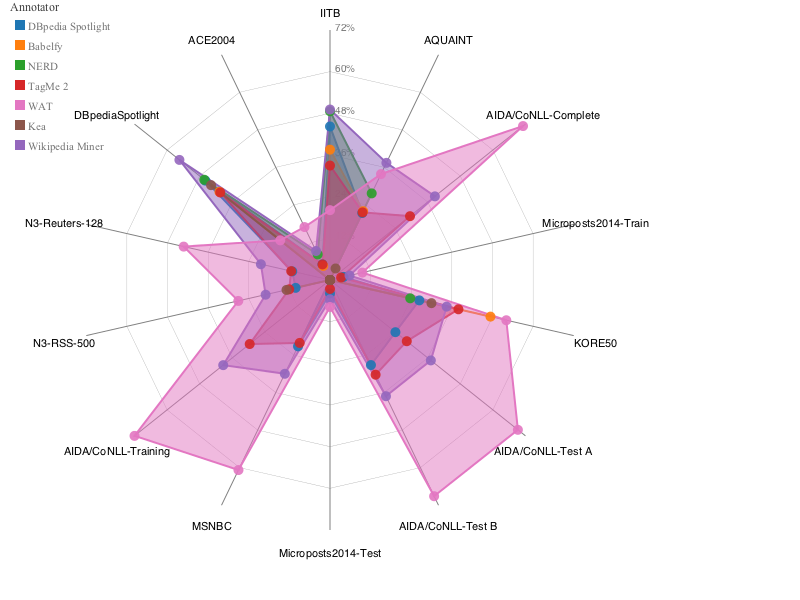
\includegraphics[width=0.5\textwidth]{spider}
\caption{Example spider diagram of recent A2KB experiments with strong annotation matching derived from our online interface}
\label{fig:spider}
\end{figure}



\section{Evaluation}
\label{sec:eval}
%GERBIL allows publishing, citing, reproducing and analysing entity annotation experiment data.

To ensure the practicability and convenience of the GERBIL framework, we investigated the effort needed to use GERBIL for the evaluation of novel annotators.
To achieve this goal, we surveyed the workload necessary to implement a novel annotator into GERBIL compared to the implementation into previous diverse frameworks.

Our survey comprised five developers with expert-level programming skills in Java. Each developer was asked to evaluate how much time he/she needed to write the code necessary to evaluate his/her framework on a new dataset.

%\todo[inline]{Add diagram showing time for own data/time on GERBIL}
\begin{figure}
\centering
\includegraphics[width=\columnwidth]{user_study.eps}
\caption{Comparison of effort needed to implement an adapter for an annotation system with and without GERBIL.}
\label{ref:comparedTime}
\end{figure}


Overall, the developers reported that they needed between 1 and 4 hours to achieve this goal (4x 1-2h, 1x 3-4h), see Figure~\ref{ref:comparedTime}.
Importantly, all developers reported that they needed either the same or even less time to integrate their annotator into GERBIL.
This result in itself is of high practical significance as it means that by using GERBIL, developers can evaluate on (currently) \overalldatasets datasets using the same effort they needed for 1, which is a gain of more than 1100\%.
Moreover, all developers reported they felt comfortable---4 points on average on a 5-point Likert scale between very uncomfortable (1) and very comfortable (5)---implementing the annotator in GERBIL.
Further developers were invited to complete the survey, which is available at our project website.
%\url{ https://docs.google.com/spreadsheets/d/1v3EyAnHxA3zgfoL4CcqEM4_EbvpKiCWeg6qc3FOKf2o/edit#gid=414618098}
Even though small, this evaluation suggests that implementing against GERBIL does not lead to any overhead. On the contrary, GERBIL significantly improves the time-to-evaluation by offering means to benchmark and compare against other annotators respectively datasets within the same effort frame previously required to evaluate on a single dataset.

An interesting side-effect of having all these frameworks and datasets in a central framework is that we can now benchmark the different frameworks with respect to their runtimes within exactly the same experimental settings. These results are of practical concern for end users of annotation frameworks as they are most commonly interested in both the runtime and the quality of solutions. For example, we evaluated the runtimes of the different approaches in GERBIL for the A2KB experiment type on the MSNBC dataset. The results of this experiment are shown in Figure~\ref{fig:runtime}.


\begin{figure}[htb]
\centering
\includegraphics[width=\columnwidth]{needed_times.eps}
\caption{Runtime per document of different approaches in GERBIL for the A2KB experiment type on the MSNBC dataset.}
\label{fig:runtime}
\end{figure}
%\todo[inline]{@Micha runtime in s/document?}

%\subsection{Reproducibility of experiments}
%\label{sec:repro}
%\todo[inline]{ADD A2W, D2W benchmark tables here with URIs to proof GERBIL %works.}
%The main goal of GERBIL is to provide comprehensible experiments in the field of NER and NED.
%Especially, we are interested in reproducing the results of AGDISTIS~\cite{AGDISTIS_ISWC}, TagMe 2~\cite{TagMe2,Cornolti} and Babelfy~\cite{babelfy}.

\section{Conclusion and Future Work}
\label{sec:conclusion}
In this paper, we presented and evaluated GERBIL, a platform for the evaluation of annotation frameworks. With GERBIL, we aim to push annotation system developers to better quality and wider use of their frameworks.
Some of the main contributions of GERBIL include the provision of persistent URLs for reproducibility and archiving.
Furthermore, we implemented a generic adaptor for external datasets as well as a generic interface to integrate remote annotator systems.
The datasets available for evaluation in the previous benchmarking platforms for annotation was extended by \numberOfadditionalDatasets new datasets. Moreover, \numberOfadditionalAnnotators novel annotators were added to the platform. 
The evaluation of our framework by contributors suggests that adding an annotator to GERBIL demands 1 to 2 hours of work. Hence, while keeping the implementation effort previously required to evaluate on a single dataset, we allow developers to evaluate on (currently) \overalldatasets times more datasets.
The presented, web-based frontend allows for several use cases enabling laymen and expert users to perform informed  comparisons of semantic annotation tools.
The persistent URIs enhances the long term quotation in the field of information extraction.
GERBIL is not just a new framework wrapping existing technology. 
In comparison to earlier frameworks, it extends the state-of-the-art benchmarks by the capability of considering the influence of NIL attributes and the ability of dealing with data sets and annotators that link to different knowledge bases.
%GERBIL is being updated continuously.
More information about GERBIL and its source code can be found at the project's website. 

%\todo[inline]{AnBo: Currently it sound like a wrapper framework for convenient programming. I would add the functional evolution comparing BAT as well. Suggestion:

%However, GERBIL is not just a new framework wrapping existing technology. 
%In comparison to earlier frameworks, it extends the state-of-the-art benchmarks by the capability of considering the influence of NIL attributes and the ability of dealing with data sets and annotators that link to different knowledge bases.
%AN: Done
%}

While developing GERBIL, we spotted several flaws in the formal model underlying previous benchmarking frameworks which we aim to tackle in the future. 
For example, the formal specification underlying current benchmarking frameworks for annotation does not allow using the scores assigned by the annotators for their results. To address this problem, we aim to develop/implement novel measures into GERBIL that make use of scores (e.g., Mean Reciprocal Rank). 
Moreover, partial results are not considered within the evaluation. For example, during the disambiguation task, named entities without Wikipedia URIs are not considered. This has a significant impact of the number of true and false positives and thus on the performance of some tools.
Furthermore, certain tasks seem to be too coarse. For example, we will consider splitting the Sa2KB and the A2KB tasks into two subtasks: The first subtask would measure how well tools perform at finding named entities inside the text (NER task) while the second would evaluate how well tools disambiguate those named entities which have been found correctly (similar to the D2KB task).
In the future, we also plan to provide information about the point in time since when an annotator is stable, i.e., the algorithm underlying the webservice has not changed.
%All the above mentioned points will be intensively discussed and implemented in a new version of GERBIL.

\begin{wrapfigure}[4]{r}{0.18\textwidth}
% \vspace{-8mm}
 
\includegraphics[width=0.18\textwidth]{esf.pdf}
\end{wrapfigure}
\textbf{Acknowledgments.} Parts of this work were supported by the ESF and the Free State of Saxony, the FP7 projects GeoKnow (GA No. 318159), LIDER (GA No. 610782), and LinkedTV (GA No. 287911).

\bibliographystyle{abbrv}
\bibliography{myrefs}
%\appendix

\balancecolumns

\begin{comment}
\todo[inline]{@All: Need to decide whether we really need the section below. Seems redundant.}
\section{Appendix: Using GERBIL}
\label{sec:usecase}
In the following, we present some use-case scenarios for our framework.

\subsection{Look Up of already published experiments}
Compliant with the main goal of GERBIL the reproduction of a certain experiment is central to facilitating research efforts. %, e.g., those published in \cite{AGDISTIS_ISWC,AIDA,TagMe2,babelfy}.
Therefore, our web-based platform offers the opportunity to configure an experiment using the parameters defined in Section~\ref{sec:architecture}.
The results will be displayed as described in Section~\ref{sec:output} and the experiment itself has a time-stamped URL which is citable and will be stable over time smoothing the way to a new citation quality.

\subsection{Evaluation of novel open-source datasets}

GERBIL is designed to be extensible, especially w.r.t. novel datasets.
Therefore, we differentiate three ways of integrating such datasets.
(1) A user can upload a NIF-based corpus of documents via our web-interface.
(2) GERBIL downloads datasets from \url{datahub.io} which we will then pull via HTTP requests which will be available after manual revision.
(3) Users can also implement a new dataset wrapper source code-wise. 
If users than decide to integrate their wrappers intp GERBILs public repository the community will be further-on able to use it for public evaluations. 
%Afterwards, we will revise the source code and add it to the set of public datasets.

\subsection{Submitting a closed-source dataset}

GERBIL also provides an opportunity for closed source data\-set evaluation, e.g., business-relevant data or just experimental data not yet ready to be published.
Users can upload their NIF-based dataset via GERBILs web interface.
Apart from the experiment results calculated with it, GERBIL will keep \emph{no} other data of such a dataset.

\subsection{Submitting a new algorithm (open or closed source)}

Finally, users can submit new webservice-based entity annotation systems in two different ways:
(1) By providing us with the necessary information to call their NIF-based webservice.
Thereby, they need to enter the webservice's URI and a name for the algorithm.
This methods enables fast prototyping of webservices without the need to implement a BAT-framework annotator wrapper.
To lower barriers, we provide a NIF converter in Java.
(2) Additionally, a user can use our source code project, implement a new annotator and push his source code back to us. 
After a feasibility check, we will then bring the enhanced version of GERBIL online and announce it on the website.
Thus, a tremendous gain with respect to possible comparison opportunities in terms of annotators and datasets is inflicted.



%by providing annotator evaluation and  to the Semantic Web providing not only a mapping to Wikipedia sites, but also to DBpedia URIs, which has not been possible with the underlying framework yet. 


%In future work, enable the use of local algorithms such as AIDA and illonois wikifier}
%First, several frameworks work solelonly with Wikipedia URIs/identifiers which hinders the use of other databases as background knowledge. 
%A better solution would only use arbitrary URIs which will be matched between a dataset and an annotated result.


%(3) The BAT-framework aborts the benchmarking process if the annotator returns an error. While this might be a reasonable behavior, it is annoying for developers that want to know the status of their prototype or the performance of other annotators on their data. 
%During the processing of external data or working with external annotators there will always be smallish problems like encoding errors. 
%Therefore, we want to refactor this behaviour in the source code to return the number of errors that had happened during the annotation process.
%(4) Finally, the BAT-Framework removes annotations which have no disambiguated Wikipedia URIs from the datasets.
%This is, the number of true/false negatives is significantly influenced by the framework and valuable information are lost.


%This article presents GERBIL, a generalised entity annotation framework which we extended by a new annotator for Babelfy and activated another - AGDISTIS - for new comparisons.
\end{comment}


\end{document}
%\documentclass{llncs}

%\usepackage{graphicx}
%\usepackage{pifont}
%\usepackage{amsmath,amssymb}
%\usepackage[english]{babel}
%\usepackage[utf8]{inputenc}
%\usepackage[ruled,vlined]{algorithm2e}
%\usepackage{hyperref}
%\usepackage{float} 
%\usepackage{multirow} 
%\usepackage{booktabs}
%\usepackage[disable]{todonotes}
%\usepackage{todonotes}
%\usepackage{mdframed}
%\usepackage{wrapfig}
%\usepackage{booktabs}
%\usepackage{cha333:tabulary}
%\usepackage{caption}
%\usepackage{comment}
%\usepackage{tikz}
%\usepackage{xspace}
%\usepackage{times}
%\usepackage{subfigure}

%\newcommand{\haken}{{\ding{51}}}
%\newcommand*\rot{\rotatebox{87}}



%\begin{document}

\chapter{Evaluating Entity Annotators Using GERBIL}

%\author{
%Ricardo Usbeck \and 
%Michael Röder \and
%Axel-Cyrille Ngonga Ngomo
%}

%\institute{
%University of Leipzig, Germany\\\email{\{usbeck,roeder,ngonga\}@informatik.uni-leipzig.de}
%}

%\maketitle

%\begin{abstract}
The need to bridge between the unstructured data on the Document Web and the structured data on the Web of Data has led to the development of a considerable number of annotation tools. However, these tools are hard to compare due to the diversity of data sets and measures used for evaluation. 
We will demonstrate GERBIL, an evaluation framework for semantic entity annotation that provides developers, end users and researchers with easy-to-use interfaces for the agile, fine-grained and uniform evaluation of annotation tools on 11 different data sets within 6 different experimental settings on 6 different measures. 
%We present the different types of experiments as well as the human-readable and machine-readable output formats supported by GERBIL. In addition, we show how the permanent experiment URIs provided by GERBIL ensure the reproducibility and archiving of evaluation results. Finally, we show how GERBIL can provide developers with diagnostics that allow to spot current strengths and weaknesses of their annotators. 
%\end{abstract}


\section{Introduction}
%The implementation of the original vision behind the Semantic Web demands the development of approaches and frameworks for the seamless extraction of structured data from text. 
The need for extracting structured data from text has led to the development of a large number of tools dedicated to the extraction of structured data from unstructured data (see~\cite{GERBIL} for an overview).
% \cite{TagMe2,AIDA,spotlight,milne2008learning,babelfy,piccinno2014tagme,rizzo2014,Steinmetz2013,AGDISTIS_ISWC}. Still, the provision of comparable results for these tools remains a tedious problem. 
%The issue of  comparability of results is not to be regarded as being intrinsic to the annotation task.% Indeed, it is now well established that scientists spend between 60 and 80\% of their time preparing data for experiments \cite{GIL2014,jermyn1999preparing,peng2011reproducible}.
%Data preparation being such a tedious problem in the annotation domain is mostly due to the different formats of the gold standards as well as the different data representations across reference data sets.
%
%These restrictions have led to authors evaluating their approaches on data sets (1) that are available to them and (2) for which writing a parser as well as of an evaluation tool can be carried out with reasonable effort.
%In addition, a large number of quality measures have been developed and used actively across the annotation research community to evaluate the same task, leading to the results across publications on the same topics not being easily comparable. For example, while some authors publish macro-F-measures and simply call them F-measures, others publish micro-F-measures for the same purpose, leading to significant discrepancies across the scores. The same holds for the evaluation of how well entities match. Indeed, partial matches and complete matches have been used in previous evaluations of annotation tools \cite{Cornolti,fox}. This heterogeneous landscape of tools, data sets and measures leads to a poor repeatability of experiments, which makes the evaluation of the real performance of novel approaches against the state of the art rather difficult.
%Recently, various benchmarking framework for entity annotation systems occurred focusing on different aspects.
%The BAT-framework~\cite{Cornolti} is designed to facilitate the benchmarking of named entity recognition (NER), named entity disambiguation (NED) and concept tagging approaches.
%BAT compares seven existing entity annotation approaches using Wikipedia as reference, and offers six different task types, five different matchings and six evaluation measures providing five data sets.
%Rizzo et al.~\cite{rizzo2014} present a state-of-the-art study of NER and NEL systems for annotating newswire and micropost.
In this demo, we present GERBIL, a framework for the evaluation of entity annotation frameworks. GERBIL provides a GUI that allows (1) configuring and running experiments, (2) assigning persistent URLs to experiments (better reproducibility and archiving), (3) exporting the results of the experiments in human- and machine-readable formats as well as (4) displaying the results w.r.t. the data sets and the features of the data sets on which the experiments were performed. %By these means, GERBIL goes beyond the state of the art by extending the BAT-framework~\cite{Cornolti} as well as~\cite{rizzo2014} in several dimensions to enhance reproducibility, diagnostics and publishability of the results  of entity annotation systems. 

%In this paper, we present GERBIL -- a general entity annotator benchmark --, a community-driven effort to enable the continuous evaluation of annotation tools. 
GERBIL is an open-source and extensible framework that allows evaluating tools against (currently) \overallGERBILannotators different annotators on \overalldatasets different data sets within 6 different experiment types. 
%By integrating such a large number of data sets, experiment types and frameworks, GERBIL allows users to evaluate their tools against other semantic entity annotation systems (short: entity annotation systems) by using exactly the same setting, leading to fair comparisons based on exactly the same measures. 
%While the evaluation core of GERBIL is based on the BAT-framework \cite{Cornolti}, our approach goes beyond the state of the art in several respects:
%\begin{itemize}
%\item GERBIL provides \emph{persistent URLs} for experimental settings. Hence, by using GERBIL for experiments, tool developers can ensure that the settings for their experiments (measures, data sets, versions of the reference frameworks, etc.) can be reconstructed in a  unique manner in future works. 
%\item Through experiment URLs, GERBIL also addresses the problem of \emph{archiving} experimental results and allows end users to gather all pieces of information required to choose annotation frameworks for practical applications.
%\item GERBIL aims to be a \emph{central repository for annotation results} without being a central point of failure: While we make experiment URLs available, we also provide users directly with their results to ensure that they use them locally without having to rely on GERBIL.
%\item The results of GERBIL are published in a \emph{machine-readable format}. In particular, our use of DataID~\cite{dataID} to denote tools and data sets ensures that results can be easily combined and queried (for example to study the evolution of the performance of frameworks) while the exact configuration of the experiments remains uniquely reconstructable. By these means, we also tackle the problem of \emph{reproducibility}. 
%\item Through the provision of results on different data sets of different types and the provision of results on a simple user interface, GERBIL also provides means to quickly gain an overview of the current performance of annotation tools, thus providing (1) developers with insights pertaining to the type of data on which their accuracy needs improvement and (2) end users with insights allowing them to choose the right tool for the tasks at hand.
%\item With GERBIL we introduce the notion of knowledge base-agnostic benchmarking of entity annotation systems through generalized experiment types. By these means, we allow benchmarking tools against reference data sets from any domain grounded in any reference knowledge base. 
%\end{itemize}
To ensure that our framework is useful to both end users and tool developers, its architecture and interface were designed to allow (1) the easy integration of annotators through REST services, (2) the easy integration of data sets via DataHub\footnote{\url{http://datahub.io}}, file uploads or direct source code integration, (3) the addition of new performance measures, (4) the provision of diagnostics for tool developers and (5) the portability of results. 
%\begin{itemize}
%\item \textbf{Easy integration of annotators}: We provide a wrapping interface that allows annotators to be evaluated via their REST interface. In particular, we integrated \numberOfadditionalAnnotators additional annotators not evaluated against each other in previous works (e.g., \cite{Cornolti}).  
%\item \textbf{Easy integration of data sets}: We also provide means to gather data sets for evaluation directly from data services such as DataHub.\footnote{\url{http://datahub.io}} In particular, we added \numberOfadditionaldata sets new data sets to GERBIL.
%\item \textbf{Easy addition of new measures}: The evaluation measures used by GERBIL are implemented as interfaces. Thus, the framework can be easily extended with novel measures devised by the annotation community.
%\item \textbf{Extensibility}: GERBIL is provided as an open-source platform\footnote{Available at \url{http://gerbil.aksw.org}.} that can be extended by members of the community both to new tasks and different purposes.
%\item \textbf{Diagnostics}: The interface of the tool was designed to provide developers with means to easily detect aspects in which their tool(s) need(s) to be improved. 
%\item \textbf{Portability of results}: We generate human- and machine-readable results to ensure maximum usefulness and portability of the results generated by our framework. 
%\end{itemize}
%\todo[inline]{summarize rest}
More information on GERBIL as well as a link to the online demo can be found at the project webpage at \url{http://gerbil.aksw.org}.
%and at the code repository page \url{https://github.com/AKSW/gerbil}
%The online version of this demo can be accessed at \url{http://gerbil.aksw.org/gerbil}. 
%This paper is a demo paper to the WWW 2015 paper \cite{GERBIL}.

%\todo[inline]{What will be shown in the demo?}
\section{GERBIL in a nutshell}
\label{cha333:sec:architecture}
\begin{figure}[tb]
\centering
%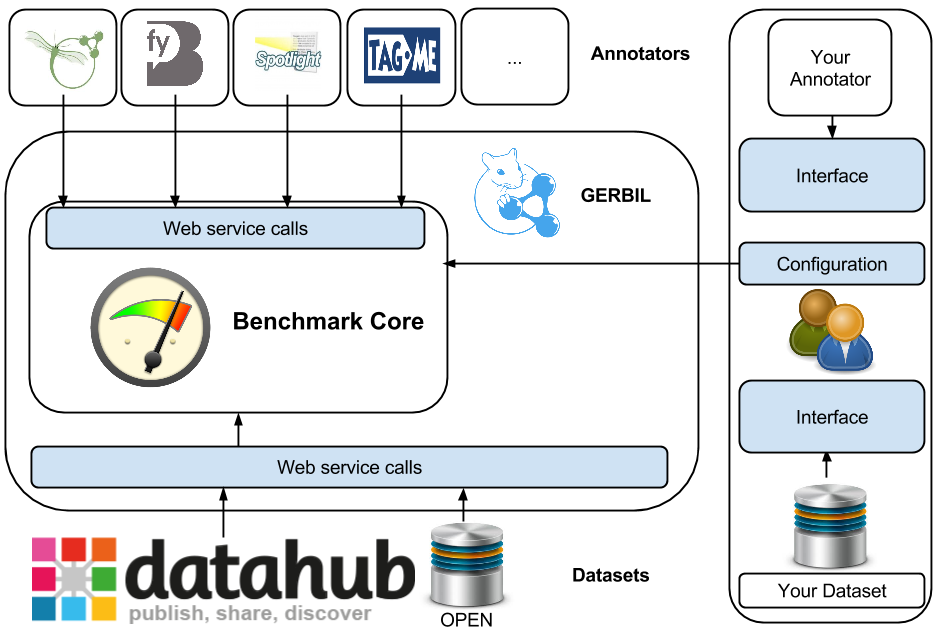
\includegraphics[width=\linewidth]{GERBIL_new_architectur}
\includegraphics[width=0.7\linewidth]{chapter_three/benchmarking/ESWC_GERBIL_demo/gerbiloverview.eps}
%\vspace{-5mm}
\caption{Overview of GERBIL's abstract architecture. Interfaces to users and providers of data sets and annotators are marked in blue.
}
\label{cha333:fig:architecture}
%\vspace{-2mm}
\end{figure}

An overview of GERBIL's architecture is given in Figure~\ref{cha333:fig:architecture}. 
Based on this architecture, we will explain the features that we will present in the demonstration of the GERBIL framework.
%All features will be presented through the online demo at \url{http://gerbil.aksw.org/gerbil}.

\begin{figure}[htb]
\centering
\subfigure[Example spider diagram of recent A2KB experiments with weak annotation matching.]{
\includegraphics[width=0.48\textwidth]{chapter_three/benchmarking/ESWC_GERBIL_demo/results.pdf}
\label{cha333:fig:spiderfmeasure}
}~
\subfigure[Spider diagram of correlations between annotation results and data set features.]{
\includegraphics[width=0.48\textwidth]{chapter_three/benchmarking/ESWC_GERBIL_demo/correlations.pdf}
\label{cha333:fig:spiderfeature}
}
\caption {Spider diagrams generated by the GERBIL interface.}
\end{figure}


\begin{wrapfigure}{l}{6cm}
\centering
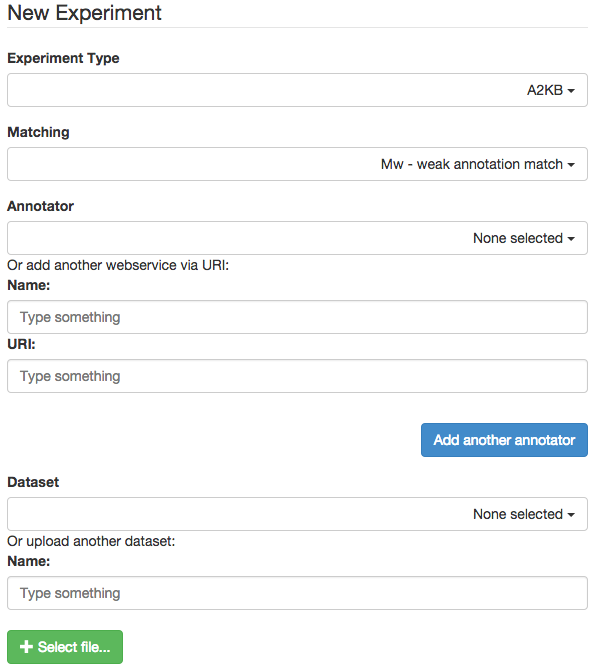
\includegraphics[width=0.95\linewidth]{chapter_three/benchmarking/ESWC_GERBIL_demo/screenshot}
\caption{Experiment configuration screen.}
\label{cha333:fig:screenshot}
\end{wrapfigure}

\textbf{Feature 1: Experiment types.}
An experiment type defines the way used to solve a certain problem when extracting information.
GERBIL extends the six experiments types provided by the BAT framework~\cite{cornolti} (including entity recognition and disambiguation). 
%and extends them by the idea to not only link to Wikipedia but to any knowledge base $K$, see~\cite{GERBIL}.
%The six experiment types implemented in GERBIL are (1) \emph{D2KB}, i.e., disambiguating a set of \emph{given} entity mentions to entities from a given knowledge base or to NIL, (2) \emph{A2KB}, i.e., the classical NER/D task also available as (3) \emph{Sa2KB}, which is the scored annotation task, as well as (4) \emph{C2KB}, i.e., the concept tagging task which aims to detect entities in a given document, also available in a scored variant (\emph{Sc2KB}) and a ranked (\emph{Rc2KB}) version.
With this extension, our framework can deal with gold standard data sets and annotators that link to any knowledge base, e.g., DBpedia, BabelNet~\cite{NavigliPonzetto:12aij} etc., as long as the necessary identifiers are URIs. During the demo, we will show how users can select the type of experiments in the interface (see Figure~\ref{cha333:fig:screenshot}) and explain the different types of experiments.\newline


%\begin{minipage}{0.48\textwidth}
%\end{minipage}
%\hfill
%\begin{minipage}{0.48\textwidth}
%\begin{cha333:table}[htb]
%\centering
%\captionof{cha333:table}{Implemented annotator systems. }
%\label{cha333:tab:annotator}
%\begin{cha333:tabulary}{\columnwidth}{LLC}
%\toprule
%\multicolumn{2}{c}{Annotator}& Experiment\\ 
%\midrule
%\multirow{2}{*}{\cite{milne2008learning}}&Wikipedia                     &\multirow{2}{*}{SA2KB}\\
%&Miner                     &\\
%\cite{rat:rot}&Illionois Wikifier       & SA2KB\\
%\cite{spotlight}&Spotlight            & SA2KB\\
%\cite{TagMe2}&TagMe 2                 & SA2KB\\
%\cite{AIDA}&AIDA                      & SA2KB\\
%\cite{Steinmetz2013}&KEA              & SA2KB\\
%\cite{piccinno2014tagme}&WAT          & SA2KB\\
%\cite{AGDISTIS_ISWC}&AGDISTIS         & D2KB\\
%\cite{babelfy}&Babelfy                & SA2KB\\
%\cite{rizzo2014}&NERD-ML              & SA2KB\\
%\cite{ceccarelli2013dexter}&Dexter   & SA2KB\\
%&NIF-based                     &\multirow{2}{*}{any}\\
%&Annotator                     &\\
%\bottomrule
%\end{cha333:tabulary}
%\end{cha333:table}
%\end{minipage}

%\todo[inline]{AN: Add figure showing the selection of experiment types and matchings. Add reference here and  below (matching section).}

\textbf{Feature 2: Matchings.}
GERBIL offers three types of matching between a gold standard and the results of annotation systems: a \emph{strong entity matching} for URLs, as well as a  \emph{strong} and a \emph{weak annotation matching} for entities.
%(3) \emph{Weak annotation matching $M_w$} has been introduced to relax certain cases. For example,  a gold standard contains a named entity "President Barack Obama" while the result of an annotator only marks "Barack Obama" as named entity. Using an exact matching leads to weighting this result as wrong while a human might rate it as correct. Thus, a correct annotation has to be linked to the same entity and must overlap the annotation of the gold standard.
%(3) \emph{Weak annotation matching $M_w$} relaxes the condition of $M_a$ regarding the position of the entity to allow overlap with the annotation of the gold standard.
The selection and an explanation of the types of matching for given experiments will be part of the demo (see Figure~\ref{cha333:fig:screenshot}). %\todo[inline]{AN: Add ref to figure as requested above.}

\textbf{Feature 3: Metrics.}
Currently, GERBIL offers six measures subdivided into two groups: the micro- and the macro-group of precision, recall and f-measure. As shown in Figure~\ref{cha333:fig:spiderfmeasure}, these results are displayed using interactive spider diagrams that allow the user to easily (1) get an overview of the performance of single tools, (2) compare tools with each other and (3) gather information on the performance on tools on particular data sets. We will show how to interact with our spider diagrams during the demo.

\textbf{Feature 4: Diagnostics.}
An important novel feature of our interface is that it displays the correlation between the features of data sets and the performance of tools (see Figure~\ref{cha333:fig:spiderfeature}). By these means, we ensure that developers can easily gain an overview of the performance of tools w.r.t. a set of features and thus detect possible areas of improvement for future work. 
%End users can make use of these results to select the right tool for their current requirements. Currently, we display correlations with the following data set features: (1) number of documents and (2) number of entities in the data set, (3) entities per document, (4) entities per token, (5) average length of a document as well as (6) the number  of entities of the different types (persons, locations, organizations, etc.). The interface provides these scores by using spider diagrams akin to those used to display the evaluation metrics. We will also show the diagnostics diagrams and explain how to interact with them during the demo. 

\textbf{Feature 5: Annotators.}
The main goal of GERBIL is to simplify the comparison of novel and existing entity annotation systems in a comprehensive and reproducible way.
Therefore, GERBIL offers several  ways to implement novel entity annotation frameworks.
We will show how to integrate annotators into GERBIL by using a Java adapter as well as a \emph{NIF-based Service}~\cite{NIF}.% for communication over web-service in two ways
%: i) if the server-side implementation of annotators understands NIF-documents as input and output format, GERBIL and the framework can simply exchange NIF-documents or ii) if developers do not want to publish their APIs or write source code, GERBIL offers the possibility for NIF-based webservices to be tested online by providing their URI and name only.\footnote{\url{http://gerbil.aksw.org/gerbil/config}} GERBIL does not store these connections in terms of API keys or URLs but still offers the opportunity of persistent experiment results.
Currently, GERBIL offers \overallGERBILannotators entity annotation systems with a variety of features, capabilities and experiments out-of-the-box, including Illinois Wikifier, DBpedia Spotlight, TagMe, AIDA, KEA, WAT, AGDISTIS, Babelfy, NERD-ML and Dexter~\cite{GERBIL}.   
%Table~\ref{cha333:tab:annotator} presents the provided systems and their supported experiment types.
%While AGDISTIS has been in the source code of the BAT-Framework provided by a third-party after publication of Cornolti et al.'s initial work~\cite{Cornolti} in 2014, GERBIL's community effort led to the implementation of overall \numberOfadditionalAnnotators new annotators as well as the before mentioned generic NIF-based annotator.
%The AIDA annotator as well as the "Illinois Wikifier" will not be available in GERBIL since we restrict ourselves to webservices.
%However, these algorithms can be integrated at any time as soon as their webservices are available.
%Upon request, we will show how to integrate annotators into GERBIL by any of these two ways. Especially, we will explain the format of the output that must be generated by a system for GERBIL to be able to interprete it.

\textbf{Feature 6: Data sets.}
Table~\ref{cha333:tab:corpus_stats} shows the \overalldatasets data sets available via GERBIL. 
Thank to the large number of formats, topics and features of the datasets, GERBIL allows carrying out diverse experiments. During the demo, we will show how to add more data sets to GERBIL.

\begin{table*}
    \caption{Features of the data sets and their documents.}
    \begin{tabular}{lp{0.25cm}rp{0.25cm}rp{0.25cm}rp{0.25cm}rp{0.25cm}r}
     \toprule
     Corpus && Topic &&Format &&Experiment && \multicolumn{1}{c}{Size} && \multicolumn{1}{c}{Avg. Entity/Doc.} \\
    \midrule
ACE2004          && news        && MSNBC    && Sa2KB    &&   57 &&   4.44\\
AIDA/CoNLL       && news        && CoNLL    && Sa2KB    && 1393 &&  19.97\\
Aquaint          && news        &&  -       && Sa2KB    &&   50 &&  14.54\\
IITB             && mixed       && XML      && Sa2KB    &&  103 && 109.22\\
KORE 50          && mixed       && NIF/RDF  && Sa2KB    &&   50 &&   2.86\\
Meij             && tweets      && TREC     && Rc2KB    &&  502 &&   1.62\\
Microposts2014   && tweets      &&  -       && Sa2KB    && 3505 &&   0.65\\
MSNBC            && news        && MSNBC    && Sa2KB    &&   20 &&  32.50\\
N$^3$ Reuters-128&& news        && NIF/RDF  && Sa2KB    &&  128 &&   4.85\\
N$^3$ RSS-500    && RSS-feeds   && NIF/RDF  && Sa2KB    &&  500 &&   0.99\\
Spotlight Corpus && news        && NIF/RDF  && Sa2KB    &&   58 &&   5.69\\
%Wiki             && encyclopedic    &&   ? &&   ?\\
	\bottomrule
	\end{tabular}
	\centering
	\label{cha333:tab:corpus_stats}
\end{table*}

%Moreover, we capitalize upon the uptake of publicly available, NIF based corpora over the last years~\cite{yovisto,N3}\footnote{\url{http://datahub.io/data set?license_id=cc-by&q=NIF}}.
%To this end, GERBIL implements a Java-based NIF~\cite{NIF} reader and writer module which enables loading arbitrary NIF document collections, as well as the communication to NIF-based webservices.
%The extensibility of the data sets in GERBIL is furthermore ensured by allowing users to upload or use already available NIF data sets from DataHub. 
%GERBIL will regularly check whether new corpora are available and publish them for benchmarking after a manual quality assurance cycle which ensures their usability for the implemented configuration options.
%Additionally, users can upload their NIF-corpora directly to GERBIL avoiding their publication in publicly available sources.
%This option allows for rapid testing of entity annotation systems with closed source or licenced data sets.

\textbf{Feature 7: Output.}
\label{cha333:sec:output}
GERBIL's main aim is to provide comprehensive, reproducible and publishable experiment results.
Hence, GERBIL's experimental output is represented as a table containing the results, as well as embedded JSON-LD\footnote{\url{http://www.w3.org/TR/json-ld/}} RDF data. During the demo, we will show the output generated by GERBIL for the different experiments implemented and show how the RDF results can be used for the sake of archiving  results. Moreover, we will show how to retrieve experimental results using the permanent URI generated by GERBIL. %We will also show how the results can be queried using SPARQL.

% using the RDF DataCube vocabulary~\cite{datacube}.
%We ensure a detailed description of each component of an experiment as well as machine-readable, interlinkable results following the 5-star Linked Data principles using Linked SDMX~\cite{LinkedSDMX} and DataID~\cite{dataID}.
%Moreover, we provide a persistent and time-stamped URL for each experiment, see Table~\ref{cha333:tab:persistentURL}.

%\begin{cha333:table}
%    \begin{cha333:tabular}{lcr}
%    \toprule
%    Annotator & data set & F1-micro \\
%    \midrule
%    DBpedia Spotlight & IITB & 0.444 \\
%    Babelfy & IITB & 0.377 \\
%    NERD-ML & IITB & 0.488 \\
%    WAT & IITB & 0.202 \\
%    DBpedia Spotlight & KORE50 & 0.265 \\
%    Babelfy & KORE50 & 0.476 \\
%    NERD-ML & KORE50 & 0.238 \\
%    WAT & KORE50 & 0.523 \\
%	\bottomrule
%	\end{cha333:tabular}
%	\centering
%    \caption{Results of an example experiment. It is accessible at \url{http://gerbil.aksw.org/gerbil/experiment?id=201411100001}}
%	\label{cha333:tab:persistentURL}
%\end{cha333:table}

%\emph{RDF DataCube} is a vocabulary standard and can be used to represent fine-grained multidimensional, statistical data which is compatible with the  Linked SDMX~\cite{LinkedSDMX} standard. 
%Every GERBIL experiment is modelled as \texttt{qb:data set} containing the individual runs of the annotators on specific corpora as \texttt{qb:Observations}. 
%Each observation features the \texttt{qb:Dimensions} experiment type, matching type, annotator, corpus and time. 
%The six evaluation measures offered by GERBIL as well as the error count are expressed as \texttt{qb:Measures}. 
%To include further metadata, annotator and corpus dimension properties link \emph{DataID}~\cite{dataID} descriptions of the individual components. 

%GERBIL uses the recently proposed DataID~\cite{dataID} ontology that combines VoID~\cite{void} and DCAT~\cite{dcat} metadata with Prov-O~\cite{prov-o} provenance information and ODRL~\cite{odrl} licenses to describe data sets.
%Besides metadata properties like titles, descriptions and authors, the source files of the open data sets themselves are linked as \texttt{dcat:Distributions}, allowing direct access to the evaluation corpora. 
%Furthermore, ODRL license specifications in RDF are linked via \texttt{dc:license}, potentially facilitating automatically adjusted processing of licensed data by NLP tools. 
%Licenses are further specified via \texttt{dc:rights}, including citations of the relevant publications. 

%To describe annotators in a similar fashion, we extended DataID for services. 
%The class \texttt{Service}, to be described with the same basic properties as data set, was introduced. 
%To link an instance of a \texttt{Service} to its distribution the \texttt{datid:distribution} property was introduced as super property of \texttt{dcat:distribution}, i.e., the specific URI the service can be queried at.
%Furthermore, Services can have a number of \texttt{datid:Parameters} and \texttt{datid:Configurations}.
%data sets can be linked via \texttt{datid:input} or \texttt{datid:output}. 

%Offering such detailed and structured experimental results opens new research avenues in terms of tool and data set diagnostics to increase decision makers' ability to choose the right settings for the right use case.

\section{Evaluation}
\label{cha333:sec:eval}
To ensure that GERBIL can be used in practical settings, we investigated the effort needed to use GERBIL for the evaluation of novel annotators.
To achieve this goal, we surveyed the workload necessary to implement a novel annotator into GERBIL compared to the implementation into previous diverse frameworks. 
Our survey comprised five developers with expert-level programming skills in Java. Each developer was asked to evaluate how much time he/she needed to write the code necessary to evaluate his/her framework on a new data set.
Further details pertaining to this evaluation are reported in the research paper to this demo \cite{GERBIL}.


Overall, the developers reported that they needed between 1 and 4 hours to achieve this goal (4x 1-2h, 1x 3-4h), see Figure~\ref{cha333:fig:comparedTime}.
Importantly, all developers reported that they needed either the same or even less time to integrate their annotator into GERBIL.
This result in itself is of high practical significance as it means that by using GERBIL, developers can evaluate on (currently) \overalldatasets data sets using the same effort they needed for 1, which is a gain of more than 1100\%.
Moreover, all developers reported they felt comfortable---4 points on average on a 5-point Likert scale between very uncomfortable (1) and very comfortable (5)---implementing the annotator in GERBIL.
%Further developers were invited to complete the survey, which is available at our project website.
Even though small, this evaluation suggests that implementing against GERBIL does not lead to any overhead.
Furthermore, the interviewed developers represent a majority of the active research and development community in the are of entity annotation systems.
%On the contrary, GERBIL significantly improves the time-to-evaluation by offering means to benchmark and compare against other annotators respectively data sets within the same effort frame previously required to evaluate on a single data set.

An interesting side-effect of having all these frameworks and data sets in a central framework is that we can now benchmark the different frameworks with respect to their runtimes within exactly the same experimental settings. 
%These results are of practical concern for end users of annotation frameworks as they are most commonly interested in both the runtime and the quality of solutions. 
For example, we evaluated the runtimes of the different approach\-es in GERBIL for the A2KB experiment type on the MSNBC data set, see Figure~\ref{cha333:fig:runtime}.


\begin{figure}[ht]
\centering
\subfigure[Comparison of effort needed to implement an adapter for an annotation system.]{
\includegraphics[width=0.48\textwidth]{chapter_three/benchmarking/ESWC_GERBIL_demo/user_study.eps}
\label{cha333:fig:comparedTime}
%\captionof{cha333:figure}{Example spider diagram of recent A2KB experiments with weak annotation matching derived from our online interface.}
}~
\subfigure[Runtime per document for the A2KB experiment type on the MSNBC data set.]{
\includegraphics[width=0.48\textwidth]{chapter_three/benchmarking/ESWC_GERBIL_demo/needed_times.eps}
\label{cha333:fig:runtime}
%\captionof{cha333:figure}{Spider diagram of results of figure \ref{cha333:fig:spiderfmeasure} and their correlation to data set features.}
}
\caption{Overview of GERBIL evaluation results.}
\end{figure}

\begin{comment}
\section{User Interface}
\label{cha333:sec:usecase}
Compliant with the main goal of GERBIL the reproduction of a certain experiment is central to facilitating research efforts. 
Therefore, our web-based platform offers the opportunity to configure an experiment using the parameters defined in Section~\ref{cha333:sec:architecture}.
The results will be displayed as described above and the experiment itself has a time-stamped URL which is citable and will be stable over time smoothing the way to a new citation quality.
Next to individual configurable experiments, GERBIL offers an overview of recent experiment results and correlations to data set features belonging to the same experiment and matching type in the form of a table as well as sophisticated visualizations\footnote{\url{http://gerbil.aksw.org/gerbil/overview}}, see Figure~\ref{cha333:fig:spiderfmeasure} and Figure~\ref{cha333:fig:spiderfeature}.
This allows for a quick comparison of tools and data sets on recently run experiments without additional computational effort.


\todo[inline]{This is a repetition of section 2.}
\textbf{Adding data sets and annotators.}
GERBIL is designed to be extensible, especially w.r.t. novel data sets and entity annotation systems.
Therefore, we differentiate three ways of integrating such data sets.
(1) A user can upload a NIF-based corpus of documents via our web-interface.
(2) GERBIL downloads data sets from \url{datahub.io} which we will then pull via HTTP requests which will be available after manual revision.
(3) Users can also implement a new data set wrapper source code-wise. 
If users than decide to integrate their wrappers intp GERBILs public repository the community will be further-on able to use it for public evaluations.

Additionally, users can submit new webservice-based entity annotation systems in two different ways:
(1) By providing us with the necessary information to call their NIF-based webservice.
Thereby, they need to enter the webservice's URI and a name for the algorithm.
This methods enables fast prototyping of webservices without the need to implement a BAT-framework annotator wrapper.
To lower barriers, we provide a NIF converter in Java.
(2) Additionally, a user can use our source code project, implement a new annotator and push his source code back to us. 
After a feasibility check, we will then bring the enhanced version of GERBIL online and announce it on the website.
Thus, a tremendous gain with respect to possible comparison opportunities in terms of annotators and data sets is inflicted.

GERBIL also provides an opportunity for closed source data\-set evaluation, e.g., business-relevant data or just experimental data not yet ready to be published.
Users can upload their NIF-based data set via GERBILs web interface.
Apart from the experiment results calculated with it, GERBIL will keep \emph{no} other data of such a data set.
\end{comment}

\section{Conclusion and Future Work}
\label{cha333:sec:conclusion}
In this paper, we presented a demo for GERBIL, a platform for the evaluation of annotation frameworks. We presented the different features that make the GERBIL interface easy to use and informative both for end users and developers. 
With GERBIL, we aim to push annotation system developers to better quality and wider use of their frameworks as well as include the provision of persistent URLs for reproducibility and archiving.
%Furthermore, we implemented a generic adaptor for external data sets as well as a generic interface to integrate remote annotator systems.
%The data sets available for evaluation in the previous benchmarking platforms for annotation was extended by \numberOfadditionaldata sets new data sets. Moreover, \numberOfadditionalAnnotators novel annotators were added to the platform. 
%The evaluation of our framework by contributors suggests that adding an annotator to GERBIL demands 1 to 2 hours of work.
%Hence, while keeping the implementation effort previously required to evaluate on a single data set, we allow developers to evaluate on (currently) \overalldata sets times more data sets.
%The presented, web-based frontend allows for several use cases enabling laymen and expert users to perform informed comparisons of semantic annotation tools and spot flaws w.r.t. the used data set features.
%The persistent URIs enhances the long term quotation in the field of information extraction.
%GERBIL is not just a new framework wrapping existing technology. 
%In comparison to earlier frameworks, it 
GERBIL extends the state-of-the-art benchmarks by the capability of considering the influence of NIL attributes and the ability of dealing with data sets and annotators that link to different knowledge bases. In future work, we aim to provide a new theory for evaluating annotation systems and display this information in the GERBIL interface.
%More information about GERBIL and its source code can be found at the project's website. 

%While developing GERBIL, we spotted several flaws in the formal model underlying previous benchmarking frameworks which we aim to tackle in the future. 
%For example, the formal specification underlying current benchmarking frameworks for annotation does not allow using the scores assigned by the annotators for their results. To address this problem, we aim to develop/implement novel measures into GERBIL that make use of scores (e.g., Mean Reciprocal Rank). 
%Moreover, partial results are not considered within the evaluation. For example, during the disambiguation task, named entities without Wikipedia URIs are not considered. This has a significant impact of the number of true and false positives and thus on the performance of some tools.
%Furthermore, certain tasks seem to be too coarse. For example, we will consider splitting the Sa2KB and the A2KB tasks into two subtasks: The first subtask would measure how well tools perform at finding named entities inside the text (NER task) while the second would evaluate how well tools disambiguate those named entities which have been found correctly (similar to the D2KB task).
%Moreover, we plan to provide information about the point in time since when an annotator is stable, i.e., the algorithm underlying the webservice has not changed so as to provide end users with metadata on when to use which annotator.


%\bibliographystyle{abbrv}
%\bibliography{myrefs}


%\end{document}


\chapter{Developing a Sustainable Platform for Entity Annotation Benchmarks}

%\author{
%Michael Röder \and
%Ricardo Usbeck \and 
%Axel-Cyrille Ngonga Ngomo
%}

%\institute{
%University of Leipzig, Germany\\\email{\{roeder,usbeck,ngonga\}@informatik.uni-leipzig.de}
%}

%\maketitle
%\todo[inline]{Focus on lessons learnt, mention how people can use your software. Accepted development papers will be published in the CEUR-WS workshop proceedings series.}

%\begin{abstract}
The existing entity annotation systems that drive the extraction of RDF from unstructured data are hard to compare as their evaluation relies on different data sets and measures. 
%growing amount of unstructured data on the Document Web and the rising number of tools for structured data from the Web of Data created the need for a growing
%number of entity annotation systems is hard to compare, making it difficult for developers to decide their published experiments are nearly unrepeatable and the diversity of data sets is tremendous.
We developed GERBIL, an evaluation framework for semantic entity annotation that provides developers, end users and researchers with easy-to-use interfaces for the agile, fine-grained and uniform evaluation of 9 annotation tools on 11 different data sets within 6 different experimental settings on 6 different measures. 
In this paper, we present the developed interfaces, data flows and data structures. Moreover, we show how GERBIL supports a better reproducibility and archiving of experimental results.
%Finally, we will explain how to use GERBIL from various perspectives and discuss why this community effort will support semantic annotation research in the long term.
%\end{abstract}


\section{Introduction}
The need for extracting structured data from text has led to the development of a large number of tools dedicated to the extraction of structured data from unstructured data (see~\cite{GERBIL} for an overview).
%The issue of  comparability of results is not to be regarded as being intrinsic to the annotation task.
While these tools do provide evaluation results, these results are rarely fully comparable as they commonly rely on different data sets or different measures. This is partly due to data preparation being a tedious problem in the annotation domain due to the different formats of the gold standards as well as the different data representations across reference data sets.
%These restrictions have led to authors evaluating their approaches on data sets (1) that are available to them and (2) for which writing a parser as well as of (3) an evaluation tool can be carried out with reasonable effort.
%Furthermore, diverse (4) quality measures have been developed and used actively across the annotation research community to evaluate the same task, leading to different results across publications which are not easily comparable. 
Recently, benchmarking frameworks such as the BAT-framework~\cite{cornolti} or NERD-ML~\cite{rizzo2014} for entity annotation systems have began addressing the problem on reproducible experiments for entity annotation.
With GERBIL\footnote{More information and a demo can be found at \url{http://gerbil.aksw.org}} 
 we aim to unify experiment setups, ease implementation and testing effort as well as contribute to an open, repeatable, publishable and archivable open science area to foster an active community of entity annotation tool developers. 

GERBIL goes beyond the state of the art by extending the BAT-framework~\cite{cornolti} as well as Nerd-ML~\cite{rizzo2014} in several dimensions. In particular we provide fine-grained diagnostics for annotation tools, enhanced reproducibility through archiving experiments and assigning URIs to them, easily publishable results by providing results both as RDF (for machines) and tables (for humans).
Overall, we provide the following features:

\textbf{Feature 1: Extensible experiment types.}
An experiment type defines the way used to solve a certain problem when extracting information.
GERBIL extends the six experiment types provided by the BAT framework~\cite{cornolti} (including entity recognition and disambiguation) towards more general, URI based experiments.
%Additionally, we are working on the implementation of an entity typing experiment as it is defined in the Open Knowledge Extraction Challenge 2015\footnote{\url{http://2015.eswc-conferences.org/important-dates/call-OKEC}}.
% as well as it implements 3 experiment types for the Open Knowledge Extraction Challenge 2015\footnote{\url{http://2015.eswc-conferences.org/important-dates/call-OKEC}}.
%\todo[inline]{Micha: Ich finde das nicht so gut, dass wir immer Dinge ins Paper schreiben, die wir noch gar nicht gemacht haben. Wir können gern reinschreiben, dass wir das "Entity Typing" als weiteren Experimenttyp einbringen. Aber mehr haben wir im Moment ja noch gar nicht.}
With this extension, our framework can deal with gold standard data sets and annotators that link to any knowledge base as long as the necessary identifiers are URIs.

\textbf{Feature 2: Matchings.}
GERBIL offers three types of matching between a gold standard and the results of annotation systems: a \emph{strong entity matching} for URIs, as well as a  \emph{strong} and a \emph{weak annotation matching} for entities.

\textbf{Feature 3: Measures.}
Currently, GERBIL offers six measures subdivided into two groups: the micro- and the macro-group of precision, recall and f-measure. As shown in Figure~\ref{cha334:fig:spiderfmeasure}, these results are displayed using interactive spider diagrams that allow the user to easily (1) get an overview of the performance of single tools and (2) compare tools.% with each other.
%and (3) gather diagnostic insights on the performance of tools on particular data sets.

Explicit definitions can be found in Usbeck et al.~\cite{GERBIL}.

\textbf{Feature 4: Diagnostics.}
An important novel feature of our interface is that it displays the correlation between the features of data sets and the performance of tools (see Figure~\ref{cha334:fig:spiderfeature}). By these means, we ensure that developers can easily gain an fine-grained overview of the performance of tools
%w.r.t. a set of features 
and thus detect possible areas of improvement for future work. 



\begin{figure}[htb]
\centering
\subfigure[Example spider diagram of recent A2KB experiments with weak annotation matching.]{
\includegraphics[width=0.48\textwidth]{chapter_three/benchmarking/ESWC_2015_DEV_GERBIL/results.pdf}
\label{cha334:fig:spiderfmeasure}
}~
\subfigure[Spider diagram of correlations between annotation results and data set features.]{
\includegraphics[width=0.48\textwidth]{chapter_three/benchmarking/ESWC_2015_DEV_GERBIL/correlations.pdf}
\label{cha334:fig:spiderfeature}
}
\caption {Spider diagrams generated by the GERBIL interface.}
\end{figure}


\textbf{Feature 5: Annotators.}
Currently, GERBIL offers \overallGERBILannotators entity annotation systems with a variety of features, capabilities and experiments out-of-the-box. 

\textbf{Feature 6: Data sets.}
The latest version of GERBIL offers \overalldatasets data sets.
Thanks to the large number of formats, topics and features of the data sets, GERBIL allows carrying out diverse experiments.

\textbf{Feature 7: Output.}
\label{cha334:sec:output}
GERBIL's experimental output is represented as a table containing the results, as well as embedded JSON-LD\footnote{\url{http://www.w3.org/TR/json-ld/}} RDF data for the sake of archiving experiment results and additional information, e.g., the version of GERBIL that has been used.
Moreover, GERBIL generates a permanent URI for each experimental result.

%To ensure that our framework is useful to both end users and tool developers, its architecture and interface were designed to allow (1) the easy integration of annotators through REST services, (2) the easy integration of data sets via DataHub\footnote{\url{http://datahub.io}} and file uploads, (3) the addition of new performance measures, (4) the provision of diagnostics for tool developers and (5) the portability of results. 

In this paper, we will give a detailed explanation of the different RDF data structures underlying GERBIL's architecture.
We will explain the internal workflow of GERBIL and argue why it simplifies the implementation of further experiments, annotators, data sets, matchings and measures.
%Additionally, we will explain our plans for the longevity of GERBIL as platform for entity annotation systems and 
We conclude by pointing at future work.

%In this paper, we will give a detailed explanation on how the different interfaces are implemented and reason why GERBIL eases the implementation of further annotators, data sets, matchings and measures. % based on the example of the OKE-Challenge.
%We will explain GERBIL's inner dataflow and its importance towards an efficient and scalable experimental platform.
%Furthermore, we will give an in-depth introduction to the underlying RDF data used to described whole experiments and the explain our plans for the longevity of GERBIL as platform for entity annotation systems. 
%Finally, we discuss the impact of design decisions and point towards future work. 


\section{GERBIL's interfaces, dataflow, structure}
\label{cha334:sec:architecture}

\begin{comment}
\subsection{Uses Cases}
Currently, the architecture allows at least three basic use cases: 

\textbf{Repeat already published experiments.}
Compliant with the main goal of GERBIL the reproduction of a certain experiment is central to facilitating research efforts.
Thus, GERBIL offers the opportunity to configure an experiment using four parameters: Experiment type, matching, annotator and data set.
The results will be displayed as table and embedded JSON-LD RDF via a time-stamped URI which can be cited and is stable over time.

\textbf{Run evaluations based on novel data sets.}
GERBIL differentiates three ways of integrating such data sets.
(1) A user can upload a NIF-based corpus (see Section~\ref{cha334:sec:datastructures}) via our web-interface. 
This allows the usage of \emph{closed source} data sets, e.g., business-relevant data or just experimental data not yet ready to be published.
Apart from the experiment results calculated with it, GERBIL will keep \emph{no} other data of such a data set.
(2) GERBIL is able to download NIF-based data sets from \url{datahub.io}.% which will be available after manual revision or
(3) Users can also implement a new data set wrapper source code-wise. 
%While options (1,2) demand knowledge of the NIF format, option (3) uses Java-based wrapper methods to make even legacy data available.
%Furthermore, option (1) allows for the evaluation of \emph{closed source} data set evaluation, e.g., business-relevant data or just experimental data not yet ready to be published.
%Apart from the experiment results calculated with it, GERBIL will keep \emph{no} other data of such a data set.

\textbf{Evaluating a new algorithm.}
Finally, users can submit new webservice-based entity annotation systems in two different ways:
(1) By providing GERBIL with the NIF-based webservice's URI.
This method enables fast prototyping of webservices without the need to implement an annotator wrapper.
To lower barriers, we provide a NIF converter in Java \footnote{\url{https://github.com/AKSW/gerbil/tree/gerbil.nif.transfer}}.
(2) Additionally, a user can use our source code project, implement a new annotator and push his source code back to us. 
%After a feasibility check, we will then bring the enhanced version of GERBIL online and announce via various channels.
%Thus, a tremendous gain with respect to possible comparison opportunities in terms of annotators and data sets is inflicted.
\end{comment}

\subsection{Datastructures}
\label{cha334:sec:datastructures}

GERBIL unifies the different formats used by existing datasets and annotators.
To this end, GERBIL's interfaces are mainly based on the \emph{NLP Interchange Format} (NIF).
This is a RDF-based Linked Data serialization which provides several advantages such as interoperability by standardization or query-ability.
The \emph{NIF-standard} assigns each document an URI as starting point and generates another Linked Data resource per semantic entity.
Each document is a resource of type \texttt{nif:Context} and its content is the literal of its \texttt{nif:isString} predicate. 
Every entity is an own resource with a newly generated URI pointing to the original document via the \texttt{nif:referenceContext} predicate.
Additionally the begin (\url{nif:beginIndex}) and end position (\url{nif:endIndex}) as well as the disambiguated URI (\url{itsrdf:taIdentRef}) and the respective KB (\url{itsrdf:taSource}) are stored.
NIF's paramount position amongst corpora serialisation formats is evident by the growing number of available datasets~\cite{GERBIL}.\footnote{The prefix \texttt{nif} stands for \url{http://persistence.uni-leipzig.org/nlp2rdf/ontologies/nif-core\#} while \texttt{itsrdf} is short for \url{http://www.w3.org/2005/11/its/rdf\#}.}

GERBIL's main aim is to provide comprehensive, reproducible and publishable experiment results.
Thus, GERBIL enforces the use of a machine-readable description for each experiment via JSON-LD\footnote{\url{http://www.w3.org/TR/json-ld/}} RDF data using the RDF DataCube vocabulary~\cite{datacube} next to a human-readable table presentation.
The \emph{RDF DataCube} vocabulary can be used to represent fine-grained multidimensional, statistical data which is compatible with the Linked SDMX~\cite{LinkedSDMX} standard. 
GERBIL models each experiment as \texttt{qb:Dataset} containing \texttt{qb:Observations} for each individual run of a annotator on a dataset.
Each observation features the \url{qb:Dimensions} experiment type, matching type, annotator, corpus, and time. 
The evaluation measures and an error count are expressed as \texttt{qb:Measures}.\footnote{\texttt{qb} is a prefix for for \url{http://purl.org/linked-data/cube\#}.} 

GERBIL relies on the DataID ontology~\cite{dataID} to represent further metadata as well as annotator and corpus information. 
Besides metadata properties like titles, descriptions and authors, the source files of the open datasets themselves are linked as \url{dcat:Distributions}, allowing direct access to the evaluation corpora. 
Furthermore, ODRL license specifications in RDF are linked via \texttt{dc:license}, potentially facilitating automatically adjusted processing of licensed data by NLP tools. 
Licenses are further specified via \texttt{dc:rights}, including citations of the relevant publications.\footnote{The prefix \texttt{dcat} stands for \url{http://www.w3.org/ns/dcat\#} while \texttt{dc} is short for \url{http://purl.org/dc/elements/1.1/}.}
To describe annotators in a similar fashion, we extended DataID for services. 
The class \texttt{Service}, to be described with the same basic properties as dataset, was introduced. 
To link an instance of a \texttt{Service} to its distribution the \texttt{datid:distribution} property was introduced as super property of \texttt{dcat:distribution}, i.e., the specific URI the service can be queried at.
Furthermore, Services can have a number of \texttt{datid:Parameters} and \texttt{datid:Configurations}.
Datasets can be linked via \texttt{datid:input} or \texttt{datid:output}.\footnote{\texttt{datid} is a prefix for for \url{http://dataid.dbpedia.org/ns/core\#}.} 
%Using this detailed description of an experiment opens new research avenues, e.g., tool diagnostics and decision maker support, at the same time as providing provenance information.
%Especially, using RDF as experiment description allows for the extension and adaption of the experimental metadata format on-the-fly.
An example JSON-LD for an archived experiment can be found below.


\scriptsize
%	  \begin{lstlisting}[language=JSON]
\begin{minted}{json}

{
  "@graph" : [ {
    "@id" : "http://gerbil.aksw.org/gerbil/experiment?id=...#experiment_...",
    "@type" : [ "gerbil:Experiment", "qb:Dataset" ],
    "experimentType" : "gerbil:A2KB",
    "matching" : "gerbil:WeakAnnoMatch",
    "structure" : "gerbil:dsd",
    "label" : "Experiment 201503160001"
  }, {
    "@id" : "http://gerbil.aksw.org/gerbil/experiment?id=...#experiment_..._task_0",
    "@type" : "qb:Observation",
    "annotator" : "http://gerbil.aksw.org/gerbil/dataId/corpora/Babelfy",
    "dataset" : "http://gerbil.aksw.org/gerbil/dataId/annotators/ACE2004",
    "statusCode" : "-1",
    "timestamp" : "2015-03-16T12:31:52.469Z"
  } ],
  "@context" : {
    ...
  }
}
\end{minted}
\normalsize

\subsection{Workflow}
\begin{figure}[tb]
    \centering
    \includegraphics[width=0.9\linewidth]{chapter_three/benchmarking/ESWC_2015_DEV_GERBIL/gerbiloverview.eps}
    \caption{Overview of GERBIL's abstract architecture. Interfaces to users and providers of data sets and annotators are marked in blue.}
    \label{cha334:fig:architecture}
\end{figure}
Figure \ref{cha334:fig:architecture} shows the architecture of GERBIL with the data sets at the bottom, the annotators in the top and the user interface as well as user defined annotator and data set at the right.
A GERBIL session starts at the configuration screen with which a user defines the experiment he is interested in.
Each experiment is divided into tasks.
A task comprises the evaluation of a single annotator using a single data set, is encapsulated into fault-tolerant classes and runs inside an own thread.
Our fault-tolerance classes at two types of errors: (1) an annotator may return error codes for single documents, e.g., because of the missing ability to handle special characters.
While other evaluation frameworks tend to cancel the experiments after an exception thrown by the annotator, GERBIL counts these smaller errors and reports them as part of the evaluation result.
The second type of fault tolerance aims at (2) larger errors, e.g., the data set couldn't be loaded or the annotator is unreachable via its Web service.
These run-time errors are handled by storing one of the predefined error codes inside the experiment database.
Therewith, we ensure that the user gets instant feedback if some parts of the experiment couldn't be performed as expected.

During a task, the single documents of a data set are sent to the annotator.
After finishing the last document, the responses are evaluated.
Currently, the evaluation is focused on the quality, i.e., precision, recall, F1-score and error counts, but can be extended.
Moreover, a runtime is also available~\cite{GERBIL}.
For some experiment types, e.g., the entity-linking tasks, the evaluation needs additional information.
GERBIL is able to search for \texttt{owl:sameAs} links to close the gap between data sets and annotators that are based on different knowledge bases.
Currently, this search is mainly based on the information inside the data set and retrieval of the entity mentioned by the annotator.
The search could be extended by using local search indexes that contain mappings between well-known knowledge bases, e.g., DBpedia and Freebase.
The results are currently written to an HSQL database\footnote{\url{http://hsqldb.org/}}.

\subsection{Extensible Interfaces}

The workflow of GERBIL is very general.
An experiment has a certain experiment type, a matching, and a couple of datasets and annotators.
Thus, it is easily possible to add new experiment types to GERBIL that are not part of the system, e.g., word sense disambiguation.
One major advantage towards this form of extensibility is the usage of NIF for transferring the single documents.
Since NIF is based on RDF the documents sent and received by the system as well as the datasets can be enriched with further information that can be used for the experiments.
Thus, it is easy to add a new experiment type even if the type needs information that cannot be expressed with NIF, e.g., the entity typing task defined in the Open Knowledge Extraction Challenge 2015\footnote{\url{http://2015.eswc-conferences.org/important-dates/call-OKEC}}.
For this challenge, an adapted version of GERBIL has been developed\footnote{\url{https://github.com/AKSW/gerbil/releases/tag/OKE2015}}.
In this version, an annotator that is able to identify the type of a new, unknown entity adds this type to the RDF model of its response.
This information can't be understood directly by the response handling, but is kept and made available to the evaluation component of GERBIL.
Thus, this type information can be used to evaluate the typing performance of an annotator.

%\subsection{Long-term stability}

%Moreover, the research and development unit of the University Leipzig Computation Center will keep daily backups to ensure long-term quotability.

\section{Conclusion and Future Work}
\label{cha334:sec:conclusion}
In this paper, we presented GERBIL, a platform for the evaluation, publishing and archiving of semantic entity annotation experiments.
GERBIL extends the state-of-the-art benchmarks by dealing with data sets and annotators that link to different knowledge bases. 
Furthermore it offers extensible interfaces, reliable experiment descriptions as well as diagnostics and decision support.
Our future work will comprise a better experiment task scheduling to achieve a higher efficiency. 
%GEBRIL has a high potential to save memory if the experiment tasks could share their common elements, e.g., the data sets they are working on.
Another task is the improvement of the user interface towards a better intelligibility.
Finally, we will devise a solution to ensure that GERBIL remains available to the community for the years to come.

%As GERBIL is still a young project and thus we are trying to explore the borders of our endeavour. 
%As GERBIL has been launched within several PhD projects funded by European Social Fund and several other European and German research grants the deployment of GERBIL is safeguarded within the next five years.
%Furthermore, we have two fallback solutions: (1) the research group AKSW and the university computing center which currently already hosts more than 30 open source projects announced a strong partnership with the GERBIL platform.
%(2) GERBIL is open source software which can be maintained and hosted by anybody.

%\bibliographystyle{abbrv}
%\bibliography{myrefs}


%\end{document}


\part{Question Answering on hybrid sources}
\cleardoublepage
\ctparttext{
    The third part 
}


% ********************************************************************
% Backmatter
%*******************************************************
\appendix
\cleardoublepage
\part{Appendix}
%\include{Chapters/12/12_appendix}
%********************************************************************
% Other Stuff in the Back
%*******************************************************
\cleardoublepage%********************************************************************
% Bibliography
%*******************************************************
% work-around to have small caps also here in the headline
\manualmark
\markboth{\spacedlowsmallcaps{\bibname}}{\spacedlowsmallcaps{\bibname}} % work-around to have small caps also
%\phantomsection 
\refstepcounter{dummy}
\addtocontents{toc}{\protect\vspace{\beforebibskip}} % to have the bib a bit from the rest in the toc
\addcontentsline{toc}{chapter}{\tocEntry{\bibname}}
\bibliographystyle{apalike}
\label{app:bibliography} 
\bibliography{Bibliography}

%\todo[inline]{fix bibiography entries in bib file}
%\cleardoublepage\pagestyle{empty}

\hfill

\vfill


\pdfbookmark[0]{Colophon}{colophon}
\section*{Colophon}
This document was typeset using the typographical look-and-feel \texttt{classicthesis} developed by Andr\'e Miede. 
The style was inspired by Robert Bringhurst's seminal book on typography ``\emph{The Elements of Typographic Style}''. 
\texttt{classicthesis} is available for both \LaTeX\ and \mLyX: 
\begin{center}
\url{http://code.google.com/p/classicthesis/}
\end{center}
Happy users of \texttt{classicthesis} usually send a real postcard to the author, a collection of postcards received so far is featured here: 
\begin{center}
\url{http://postcards.miede.de/}
\end{center}
 
\bigskip

\noindent\finalVersionString

%Hermann Zapf's \emph{Palatino} and \emph{Euler} type faces (Type~1 PostScript fonts \emph{URW
%Palladio L} and \emph{FPL}) are used. The ``typewriter'' text is typeset in \emph{Bera Mono}, 
%originally developed by Bitstream, Inc. as ``Bitstream Vera''. (Type~1 PostScript fonts were made 
%available by Malte Rosenau and
%Ulrich Dirr.)

%\paragraph{note:} The custom size of the textblock was calculated
%using the directions given by Mr. Bringhurst (pages 26--29 and
%175/176). 10~pt Palatino needs  133.21~pt for the string
%``abcdefghijklmnopqrstuvwxyz''. This yields a good line length between
%24--26~pc (288--312~pt). Using a ``\emph{double square textblock}''
%with a 1:2 ratio this results in a textblock of 312:624~pt (which
%includes the headline in this design). A good alternative would be the
%``\emph{golden section textblock}'' with a ratio of 1:1.62, here
%312:505.44~pt. For comparison, \texttt{DIV9} of the \texttt{typearea}
%package results in a line length of 389~pt (32.4~pc), which is by far
%too long. However, this information will only be of interest for
%hardcore pseudo-typographers like me.%
%
%To make your own calculations, use the following commands and look up
%the corresponding lengths in the book:
%\begin{verbatim}
%    \settowidth{\abcd}{abcdefghijklmnopqrstuvwxyz}
%    \the\abcd\ % prints the value of the length
%\end{verbatim}
%Please see the file \texttt{classicthesis.sty} for some precalculated 
%values for Palatino and Minion.
%
%    \settowidth{\abcd}{abcdefghijklmnopqrstuvwxyz}
%    \the\abcd\ % prints the value of the length





\cleardoublepage%*******************************************************
% Declaration
%*******************************************************
\refstepcounter{dummy}
\pdfbookmark[0]{Declaration}{declaration}
\chapter*{Declaration}
\thispagestyle{empty}
This thesis is a presentation of my original research work. Wherever contributions of others are involved, every effort is made to indicate this clearly, with due reference to the literature, and acknowledgement of collaborative research and discussions.
\bigskip
 
\noindent\textit{\myLocation, August 2015}

\smallskip

\begin{flushright}
    \begin{tabular}{m{5cm}}
        \\ \hline
        \centering\myName \\
    \end{tabular}
\end{flushright}

% ********************************************************************
% Game Over: Restore, Restart, or Quit?
%*******************************************************
\end{document}
% ********************************************************************
